\documentclass[twoside,a4paper]{report}
\usepackage{amssymb,amsmath}
\usepackage[mathletters]{ucs}
\usepackage[utf8x]{inputenc}
\usepackage[breaklinks=true,unicode=true,pdfborder={0 0 0},colorlinks=false]{hyperref}
\usepackage{listings}
\lstdefinelanguage{obftool}{morekeywords={help,quit,status,parse,explore,format,visualise,reorder,mark}}
\lstset{language=Python, numbers=left, showstringspaces=false, frame=single}
\usepackage{pst-gantt}
\setlength{\parindent}{0pt}
\setlength{\parskip}{6pt plus 2pt minus 1pt}
\setcounter{secnumdepth}{0}
\usepackage[dvips]{graphicx}
\usepackage{subfig}

% For title page
\newcommand{\HRule}{\rule{\linewidth}{0.5mm}}

\begin{document}
\begin{titlepage}

\begin{center}

% Upper part of the page
\textsc{\LARGE Imperial College London}\\[1.5cm]
\textsc{\Large Undergraduate Individual Project}\\[0.5cm]

% Title
\HRule \\[0.4cm]
{\huge \bfseries Obfuscating Python 3000} \\[0.4cm]
\HRule \\[0.4cm]

Code on git at: ssh://user@shell4.doc.ic.ac.uk/homes/asg08/git/ugproject.git \\[1.5cm]

% Author and supervisor
\begin{minipage}{0.4\textwidth}
\begin{flushleft} \large
\emph{Author:}\\
Andy Gurden
\end{flushleft}
\end{minipage}
\begin{minipage}{0.4\textwidth}
\begin{flushright} \large
\emph{Supervisor:} \\
Herbert Wiklicky
\end{flushright}
\end{minipage}

\vfill

% Bottom of the page
{\large \today}

\end{center}
\end{titlepage}

\cleardoublepage

\begin{abstract}
\#TODO write abstract!
\end{abstract}

\section*{Acknowledgements}

TODO - write acknowledgements - Hayley Hannam, Herbert Wiklicky, Chris Hankin, Alex Lamaison

\tableofcontents

\clearpage

\section{Introduction}

With the increasing popularity of interpreted languages like Java or Python, we are starting
to see a change in the way that program code is distributed.

Not so long ago, a programmer could write their program in a compiled language such as C. This would then be compiled
to machine code for a given architecture, and the program could be handed out to anyone without
worrying about whether a hacker or reverse-engineer could recover the original source code.
Of course, it can be done and there are tools to reverse the translation, called decompilers \cite{cdecomp}, but it
is a difficult process and there are methods to make this harder \cite{disres}.

The difference for interpreted languages is that much more of the original code is kept in the
distributed format. Java code, for example, is usually distributed as bytecode for the Java Virtual
Machine (JVM). This still holds information about high level constructs such as class and method names \cite{classinfo},
making it much easier to decompile a Java class.

In a language like Python it is usually raw source code that is distributed, therefore a
user need not put in any effort to view the inner workings of the program. While this is good
for the security of a user \cite{noobf}, it is often the case that the author will not want sensitive,
perhaps proprietary, parts of their code open to inspection or theft. With this in mind, we will work on ways to protect it.

We should note that there are existing solutions for the protection of Python source code, examples of which vary in quality.
These will be discussed in the next section, along with their drawbacks and areas to which we can contribute further.

The approach we will take to the above problem is to obfuscate the Python source code. This technique involves changing the
original program in some way so that it is more confusing to a reader or more difficult to analyse, while still remaining correct.

More specifically, during this project we shall implement a basic functioning, but extensible, obfuscator
that can modify the control flow of a program with the aim of diverting a human reader from its actual
function. This will act upon Python source code and should help to address the issues described when distributing source code.
In the interest of evaluation, we will also create a sister program that will try to reverse the modifications performed by the
obfuscator with the aim of recovering the original source code. 
We shall aim to create these tools by taking a subset of obfuscation techniques used on other languages (e.g.
loop flattening or instruction reordering \cite{taxobftrans}) and looking at how well these will transfer to such a dynamic language as Python.

On the surface this may appear rather simple, however as Python is such a highly dynamic language it can be very difficult to analyse
\cite[p13]{staticanal} as thoroughly as a more traditional compiled language such as Java. In such traditional languages, it is much easier to perform a static
analysis of the code. This is simply not feasible for many applications in Python, yet many program transformations will require this type of
thorough analysis. Issues in this area may appear or they may not, depending on the techniques we decide to implement, and it will be a part of
this project to notice and evaluate these issues.

\section{Background}

Here we will discuss Python and some solutions for protecting code, as well as some obfuscation techniques
and current tools.

\subsection{Python}

As we have described in the introduction, the project aims to implement known obfuscation techniques specifically on Python source code.
The language is used widely, from the popular web framework Django \cite{django} through many applications
from Google \cite{pygoogle} and even embedded as a scripting language for extensions in programs like GNU
Image Manipulation Program (GIMP) \cite{gimp}. Due to its wide and varied use, it is of increased importance
that someone wishing to protect their Python code from theft or reverse-engineering can do so.

To be specific about the code and techniques, we will restrict our efforts to using obfuscation methods that will
result in standard Python code so that it is portable across any of the many Python runtime implementations. The version
of Python we will be working with is 3.x (nicknamed 3000 or py3k) for both source and generated code. The most popular
version of Python is still 2.x, however this version will soon ``become stale'' as the language moves towards 3.x, on its way
dropping some compatibility with 2.x.

\subsubsection{Methods of Protection}

There are a number of ways Python developers currently try to hide or protect their code, with varying degrees
of success and security.

One method is to use a Python tool called Freeze. This tool will simply take given source code and compile
it to bytecode. A Unix executable will then be created containing the necessary parts of the Python runtime as
well as the bytecode to allow a program to run
on systems without Python installed. As it says in the README \cite{freezereadme} this provides little if any
protection as Python's standard library comes with a disassembler ready to view the bytecode. There are also
tools such as AntiFreeze \cite{pirates} to help analyse the code, and a program called
decompyle \cite{decompyle} that will actually try to generate the original source for older bytecode ($\le$version
2.3). There is a similar tool to Freeze, called py2exe \cite{py2exe}, that will create a Windows executable but
this too suffers from the same problems.

From the above paragraph, it is easy to spot that just distributing the Python bytecode, another method occasionally
used, also fails to thwart reverse-engineering attempts. In fact there is another problem
with these methods and any others that rely on Python bytecode. Bytecode is an implementation detail \cite{dis}
of the default Python implementation, CPython. Relying on this to distribute code would glue any
user to a specific implementation of Python and possibly even to a specific version. This would remove the portability
expected from a Python program and contradict our own condition that solutions must be portable, specified earlier.

A more secure solution for protecting Python code, and one that works for many people, is to remove the most
sensitive parts and replace them with C extensions to the Python program. This way the code becomes machine
code; it can use the wealth of obfuscation tools for C and being compiled machine code makes it much
harder to reverse engineer. Again though, this is based on CPython's ability to include C modules, restricting a
user to a particular runtime as well as a particular machine architecture (that the modules are compiled for).

A portable way to protect the code would be to obfuscate it, performing source to source translations that can
confuse a reader or program analyser. This is not and will never be a perfect solution, because all attempts
to avoid reverse engineering will be overcome eventually. The difference between one method of protection and
another is the time and effort taken to break each and how much the result is worth to the attacker. There are already
programs for obfuscating Python code, though the selection is limited. These will be discussed later.

\subsubsection{Ethics of Obfuscating}

Although it may not be obvious, there are ethical and possibly even legal implications to obfuscation.
Specifically for Python, the language is based on a philosophy of clear and readable code, and actually
enforces this by the design of the grammar. Obviously, obfuscation is an attempt to take this away.

This hits out against certain expectations a user may have about a Python program. A key benefit of having your
software handed to you in source form is that you always know what it is doing. Deliberately obscuring the
function of software, but in a format that is almost always open for inspection, removes trust. The vendor or developer is
denying the user their trust by not allowing them to use the software as they wish, but more importantly the user's
trust in the software can be lost.

If the software is hiding what it is doing this could be for a legitimate reason, such as hiding novel ideas
from competitors, or it could be to mask malicious content. A user or program, provided the obfuscation is
good enough, cannot tell which the reason is. This is a technique often employed by malware
writers to avoid detection by anti-virus software \cite{dycodeobf}. In fact, it has been argued that any and
all obfuscated code should be treated as if it were malware \cite{noobf}, assuming software is guilty until
proven otherwise.

Our view and the view we will take for the remainder of the paper is that these issues create more reason for
building a tool such as this. By allowing issues such as those described above to block research into a subject
we are making ourselves much more vulnerable to those who would abuse the technology. Therefore those who choose to abuse any
product of this project will be free to do so, just as will those who would use the tools and information legitimately.

It is important to note that although our conclusion on this subject would be the same were we based outside of
the UK, the legal implications stemming from it may not be. For example in German law, clause 202(c) \cite{202c}
could make it illegal to write or distribute this software if it could be used for
certain forms of cybercrime. As discussed above, it probably could, and would have implications for anyone distributing
or using the information presented here.

In the UK we have a similar law in the Computer Misuse Act section 3A \cite{compmisuse}. This laws says that a person is guilty of an offence
if they supply a software tool intended for or likely to be used in a criminal manner. The breaking of this law carries a fine or a maximum 12 month
prison sentence, but we believe it unlikely that any software we create will be used for criminal purposes. There are
much better methods to hide malware from an unsuspecting user.

\subsection{Types of Obfuscation}

Having decided to obfuscate the code from source to source, it is worth taking a look at the types of
obfuscation already used, how they are useful and which we will pursue. We will classify these types into 3 categories
as suggested by \cite[p10]{desevobf}.

\subsubsection{Layout Obfuscation}

These will apply transformations to the source source or possibly bytecode that do not affect the running of the
program. This is a very common form of obfuscation \cite[p10]{desevobf}, and involves transformations such as removing comments,
scrambling identifiers, or removing as much whitespace as possible to make the code unreadable.

Comments and identifiers often hold a lot of semantic information as they are designed to do.
Removal of this information by deletion or renaming is quite effective and almost always irreversible. Other transformations involving
structure and whitespace
can be easily removed by a source formatter and so will only be effective against an impatient human.

While some of these transformations may be easy to perform in traditional languages, there are places in which
Python's design can cause problems. Fortunately these kinds of transformations are already available using existing
tools, although these are not necessarily compatible with Python 3. For these reasons, we will be focusing on other forms of
obfuscation which have received less attention.

\subsubsection{Data Obfuscation}

This type of obfuscation transforms data layout and can help to obfuscate the structure of the program. It can be
particularly helpful in Python as the language makes it very easy to inspect programs as they run, enabling dissection of internal data
structures to learn about how the program works.

We can look towards Collberg 1998 \cite{dataobf} to see some different types of data obfuscation. These are summarised here:

\begin{description}
\item[Classes] \hfill \\
Classes are a great tool for data abstraction and can often tell us a large amount about the organisation of a program. This is
especially important in an object-oriented language such as Java, but also true for Python, which provides all of the common elements of
an object-oriented language.

To remove or hide this information we have a number of options, often used together. The Chidamber metric says a class becomes more complex
the further it resides down the inheritance tree. This means that we can complicate the program by increasing this depth, either by adding
false classes along the tree, or by splitting classes into two or more separate classes that inherit from each other.

We could also complicate the structure by using `false refactoring', which involves merging elements of unrelated classes to form a new common parent.

\item[Arrays] \hfill \\
Often program code will iterate over an array. There are four simple ways we can alter the structure of an arrays to complicate
this procedure.

For a single array we can use folding or flattening, this increases or decreases its dimensions. We can also split one array into multiple
arrays, or merge multiple arrays into a single one.

\item[Functions] \hfill \\
These can be obfuscated by applying similar techniques to the ones we use for classes. Methods can be combined by inlining, or split by outlining.
We can also clone methods, duplicating the original function so to make it hard for a reverse engineer to see that the same
functionality is being used in different places.

We could also use table interpretation, converting the contents of the function into a virtual machine code and using an internal
interpreter for execution when the function is called.

\item[Basic Types] \hfill \\
We can replace basic types such as strings with methods that produce them. As with most other structures we have looked at, we can
also merge or split variables. For example a boolean variable may be split into multiple boolean values that are combined with a
logical expression.

An example from Collberg describes merging multiple integers into one single integer by using the upper bits for one and the lower
bits for the other. This technique can also work in Python, but as integer types are of unlimited precision \cite{intprec} in Python
3.x we need to make sure we can bound the values an integer can take at any point during our program.

\end{description}

While this type of obfuscation can be useful, our focus will be primarily on the next type of obfuscation.

\subsubsection{Control-flow Obfuscation}

Control flow obfuscation alters or obscures the control flow of the original code. This will confuse an analyser as to the
true control flow of the program.

This time we can look to Collberg 1997 \cite{taxobftrans} for examples of control flow obfuscations. Many of these will use the idea
of an opaque predicate, a variable whose value is known by the obfuscator but hard for a deobfuscator to calculate.

By depending on the value of an opaque predicate, a transformation can be made more resilient against a deobfuscator. As the
deobfuscator finds it difficult to calculate the value of this predicate, it cannot reduce or remove any of the transformations relying
on it.

We will see opaque predicates used in many of the following types of control-flow obfuscation:

\begin{description}
\item[Inserting Dead Code] \hfill \\
Here we branch the code at some point during a sequence of statements based on some opaque predicate. The branch will either
direct the program flow to the rest of the statements, or to some other code of our choosing.

If we know the value of the opaque predicate we can make sure that the program still follows the execution path it used to, otherwise we
must ensure both branches contain the same code, or at the very least, code that performs the same action.

We can disguise this branch by making sure that any dead code we insert is similar to (but possibly a broken version of) our real code.

\item[Modifying Loop Conditions] \hfill \\
This is suggested by Collberg in reference to the Java programming language. The idea is to extend the loop condition using a
complex opaque predicate that will not affect the truth value of the condition.

This will translate to a \texttt{while} loop in Python, however it will not work inside a \texttt{for} loop. This is due to
Python \texttt{for} loops iterating over some iterable data type, rather than the familiar C-like for loop that iterates
through indices until a condition turns false.

We could try to apply a similar transformation to Python \texttt{for} loops by inserting or appending one or more special values
into our iterable object. Inside the loop we would need to make sure any of these special values are ignored, and use further
obfuscation to ensure the modification is well-hidden.

\item[Removing Idioms and Library Calls] \hfill \\
The benefit of doing this is obvious. These are both common parts of program source code that a reverse-engineer can identify
to gain their bearing. Common idioms will indicate the intention of a section of code much more strongly than other arbitrary
code.

Likewise library calls, especially in Python, are usually very well documented. This documentation gives the reverse engineer
a great deal of information relating to the values of variables around the call. The danger of these library calls can be
somewhat mitigated by obfuscating the names of imported libraries, but it still may be better to replace them with calls
to undocumented custom libraries.

\item[Table Translation and Inlining or Outlining Functions] \hfill \\
These methods have already been described in the data obfuscation section. While they obfuscate the structure of a procedure,
they also obfuscate the control flow inside of it so we will include them here too.

\item[Adding Redundant Operations] \hfill \\
This applies for any expressions to which we may add an operation that does nothing. For instance, any integer expression may
be multiplied by $1$ or added to $0$, and any boolean expression may be replaced by its conjunction with \texttt{True}.

Of course rather than using simple integers or boolean values, we can complicate the expressions by using opaque predicates
that we know evaluate to these values.

\item[Parallelising Code] \hfill \\
If we can be sure that we will not introduce any concurrency-dependent bugs, we can take two independent parts of
the code and parallelise them. Alternatively we could introduce an entirely new process to run along side our current code.

When parts of a program run concurrently, it is difficult for an analyser to split them apart. This process could be made even more complicated
by introducing one or more shared variables between the processes whose values we do not care about.

\item[Program Locality] \hfill \\
A programmer will usually write code in which logically related parts of the program are situated close together. This information
can be used by a reverse-engineer, so our task it to try and randomise the location of each component of the program.

Collberg makes a distinction here between the level of a program we are looking at. The reason being that, in Java, the rearrangement of components
inside a program is very different depending on whether you are moving classes between files, methods inside classes, or statements around
inside a method.

As we are working in Python we will still need to make a distinction if we want to move components between different files. Other
than this, most levels of the program act very similarly. At module level, class level or function level you can run code, define
classes or functions, or import other modules. The only difference is how that level interacts with the levels below it.

\end{description}

As we can see, there are a broad range of different possibilities when it comes to control-flow obfuscation. Reversal of this type
of transformation can require careful analysis, and can be difficult to perform. This would involve analysing the program to recognise
opaque predicates and variable dependencies. It is very possible that the same code used to reverse a control-flow obfuscation will
actually optimise the program it is deobfuscating.

These are the type of transformations we will attempt to implement first, due to the sheer range of options to choose from.

\subsection{Existing Tools}

We have previously seen that there are tools available to perform similar obfuscation in Python already. We will now discuss some
examples of these, as well as other tools that can try to reverse any transformations they may perform.

\subsubsection{Python Obfuscation}

There are a number of tools out there that claim to do this. For example BitBoost Systems have a Python obfuscator \cite{bitboost}
that claims to use layout obfuscation as well as ``psychologically inspired techniques'' to confuse readers. Sadly, as a
single machine license costs \$200 it is not possible to test the tool outside of their web-based demo.

In the free realm, the freeze \cite{freezereadme} or py2exe \cite{py2exe} programs will also obfuscate python very slightly,
though only by distributing bytecode rather than raw source.

Alternatively pyobfuscate \cite{pyobf} will scramble a subset of the identifiers used in programs as well as performing
some other layout transformations. It has its limitations however \cite{pyobf}, so is not powerful enough for real use cases.

pyobfuscate has not been updated since 2005, and is unable to run on any Python version since 2.6. Many of the other tools are in
a similar situation and so it is unlikely these will be able to cope with recent versions of Python code.

\subsubsection{Analytic Tools}

For analysis of Python code there are more tools available.

Firstly to reverse basic syntax transformations there are a great number of Python pretty printers such as
pygments \cite{pygments} or PythonTidy \cite{pythontidy}. This should never be a particularly difficult task as Python is
designed with readability in mind and enforces clear formatting in its syntax.

Pylint \cite{pylint}, PyChecker \cite{pychecker} and PyFlakes \cite{pyflakes} are all tools designed to help look for possible
bugs in Python code and so may have some use in checking the validity of obfuscated source files. They also look for bad design and so
could help to determine how difficult a program is to understand for a human reader.

PyDev \cite{pydev} is a plugin for the Eclipse IDE for developing in Python. It performs some useful code analysis on projects to detect
possible bugs and allow easy refactoring of code. While it is implemented in a conjunction of Java and Jython (an alternate Python runtime)
it should be possible to reuse the ideas if needed. Tools for refactoring are easily available as PyDev uses Bicycle Repair
Man \cite{bikerepair}, a Python library designed specifically for this task. PyDev also definitely supports Python 3.x as opposed to the
other tools in which this is unclear.

To attempt decompilation of the Python bytecode if necessary, there is a tool called decompyle \cite{decompyle} that has already been
mentioned. This, however, should not be required as we have already discussed reasons not to use bytecode during the project.

Some of the greatest  tools for analysis come from Python itself. Programs are often run from an interactive Python interpreter, and this
can be used for easy dissection. Python's standard library comes with modules for parsing, assembling and disassembling source code.
There are also tools for creating interactive sessions within the program. For example by inserting the following code at any point
in the program:

\lstinputlisting{../snippets/breakpoint.py}

We can effectively create a breakpoint and launch an interactive shell to inspect and possibly modify the current local
variables. The program will continue as soon as the shell is closed.

Other more sophisticated tools are available for debugging or inspection such as AntiFreeze \cite{pirates} if necessary,
however Python provides more than enough in its standard library.

\section{Creating the Software}

The end product of this project is intended to be a usable source to source Python obfuscator as well as an analytic tool
to assess its effectiveness. If we are to make sure the transformations we make to programs are really correct, we should
know the language intimately. This way we can easily pick up on language features that may contradict our
expectations about the behaviour of the code. For example it is easy to naively assume that a simple assignment to an object
variable would be free of side effects. This is not the case, depending on the actual code an assignment can run absolutely
anything \cite{pyprop} and does not even have to assign the given value to a variable.

To learn the language to the desired degree we will also use it to write our software. The hope being that heavy use will help to
drill out some of the less obvious features. For the same reason, we will be writing the code specifically to run on a Python version 3.x
interpreter.

Having chosen the language and version we will use to develop in, we need to design the software we are about to write. This is split into a few basic building
blocks. Specifically the following:

\begin{itemize}
\item A Python lexer and parser to read and make sense of Python source files.
\item Implementations of a number of obfuscating transformations.
\item Implementations of a number of analytic techniques.
\item A Python writer to take our abstract representation of the source code and output a file.
\item A user interface.
\end{itemize}

The most fundamental components in this workflow are the parser and lexer and the writers for the source files.
Without these the rest of the program would be useless, so this is where our implementation will begin.

\subsection{Reading and Writing Python Source Code}

It is easy to assume that reading and writing Python source code are two discrete problems. In fact this is not the case,
when looking at most possible solutions we shall see that the method or tools used to read the source code are usually deeply
entwined with those to write it. This will either be because they are part of the same toolset, or just because they work so closely together;
any data structures output by one need to be readable by the other. For this reason we shall tackle these problems as one.

There are plenty of free tools that read and write source as part of their tasks. For example PyDev, mentioned in the background section, will
perform these tasks during code formatting. For this project we have the choice between writing software from scratch, attempting
to recycle relevant parts from free projects, or using libraries to take the work away from ourselves.

The first option we should look at is to write the code from scratch. This could be very time consuming, requiring
us to write complicated software as well as studying documentation on Python's grammar which is freely available online \cite{pygrammar}.
While the language is well documented it does seem wasteful to repeat work that has been done in so many other places.

Next we look at extracting the functionality from other free (open source) software. The most fitting source to source translation tools
we could use for this are PyDev or the 2to3 tool \cite{2to3}, used to convert Python 2.x source code to Python 3.x. Ultimately we will not
delve into these tools due to the amount of time we could squander searching for relevant parts of code. It is likely we
would come to the conclusion that they outsource most of the work to separate libraries anyway.

This leaves us using libraries. In fact the 2to3 documentation points to a Python standard library called \texttt{lib2to3} that can be used to
perform automatic translation on Python source. Unfortunately further reading shows that the library API is unstable and could change by
the next release. This is not a situation we wish to to deal with and so is not really a viable option.

Fortunately the Python standard library contains a number of modules devoted to its own language. By using these to parse a source file
we can hold the source as an abstract syntax tree or AST. This will give us the freedom to transform the language as we see fit and the only code we
will need to write would be to modify this AST and then to write it to source.

There are some flaws to storing the program as an AST, as this structure drops certain information.
For example the \texttt{elif} statement, meaning the same as an \texttt{else}-\texttt{if} statement in other languages, allows many tests without
additional levels of nesting in source. When this construct is parsed it becomes an \texttt{if} statement within an \texttt{else} statement and
can create large changes to the expected code and level of nesting. The example below shows the result of translating the code on the left hand
side to an AST and back, writing the result on the right.

\begin{minipage}[b]{0.4\linewidth}
\centering
\lstinputlisting[basicstyle=\small]{../snippets/nest.py.before}
\end{minipage}
\hspace{1cm}
\begin{minipage}[b]{0.5\linewidth}
\centering
\lstinputlisting[basicstyle=\small]{../snippets/nest.py.after}
\end{minipage}

Information such as comments are also dropped from the representation. These seem to be reasonable compromises however and so
using Python's \texttt{ast} module and writing our own AST to source writer is the option we will use. It gives a lot of freedom, whilst
being fast to write.

Before we start to design our source writers, we should think about the data structures we will be using to store information. As we do not have
control of the \texttt{ast} module, we cannot decide which format will be output when parsing a file. In fact, the value we should receive from
a successfully parsed file will be derived from the \texttt{ast.AST} class. More specifically it will be a child of \texttt{ast.mod}, either
\texttt{ast.Module}, \texttt{ast.Interactive}, \texttt{ast.Expression} or \texttt{ast.Suite} depending on the context in which we are parsing.

It may be tempting to use this format throughout our software, however it does have its drawbacks. We will take a look at the design first to see why.

An object of any class derived from \texttt{ast.AST} represents a node in the AST grammar given in the documentation for the \texttt{ast} module. The
type of the node is given by the name of the class it belongs to. Each of these nodes can have a number of attributes or children, these are either of basic
types such as strings and integers or they are single or lists of other \texttt{ast.AST} nodes.

For most types of node the names of these children vary so it is useful to be able to find out their names from the object we are inspecting. For this we
look at the \texttt{\_fields} attribute, which is a tuple of all fields names. Using this we can look through the whole tree without worrying about the type
of individual nodes. There is also an \texttt{\_attributes} attribute giving the names of attributes. These are \texttt{lineno} and \texttt{col\_offset} where
available. We access children or attributes as normal attributes of the class.

This is a nice system and will help with tasks such as exploring or displaying the tree, however it creates problems as nodes of the the same tree can be of
multiple different types, either \texttt{ast.AST} nodes, lists, or basic types. Unfortunately this means any tree traversal will have to be designed to
cope all of these types rather than just \texttt{ast.AST} nodes and cannot rely on being able to find or read a \texttt{\_fields} attribute. Additionally we
cannot add new attributes onto lists, and we see during the Marking the AST section that we need to do this for any node.

\subsubsection{Implementing Internal Data Structures}

As there are a lot of positive reasons for using \texttt{ast.AST} nodes as our data structure, and as we are forced at least to begin with one of these nodes after parsing,
it does not make sense to start again from scratch. Instead our solution will be to create a wrapper class. This will hold our actual node, but provide a new set of
children, containing the wrapped version of each of our original children.

The wrapper class will be called \texttt{CustomAST} and provide a number of helpful methods:

\begin{description}
\item[\texttt{\_\_init\_\_(node)}] \hfill \\
Stores the given original \texttt{ast.AST} (or basic or \texttt{list}) type node in the attribute \texttt{\_node} and creates a dictionary mapping field names
to \texttt{CustomAST} children in the attribute \texttt{children}.

The dictionary is created by first taking string names for each of the node's children if they exist. For an \texttt{ast.AST} node this is easy.
Otherwise the node is a basic type and has no children, or the node is a list and we use string versions of indices into the list. Now we can
easily map these names to the children they refer to, and place the \texttt{CustomAST} versions of them into the dictionary.

Rather than a normal \texttt{ast.AST} node, we could also give a hybrid node to this constructor. This would be either a \texttt{list} containing normal
nodes and \texttt{CustomAST} nodes, or an
\texttt{ast.AST} node with some \texttt{CustomAST} nodes as children. Children that are already \texttt{CustomAST} nodes will not be re-wrapped
and the given node will be altered to contain only normal nodes. This allows us to easily transform or create new nodes from \texttt{CustomAST}
nodes without unwrapping them first.

\item[\texttt{type(asclass)}] \hfill \\
Gives either the class of the node used to create this \texttt{CustomAST} node, or the string name of that class. This is helpful to easily distinguish
the node type.

\item[\texttt{node()}] \hfill \\
Returns the original node used during creation. This is in case we need to use a function designed for \texttt{ast.AST} nodes.

\item[\texttt{is\_ast()}, \texttt{is\_basic()} and \texttt{is\_list()}] \hfill \\
Allows checking of the broad category that the node falls into. These say, respectively, whether the nodes is derived from \texttt{ast.AST}, whether
it is a basic type such as a string or integer, or whether it is a list.

\item[\texttt{is\_empty()}] \hfill \\
Checks whether this node actually represents the lack of a node. If a parent node has an optional field, rather than just deleting field when the child does
not exist, the child will be set to \texttt{None}. This will then become an empty node. Likewise, if a parent has a field that can hold multiple children, an
empty list would represent that none exist and so this is also an empty node.

\item[\texttt{temp\_list(*varargs)}] \hfill \\
When translating or transforming nodes, it is often useful to concatenate lists. New lists of single \texttt{CustomAST} nodes can easily be
created using hybrid nodes as so: \texttt{CustomAST([node1, node2, ...])}.

Actually concatenating list nodes is harder, so this function will create a new \texttt{CustomAST} list node starting with this node. Each argument will either be
concatenated or appended to the new node, depending on whether the argument is a list or a single node.

\item[\texttt{become(node)}] \hfill \\
When transforming an AST we may want to edit the \texttt{CustomAST} node in place. This will make sure any and all parents still reference the correct
object. This function will replace the node it wraps by that of the given node to do just that.

\item[\texttt{ordered\_children()}] \hfill \\
Often we will want to iterate over all children in a specific order. This is especially important for a list node where we want to iterate from $0$ upwards.
Unfortunately, after filling our \texttt{children} dictionary with fields and nodes, we cannot simply iterate over the keys. The iteration order will
depend on the hashing function used internally by the dictionary.

Instead we use this function to generate a list of fields in the correct order. This is also used later to generate iterators for the node.

\item[\texttt{location()}, \texttt{desc()} and \texttt{\_\_str\_\_()}] \hfill \\
These provide a tuple with line number and column number, a text description of the node and a combination of both respectively.

By providing \texttt{\_\_str\_\_}, we allow conversion from node to string using \texttt{str(node)}. This means we can program in a much more
descriptive manner.

\item[\texttt{\_\_getitem\_\_(item)}, \texttt{\_\_iter\_\_()}, \texttt{\_\_contains(item)\_\_} and \texttt{\_\_len\_\_()}] \hfill \\
These functions all work towards a more natural interaction with node objects. We can access children using a dictionary-style lookup
such as \texttt{node["field"]}, or iterate using \texttt{for field in node}.

We also have a membership test using \texttt{field in item} and number of children using \texttt{len(node)}. These can be used together by Python to provide
a lot of other useful functionality.

\end{description}

Now we can parse Python source code and we have produced the data structures as well as the conversion methods needed to represent the output. The next
step is to provide a writer for our structure to enable us to write it back to source code.

\subsubsection{Implementing an AST to Source Code Writer}

We shall now describe a solid design and extendable implementation for the translation from \texttt{CustomAST} to source code. The design is fairly simple.

We begin with an abstract class called \texttt{SourceWriter}. Any part of the program wishing to write an AST to source code can expect to be given a writer
class that looks similar to this, and any writer classes should be derived from this base. \texttt{SourceWriter} will define a number of functions
to be used by its derived writer classes. Among the more important are:

\begin{description}
\item[\texttt{\_\_init\_\_(topast, out)}] \hfill \\
The constructor. This takes the top node of an AST tree to translate to source and a file-like object we can write our output into.

\item[\texttt{write()}] \hfill \\
Translates and writes the whole of our given AST into our output file.

\item[\texttt{\_write(node)}] \hfill \\
Writes out the given node (and any necessary children). This actually uses the type of \texttt{node} to dispatch the work to an appropriate auxiliary function.
If an appropriate function is not found then this function will raise an exception, as it means that we have been given an invalid node or writer class.
The writing for any particular node should be performed via this function rather than directly accessing the auxiliary function.

\item[\texttt{\_ground\_write(s)}] \hfill \\
Writes the given string, \texttt{s}, to our file. Any function that wishes to write to file should be doing it through this function.
This allows added functionality such as being able to monitor the position in the file we are currently writing to.

\item[\texttt{\_inc\_indent(by)} and \texttt{\_dec\_indent()}] \hfill \\
These increase the indentation level by adding the specified string to the whitespace currently written at the beginning of each line, or decrease
it by removing the most recent addition. By giving a string rather than an indentation level we can choose between tabs or a certain number of spaces.
We can even indent by strings such as \texttt{">>>"} to indicate an interactive session.

\item[\texttt{\_write\_block(statements, indent)}] \hfill \\
Writes an entire block consisting of the given statements. \texttt{indent} is a boolean value rather than a string, so we can produce a uniform method
that chooses how to indent the block. This can be overridden by derived classes.

\item[\texttt{\_write\_\{classname\}(node)}] \hfill \\
These are all abstract methods that write specific node types for \texttt{\_write}. \texttt{classname} can be either the name of a basic type that we
may want to write, or the name of an AST node class.

\end{description}

This design allows any node to be written recursively using the \texttt{\_write} method. When called, it will dispatch the work to an appropriate method who
in turn will either dispatch each of its children back to \texttt{\_write} or, for leaf nodes or small details, write itself using
\texttt{\_ground\_write}.

By using uniform functions for writing structures such as blocks, we allow a derived class to alter behaviour easily from
a single access point. The benefit of doing so is that we make the source writer easily extendable, allowing us to create pretty printers,
minifiers\footnote{Minification of a program involves shrinking its file size by removing as many unnecessary characters as possible. It is
often used for interpreted languages such as JavaScript that need to be lightweight for transmission.} or even, at a later date if we choose
to extend our implementation, a basic layout obfuscator.

Now as \texttt{SourceWriter} is an abstract class, we need to provide an implementation for each of its abstract methods. Our first concrete class
will be called \texttt{BasicWriter}. This should produce correct code but we will invest no effort in readability. By using \texttt{BasicWriter} as
a starting point, other classes can focus on layout or clever modifications without the need to worry about trivial parts of the implementation.

We will not discuss the implementation of \texttt{BasicWriter} as it is fairly simple. Each node is written with the bare minimum effort required
and there is no exciting processing that takes place. The only item of interest here would be to note that not all nodes are actually implemented;
there is a small group of nodes that represent context rather than content, such as whether a name is being loaded or assigned to. As these should
never be written, they instead raise a \texttt{NotImplementedError}.

As we will see shortly, the \texttt{BasicWriter} does not produce very palatable code. Therefore it is in our own and our users' interests to
create a writer with a greater focus on readability. This writer will be named \texttt{PrettyWriter} and can be used to ease the inspection of
translated code. As suggested previously, it will be derived from \texttt{BasicWriter}, avoiding most of the work necessary in creating a new writer.

The specific extensions we will include in \texttt{PrettyWriter} will alter the output for only a handful of nodes:

\begin{description}
\item[\texttt{Expr} and \texttt{Str}] \hfill \\
An \texttt{Expr} node is a type of Python statement, this means that it stands on its own line. If the \texttt{Expr} node contains only a \texttt{Str} node
(representing a string), it is known as a docstring. These are used for programmatically accessible documentation and are usually represented
differently to normal strings.

By making the distinction between a string and a docstring we can ensure we recreate this difference in the written code. As the docstring conventions 
\cite{docstr} recommend, we use triple quotes and so multi-line strings can actually be written on multiple lines. We also change some of the strings to
cope with differing indentation.

\item[\texttt{FunctionDef}] \hfill \\
Often in a function definition we need to specify large number of parameters. Each of these parameters can all be given default values, and Python 3.x
even gives us function annotations so that we may also add a comment to each parameter. \texttt{BasicWriter} will write all of this information on a single
line, which very quickly becomes unreadable.

We aim to fix this by guessing when the argument list will be long, and if so, each of the arguments will be written on a separate line. The way we will
actually look for long argument lists is by checking each of the arguments for annotations. If any exist we assume the list to be long.

\item[\texttt{list}] \hfill \\
Lists usually represent a suite or a list of statements. If this is the case, \texttt{BasicWriter} will write the statements one after another, each on a
new line. This can be hard to read and is very different from a human reader who will usually separate logical blocks of code with blank lines.

\texttt{PrettyWriter} will try to infer these logical blocks from the type of the statements and insert the necessary blank lines to split them. For instance,
\texttt{import} statements are grouped together and class or function definitions are always in a group by themselves.
\end{description}

Using this this class as our writer in future should allow us to concentrate on the effects of specific obfuscations later. It will avoid clouding the evaluation
of a technique's success with the minor obfuscations introduced by \texttt{BasicWriter}.

To illustrate the differences between the two solid implementations of \texttt{SourceWriter}, we present the following sample program passed
through both \texttt{BasicWriter} and \texttt{PrettyWriter}.

Sample Program

\lstinputlisting[basicstyle=\small]{../snippets/writer.py}

Output from \texttt{BasicWriter}

\lstinputlisting[basicstyle=\small,breaklines=true]{../snippets/writer.py.basicformat}

Output from \texttt{PrettyWriter}

\lstinputlisting[basicstyle=\small]{../snippets/writer.py.prettyformat}

We can see a large difference between the source code returned by the two writers, it is obvious that
\texttt{PrettyWriter} produces cleaner and more readable code.

All of these writers will be held in the \texttt{writer} package.

\subsection{Interacting with the Software}

The next important problem to think about is the how the user will interact with the software. Without some form of front end, the
user would need to write their own program each time they want to use our obfuscation code. Let us first discuss the type of
interaction we, or a user, would will need to have with the software.

\subsubsection{Interaction Method}

Current tools such as pyobfuscate or BitBoost's obfuscator are automated. In pyobfuscate, which is one of the more interactive
of the tools, user interaction and control is limited to not much more than the choice of file to obfuscate and the style of indentation. This means
that while a user does have a little control over what happens, they really just insert a file and are returned an
unreadable one.

We want to be able to effectively evaluate what our tool is doing to the source code. For this we need to be able to intimately control
which parts of the program are affected, and by which types of obfuscation. This would be unfeasible to attempt with an automatic program,
even one with tweakable parameters, therefore it is not really an approach we can use.

Knowing that we have to be able to direct and control transformations, there are a few different ideas of how. In general these fit into
either two categories. We can interactively look through the AST and choose how to transform or analyse certain nodes. Otherwise we can
insert tags into the source code that mark structures and techniques for obfuscation.

There are methods already used in other tools that we could employ to tag code. For example the \texttt{doctest} module in the standard
library uses docstrings, described earlier, to specify unit tests for the code. Instead of unit tests,
we could place some form of markup into the comments. This would allow us to specify transformations in text form, but we should
remember to remove the docstrings at the end of the obfuscation.

For example we could try the following format to indicate that the function \texttt{func} should have all of its statements reordered:

\lstinputlisting{../snippets/tag.py.docstring}

Another possibility would be to use empty decorators to mark functions or classes for transformation. These are usually used to
transform the code in some way at run time, but could easily do nothing and be picked up as flags for the obfuscator. Using this
method we would need to specify the decorators elsewhere and could write the above examples as:

\newpage

\lstinputlisting{../snippets/tag.py.decorator}

This method would require a separate file, called \texttt{obfuscate} in this example, that defines the decorators. Also we would need to
remember to remove these decorators after obfuscation just like in the docstring example.

The trouble with these methods is that transformations would be restricted to single nodes that support either docstrings or
decorators. By placing this constraint on any obfuscations we wish to make, we would be rejecting a huge range of options.

We can also try to create our own system for tagging source code or nodes in an AST. If we choose to tag source code we will need
to either make sure our solution contains only valid Python syntax and so will translate cleanly into an AST using the \texttt{ast}
module, or that we can strip any tags out before parsing and still be able to match them back to the AST afterwards.

It then makes much more sense, if we are tagging code, to tag the AST directly. This way we are free to modify \texttt{CustomAST}
nodes in whichever way we like. Parsing will still work as normal as we do not have the AST yet, and we can feel safe that our AST
to source writers will still work as we create them ourselves.

Actually if we were to enable a user to browse and tag an AST, then we would already have already created an interactive explorer for
the tree. It seems unreasonable to expect a user to use one set of software to tag their tree and then have to feed this tagged
tree into a separate application to perform the obfuscation. This leads us back to an earlier suggestion of of obfuscating directly
from the explorer. Choosing this approach allows a user merely to browse to a node of interest and tell the software immediately to perform the
transformations they want. Any parameters needed can be set at this point, and the user will be able to see the effect of their
command as soon as they have issued it.

There is also the possibility that some obfuscations may involve multiple nodes or require more complicated parameters. To cope with
this we can provide the interface, but allow a different method of interaction to be defined for each type of obfuscation.

At this point we have decided on the method we will use to interact with our software. The interface is expected to allow a user to
explore an AST generated from the program source. For any obfuscation type implemented, we will define and implement a bespoke method
of interaction from the AST explorer.

As well as browsing and obfuscating the AST, we also need to be able to generate the AST and convert it back to source code afterwards.
For this reason we will need to include some way of parsing and writing the file from the interface.

\subsubsection{Designing the User Interface}

These decisions bring a new question, one of how the explorer will look. The two main choices are a command line tool or a GUI. Again
Python contains tools to make both much easier. These come in the form of libraries such as the \texttt{cmd} library \cite{pycmd} for command
interpreters or \texttt{tkinter} \cite{pytkinter} for GUIs.

First, let us look at the \texttt{tkinter} library. This contains the standard Python interface to the Tk GUI toolkit. While being
a very simple and friendly toolkit to use, there is still a large amount to learn before starting to develop. As the developer is
not familiar with this library, this would add a noticeable delay before beginning development work.

After the initial learning curve however, a GUI may present some significant advances over a command line interface. For a lot of interactive
tasks the graphical interaction is more intuitive for the user. This would also allow a more natural presentation of information. Data like
the AST tree structure could be displayed in a widget such as \texttt{Treeview}, designed specifically for this type of data. It is hard to
imagine how a command interface could provide these natural displays.

Now we can discuss the benefits of using the \texttt{cmd} library. Again the developer is not familiar with this library, but unlike
\texttt{tkinter}, it is very simple to begin programming with. Even at its bare minimum functionality, the provided command console offers a help
function and support for auto-completion. All other functionality is easily addable by subclassing and implementing functions at various
hooks.

It is true that some information will be difficult to display naturally using only text, but our focus is on the obfuscation rather than
the interface. Time is restricted for this task so as long as this interface provides adequate access to the back end software, speed
of development is our main factor.

For this reason we shall be creating a command interface to our back end. The style of the interface will be designed to imitate a
Unix style shell, with Unix style commands. This means that the large user base of Unix style operating systems will be already familiar
with similar interfaces and find learning to use this tool much easier than they would otherwise.

We should leave the option of having graphical components open. If we find later in the project that some operations or information would
be clearer in graphical environment, then we can still write commands to produce a GUI window for the specific task. The back end code should be completely
separate from the interface so it should be easy to replace the command line with a full GUI later if the time is available.

Our command line interface will be the point of entry for users who want to obfuscate their code, as well as for those who want to analyse
already obfuscated code. For this reason, we shall name it simply ``Obfuscation and Analysis Tool'', or OAT. If we do find time later in
the project to develop a graphical interface, we can call it ``Graphical Obfuscation and Analysis Tool'', or GOAT.

\subsubsection{Implementing the User Interface}

Having decided on the tools to create the interface, as well as its style and the tasks it is required to perform, we now need to begin creating it.

As described briefly above, we will be developing using the \texttt{cmd} library. This will mean our starting point is the \texttt{cmd.Cmd} class.
The command loop may be begun from this class using the \texttt{cmdloop} method and will proceed to act like a normal shell with only the
command `help' available.

Obviously we will want to add other available commands to this, and we can do this by creating a subclass implementing methods called
\texttt{do\_\{command\}}. These can be documented to allow integration with the help command by either implementing \texttt{help\_\{command\}}, or by
providing \texttt{do\_\{command\}} with a docstring.

There is also a huge item missing from the default \texttt{cmd.Cmd} class. By default any command run will return a value which is passed to a
hook method called \texttt{postcmd}. If this method returns \texttt{True} then we exit. As the only method defined by default, `help', does not
cause the program to exit, the only way to quit the command loop is to cause an exception.

Our first task in writing the interface is then to create \texttt{CommandUI}, a subclass of \texttt{cmd.Cmd} and provide a way to quit the program.
This is very easy and just involves implementing a \texttt{do\_quit} method that returns \texttt{True} and hence quits the program. For ease we will
also implement a \texttt{do\_EOF} method that does the same and allows the user to quit using Ctrl\^{}D.

One useful function often present when working on the command line is the ability to cancel a long running operation using Ctrl\^{}C. If we try this
currently with our \texttt{CommandUI}, we will cause a \texttt{KeyboardInterrupt} exception and kill the entire program. To fix this, we will
override the \texttt{cmdloop} method, enclosing the call in a \texttt{try-catch} block that catches any \texttt{KeyboardInterrupt} exceptions and
restarts the command loop.

We have the basic setup now, but we still need to provide commands for parsing, writing, analysing and obfuscating. It does not make sense to modify
our \texttt{CommandUI} class, creating \texttt{do\_\{command\}} methods every time we want to add a new command to the console. Instead we will write
a method, \texttt{add\_command}, that we can pass any \texttt{Command} object to add its functionality to the console.

Writing the \texttt{Command} class is now our new task. This will need to expose any functionality that the \texttt{CommandUI} class needs to use. The
most important methods are listed below.

\begin{description}
\item[\texttt{\_\_init\_\_(id)}] \hfill \\
This gives the command a name. It will be used by \texttt{CommandUI} as the name to type to run the command.

As this is a constructor, it also initialises an \texttt{argparse.ArgumentParser} object which is used by subclasses to parse their arguments and
provide standard help messages. By expecting all commands to use an argument parser of this type, we are attempting to help standardise the user
experience.

\item[\texttt{do(line)}] \hfill \\
When a command is run from \texttt{CommandUI} it will, by default, try to call \texttt{do\_\{command\}}. We override this functionality to search
through the list of added commands and run this method instead on the appropriate object.

This method will try to parse the arguments given on the command line. If successful, it will feed the result through to the \texttt{run} method,
otherwise it will print the help message and return.

\item[\texttt{complete(text, line, begidx, endidx)}] \hfill \\
If the user presses the tab key while typing, the \texttt{cmd.Cmd} will try to auto-complete the command by calling a specific set of functions. We
override this behaviour in \texttt{CommandUI} to outsource the work to a specific \texttt{Command} object, calling the \texttt{complete} method.

When this function is called, it is passed information that can be used to calculate possible completions of the line. At this point this information
is difficult to use and not very helpful to us. The information we should be returning is also non-intuitive.

To make this easier when programming later we translate this information into three strings; all text typed before the current word, all text after,
and everything that has been typed as part of the current word. This is then handed to the \texttt{autocomplete} method from which we
expect to receive a number of possible words that the current word could become. This is then translated back into the format needed by \texttt{cmd.Cmd} to
return and complete the loop.

\item[\texttt{help()}] \hfill \\
As suggested by the name, this method will print a help message from the command. The message is actually generated using the argument parser
initialised inside the constructor. This will be called by the overridden help method in \texttt{CommandUI}.

\item[\texttt{status()}] \hfill \\
Another method we will add to \texttt{CommandUI} is \texttt{do\_status}, allowing us to use the command `status'. This will be built into the
class rather than added with \texttt{add\_command} so that it has access to all of the other commands. It may then iterate over each and call
this \texttt{status} method to display the status of each command in turn. We expect this method to be overridden in an actual \texttt{Command} class.

\item[\texttt{run(args)}, \texttt{autocomplete(before, arg, after)}] \hfill \\
These are both designed to be overridden when implementing a concrete command, along with \texttt{status}. \texttt{run} is called to run the
command as described in \texttt{do}, and \texttt{autocomplete} is called to generate auto-completions as described in \texttt{complete}.
\end{description}

Now we know how to create and plug in the commands, we can start to create them. The initial commands we will implement are described below:

\begin{description}
\item[help] \hfill \\
This will list help for the program as a whole as well as individual commands. It is an essential tool for a user to find their way around a
command based program such as this one.

Most of this command is implemented by \texttt{cmd.Cmd}, but we have extended the functionality to forward the calls for individual commands
to the \texttt{Command} objects.

\item[quit] \hfill \\
Used to exit the program as described earlier. This can also be achieved by using Ctrl\^{}D.

\item[status] \hfill \\
Again this has already been described. When run, it will send a request to all added \texttt{Command} objects asking them to print
their statuses if they have anything useful to contribute. A user can use this command to check the state of certain parts of the
program.

\item[parse] \hfill \\
Actual parsing of Python source files is done using this command, as well as loading and saving of the resulting ASTs. Most of the processing
is performed inside of the \texttt{ASTStorage} class. Given a file name, this class can be initialised by either parsing the source file, or
by loading a saved version.

Parsing is performed by the Python standard library, \texttt{ast}, and then transformed into a \texttt{CustomAST} node as described earlier.
If we choose to load the AST then the \texttt{pickle} library is used to load the \texttt{CustomAST} node tree directly from the .ast file
corresponding to the Python source file. This is the same library used to save the AST in the first place.

We also record information to identify changes to the tree. When we save or load a file, we record with it a SHA-224 hash of the file. This
is used to ensure that we are loading the correct tree when we request the file later. As well as this information, we keep a \texttt{modified}
flag that tells us if the tree structure has been changed since it was loaded, and an \texttt{augmented} flag that lets us know whether any other information has
been added to the tree.

\item[explore] \hfill \\
This is used to explore an AST generated by the parse command. Whenever there is a parsed tree, this command will point to a specific node within it.

By typing this command with no arguments we can view a description of the node we are looking at, as well as any children it contains. We can move
our pointer to a child node by using the child's name as an argument, or to the parent node by using the argument `--parent'.

It is also possible to view information such as the node's line and column numbers in the source by adding the `--attributes' flag.

\item[format] \hfill \\
The integration point for the source writers. This command can print either the whole AST using the flag `--top' or by default the subtree pointed
to by explore will be printed. The printing style can also be changed, choosing either \texttt{BasicWriter} or \texttt{PrettyWriter} as our method
of output using the argument `--style \{basic, pretty\}'.

If the user chooses, output from this command may be written to disk using the flag `--write FILE'.
\end{description}

Other commands will be added to this list as we develop the functionality to make them necessary, and all of the commands implemented
should employ auto-completion wherever possible. This helps to guide the user and speeds up the use of OAT.

Now we can look at an example session, to see how the user will interact with the tool:

\lstinputlisting[language=obftool,basicstyle=\small,breaklines=true]{../snippets/commandsession.log.1}
\pagebreak
\lstinputlisting[language=obftool,basicstyle=\small,breaklines=true,firstnumber=last]{../snippets/commandsession.log.2}

At this point we have created an interface, and we are able to parse, store, inspect and write Python source
files. It is time to begin designing the code that OAT will use to obfuscate these programs.

\section{Developing Obfuscating Transformations}

As mentioned in the background research there are 3 main types of obfuscation: layout obfuscation, data
obfuscation and control-flow obfuscation. Of these we will focus on one, control-flow, although we shall
first digress to describe the layout obfuscation that we inadvertently perform.

\subsection{Layout Obfuscation}

This type of obfuscation involves modifying the layout of code, changing variable names and
generally making the program harder to read for a human. We have previously discussed programs that will
perform this type of obfuscation such as pyobfuscate.

The reason we are looking at layout obfuscation in our software is that we actually perform a very basic
form of this during the parsing and writing of our Python source. We will look at the transformation of the
program code to see why.

When writing a program there are many things a developer will include, often without even noticing, that
help a human reader to follow the program but do not affect the manner in which the code is run. Some of
these are obvious and designed for this purpose such as meaningful variable identifiers and program comments.

There are also more subtle features to the program source code. Whitespace is very helpful in many programming
languages. This is especially true in Python as indentation is the method of identifying blocks of code, rather than
the familiar `\texttt{\{}' and `\texttt{\}}' or `\texttt{begin}' and `\texttt{end}' that we often see in other
languages. 

We do not just use whitespace to illustrate a program's nesting structure. This can be used for breaking long lines
into shorter readable ones, or for separating blocks of statements that perform different tasks. For example, a block
of \texttt{import} statements in a source file will usually be followed by one of more blank lines to separate them
from the rest of the code.

While it is not strictly a layout issue, we can also see that the order a programmer writes code in is also important
to the human understanding of the program. There are often many different ways the software could have been written.
A machine would be indifferent to this, but to a human one ordering may be much more intuitive than another. This will be discussed
in more detail when we come to reorder program statements.

Our contact with these matters begins when we parse a source file. By doing this we do not generate a representation of
the source code. Instead we create a representation of the program structure containing only the parts of the source code
necessary to run the program.

This means most importantly that we will lose comments. Immediately we have destroyed one of the most helpful tools
for understanding a complicated program. Of course, any comments contained in a docstring will still exist as these
affect the running of the program, however we will lose a great deal of information in spite of this.

All layout and whitespace will also be lost\footnote{Actually we retain column and line numbers for many nodes. We could
use these to recreate much of the original formatting, although the result would not be perfect.}, although we will retain
the nesting structure and the tokens that the whitespace was used to create and separate. As the effect of the original
whitespace is retained, we can try to guess which combination of characters generated our result, but we can never be sure.

So the only pieces of information retained from the source code are docstring comments, identifier names and the actual
program code, including structures and some meaningful statement order. These will be printed by our writers, along with
an estimation of how the layout used to look.

The effect of this process is that the the transformed code is actually being obfuscated. In fact we saw earlier the difference
in readability between our \texttt{BasicWriter} and \texttt{PrettyWriter} classes. Let us look at how much a source file
can be obfuscated just by passing it through \texttt{BasicWriter}.

We start with this contrived program:

\lstinputlisting[basicstyle=\small]{../snippets/layout.py.before}

After we pass this through \texttt{BasicWriter}, we end up with:

\lstinputlisting[basicstyle=\small]{../snippets/layout.py.after}

Without the information given in the comments, this code snippet no longer makes much sense. The change in layout also
makes the program harder to understand. We can see from previous examples and discussion that some of this obfuscation
can be mitigated by writing the program using \texttt{PrettyWriter}, therefore we also have a partial reverse obfuscator.

If we were to invest our efforts into actively creating a layout obfuscator, we could do much better just by implementing
a different writer class. For example a simple change would be to writes suites containing only simple statements all on a single
line, separating each statement by a semicolon. Alternatively we could instruct a writer not to write any docstrings, removing more
developer comments, but possibly breaking the program.

This discussion will now be left as a possible extension of the software, and we can concentrate on our main goal;
control-flow obfuscation.

\subsection{Control-flow Obfuscation}

As we have discussed already, there are a number of types of control-flow obfuscation available to implement. We should
remember now that we are not solely looking to obfuscate source code, but also to deobfuscate it ourselves as part of
our evaluation.

If we look through the earlier list of example control-flow obfuscations, we can see that there are a mix between those
obfuscations that are easy to perform but involve serious work to remove, those that perform complicated work to perform
but can be removed simply, and those that involve similar work in either direction.

For transformations relying on opaque predicates we tend to see a simplicity in the obfuscation, but
reversal requires careful analysis to locate and evaluate these opaque predicates. Obviously the difficulty of reversal depends
on the quality of the predicate, so the main difficulty in the obfuscation step will be to construct these well. These types
of obfuscations include adding dead code, extending loop conditions, or adding redundant operations to expressions.

Pattern recognition within the code will be one technique we will rely on for some obfuscations. This will apply both for
outlining and removing or replacing idioms. Of course if a common pattern is broken, such as when removing idioms, the result can
be further obfuscated by other transformations and this will hugely complicate the task of recognising the original pattern.

We could extend the notion of removing idioms and deconstruct many useful constructs such as list comprehensions or generators.
The semantics of such are well documented \cite{genexpr}, so we should find it easy to create an equivalent program without
these constructs. Again we find that we are already removing some such constructs during parsing, for example the \texttt{elif}
construct that we described earlier.

Table translation would be simple to implement in CPython as the standard library actually includes a module called \texttt{dis}
to interpret (and compile programs to bytecode). Unfortunately as \texttt{dis} is so heavily entwined with CPython, it is not available in
other runtimes such as Jython and so if we use this method we will need to invent our own virtual machine language and
produce bytecode and an interpreter for it. We will not be using this method. 

If we were to parallelise our code then we would be likely to use the \texttt{multiprocessing} standard library. This makes it
very simple to spawn a new process using \texttt{Process} and exchange objects with \texttt{Queue} or \texttt{Array}. By
performing redundant operations on these objects from both processes, we make the analysis required to re-merge the processes
very difficult.

Finally one ability required explicitly for many types of control-flow obfuscation, as well as implicitly for many of those
described above is the ability to resolve variable values. This is needed for tasks such as removing or replacing library calls
as an imported standard library could be assigned to any variable at all, or standard library names could be used to hold other
data. This means that we need to resolve any identifiers to discover whether a call is actually directed to a library or not.

A subset of this ability is also needed when moving or rearranging parts of the program. We do not need to know which value a
particular identifier refers to, but we do need to know which identifiers are used in which areas of the program and which
identifiers refer to the same data.

The same set of tools are necessary both when obfuscating and deobfuscating a program by rearrangement of its components. Knowing
this, we can implement the transformation in one direction and already have the tools to be able to implement the reverse.
This is why we will implement program reordering as our first obfuscation, specifically reordering statements rather than
files as our parser can currently only handle a single file at a time.

Before we skip straight to implementing the transformations, we must make sure that we can perform the necessary analysis. As
most information we calculate will be useful to many different forms of obfuscation that will be performing, we should make sure
that it is only calculated once and can be stored and recalled whenever needed.

This can be done by `marking' the AST with our calculated results.

\section{Marking the Abstract Syntax Tree}

Before concentrating on the design and implementation of analytic tools for our program, we shall provide a method of storing
the results. By attaching data straight onto individual nodes in the AST, or `marking' them, we make it very easy to extract
relevant information as we process that particular node.

It is worth noting at this point that the design of the marker code was created before the \texttt{CustomAST} class was. This
means that we are working on ASTs whose nodes may be either \texttt{ast.AST} nodes, lists or basic types such as strings or
integers.

\subsection{Implementing Marking}

When thinking of how to attach the data to these nodes, we cannot alter the underlying class or type as they are generated directly
from the \texttt{ast} module's \texttt{parse} method. Instead we expect to add new attributes to individual objects that we can read
and write to.

The difficulty in this assumption is that not all nodes support the addition of these attributes. In fact, only the \texttt{ast.AST} nodes will allow this
addition and while they do make up the majority of most ASTs, the non-uniformity will cause difficulty for many algorithms trying to process the
nodes in a standard way.

To deal with these differences and with all of the work involved in deciding if a node has been marked and by which type of markings,
we will create a new class called \texttt{BasicMarker}. To clarify, we specify that a type of marking is defined by the information it stores, for example
we will create a `reads' marking that contains a set of identifiers that a node reads.


\texttt{BasicMarker} is designed as disposable class through which a specific node can be temporarily viewed. It is a base
class with functions common to any type of marking, allowing other classes to inherit the functionality and add methods specific to a
type of marking. While subclasses for each type of marking will be separate, multiple types of marking should be able to coexist on the
same node. \texttt{BasicMarker} exposes the following functionality:

\begin{description}
\item[\texttt{\_\_init\_\_(mark, node)}] \hfill \\
This constructor is designed to be called only by subclasses, supplying the name of their specific type of marking as well as a node to view. The only
processing done here is to test if the given node is \texttt{None}, and if so to replace it with a \texttt{DummyAST} node.

\texttt{DummyAST} is merely an identical subclass of \texttt{ast.AST}. This allows markings to be created without a node to mark,
and enables them to be applied later. If \texttt{DummyAST} were not derived from \texttt{ast.AST} then we would cause type errors and
be unable to mark the node.

\item[\texttt{supports\_markings()}] \hfill \\
This checks whether the given node supports markings. As we have seen, this is true if and only if we are looking at an \texttt{ast.AST}
node.

\item[\texttt{has\_markings()}] \hfill \\
All types of markings will be stored together in an dictionary attribute called \texttt{\_markings}. This should map the name of the marking
type to an arbitrary object that completely describes the data attached. We can see if the node has ever been marked by testing for the
existence of this attribute.

\item[\texttt{\_get\_markings(create)}] \hfill \\
This is a private method, designed only for use inside this class. For convenience, this will retrieve the \texttt{\_markings} attribute
from the node if it exists, otherwise it will return \texttt{None}. If \texttt{create} is set to \texttt{True} and the node supports
markings, then we can first create this attribute and then return it.

\item[\texttt{is\_marked()}, \texttt{get\_mark()} and \texttt{set\_mark(val)}] \hfill \\
These are designed to be called from derived classes. The first two will try to find the name of this particular type of marking inside
the \texttt{\_markings} dictionary. \texttt{is\_marked} will tell us if it was successfully located, and \texttt{get\_mark} will return either the
corresponding value, or a safe default on failure. \texttt{set\_mark(val)} will try instead to set the value and return a boolean value
indicating if it was successful.

Only \texttt{is\_marked} is designed to be public, \texttt{get\_mark} should be used for convenience in subclasses. These should then provide
customised interfaces to help interpret the particular type of marking.

\item[\texttt{detach()}] \hfill \\
If we begin viewing a specific node we can use this method to forget about that node, transplanting the current markings onto a new
\texttt{DummyAST} node.

Again this method should be used only from derived classes. It will not move the entire set of markings, just the type defined
in the constructor. We rely on the \texttt{duplicate} method to properly clone the markings.

\item[\texttt{get\_default()}] \hfill \\
We can use this method to find a safe default for the given type of marking. It is actually an abstract method that needs implementing by
subclasses.

\item[\texttt{duplicate()}] \hfill \\
Another abstract method. When implemented, this should clone the data returned by \texttt{get\_mark} in a way that allows updating the
cloned data without altering our original node.

\end{description}

After the introduction of the \texttt{CustomAST} class as our AST storage vessel we can modify this design subtly. Really this just
involves replacing \texttt{DummyAST} with \texttt{CustomAST(None)} and allowing \texttt{supports\_markings} to always return
\texttt{True} as all nodes should be \texttt{CustomAST} nodes.

There would be more sensible ways to redesign the marking code now that we are using \texttt{CustomAST}. Unfortunately we do not have the
time to do this, so we will continue to use the slightly ill fitting original design.

It should be clear that this class is useless on its own. Solid subclasses will be defined and created as we need them; during the
development of the analysis that requires them. We can now begin to design and implement the tools for this analysis.

\subsection{Automatic Marking}

During this period of design, we will assume that we already know of two types of markings that wish to mark nodes with. These are visible nodes
and flow-breaking nodes. Saying that a node is visible loosely means that it can produce output that a user will see, for instance an \texttt{ast.Call}
node that calls the \texttt{print} method. Being a flow-breaking node means that the node can cause a break from the linear flow of the program. These
will be described in more detail in the Reordering Program Statements section.

While both the visibility and flow-breaking markings can be queried for a boolean `yes' or `no' value, the total data stored relating to breaks is much
larger. Rather than just recording whether a node can break linear flow, we also record how; either by an escaped \textbf{except}ion,
\textbf{return}ing or \textbf{yield}ing a value, or by performing a \textbf{break} or \textbf{continue} from a loop. This eases our task of automatically
marking nodes, as parent nodes will react differently depending on the type of break.

Now we may use these two marking types to guide our creation of an automatic marking tool. First we should think about which options are available
to us when choosing the value for these markings. A simple start would be a safe default, giving the same suggestion for any node in any position,
depending only on the type of marking. Also simple would be asking a user to decide the value, allowing them to inspect details of the node before
making their decision.

Of course if the node could possibly have already been marked, we can just take these current markings. The final option we will think about is
that we could calculate the values based on those of any child nodes. Any of these four options may be combined into a hybrid auto-marker, and actually
this is what we will do.

The idea is that to calculate the value for marks on a single node, we should first order the discussed methods of choice into a mark resolution
list. We can then proceed through these one by one until we are provided with an answer. They will be labelled in the software as
\textbf{default}, \textbf{user}, \textbf{mark} and \textbf{calc}. It is worth noting that \textbf{calc} is the only recursive resolution method,
and that it will check the markings on child nodes by proceeding through our entire resolution list again.

To see how this will work, we will set up an example with a resolution order of \textbf{mark}, \textbf{user}, \textbf{calc}, \textbf{default}.
We want to add visibility and flow-breaking markings to a \texttt{list} node representing the following sequence of statements:

\lstinputlisting{../snippets/automark.py}

We can now run the algorithm to discover the appropriate set of markings to use.

First we look at the resolution order. This begins with \textbf{mark} so we check for existing markings. As we have not marked this node before,
we have no such markings and so must check the next method in the list. This tells us to ask the user who informs us that they do not know -
a likely outcome as if they did know they probably would not need to use our automatic marker.

Now the next resolution method is \textbf{calc}. We will need to know the value of the markings on each of the children to work this out. These
are the assignment and the \texttt{if}-\texttt{else} statement, so we must perform the same calculation for both of these.

\begin{description}
  \item[\texttt{ast.Assign}: \texttt{wound = get\_wound()}] \hfill \\
  Again we check markings and see that there are none. This will be the case for all nodes here and so we will not write this step again.
  Next we ask the user who does not want to engage, so again we turn to \textbf{calc}.
  \begin{description}
    \item[\texttt{ast.Name}: \texttt{wound}]\footnote{Actually the real child would be a
    list of targets for the assignment. As there is only one we have skipped a step for simplicity.} \hfill \\
    We ask the user for markings who assumes they know that a basic name will not cause visible output or break flow. Out of interest they still
    decide to pass and see what \textbf{calc} has to say.
    \begin{description}
      \item[\texttt{str}: \texttt{wound}] \hfill \\
      The user decides to follow their previous instinct and decides that a simple string cannot really produce anything by itself. This node is
      marked as non-visible and non-breaking.

      \item[\texttt{ast.Store}] \hfill \\
      The user has no idea what this node is so passes. Now our knowledgeable auto-marker knows that this type of node is used to represent the context
      a name is used in. This particular node is describing a name being used to store data and so could cause an exception if the name is not writable.
      
      Now we can mark this node as non-visible but possibly breaking with an exception.
    \end{description}

    As neither child is visible we can probably assume that our \texttt{ast.Name} node is also non-visible. However as one of the children could cause an
    exception that we will definitely not catch (as this node is not a \texttt{try}-\texttt{catch} node), we will mark this node with the possibility
    of causing an exception.

    \item[\texttt{ast.Call}: \texttt{get\_wound()}] \hfill \\
    Our user does not know about the \texttt{get\_wound} function so passes the marking to our auto-marker. Our auto-marker knows it does not have
    the ability to resolve the name being called and so also passes.

    This means that we will mark this node with safe default values which are set in the corresponding marker classes. Hence our node will be marked
    as visible and possibly flow-breaking by exception.
  \end{description}
  This assignment contains both a visible child and a flow-breaking child. If we let these markings bubble through, then we can mark our assignment
  as both visible and flow-breaking by exception. 

  \item[\texttt{ast.If}] \hfill \\
  Now we could calculate the markings for this \texttt{if} statement here. Unless it turns out to be flow-breaking due to something other than an
  exception, we will find this task to be pointless and unable to affect our parents markings. It may be possible to use this type of reasoning
  during the implementation to avoid excess work.

  In this case however, we will allow the user to mark the node simply as non-breaking but visible due to the \texttt{print} statement.
\end{description}

We have now returned to our original node. We know that we have a visible child and a flow-breaking child, so again we let these bubble through
and have a final marking of visible and flow-breaking by exception.

Some perceptive readers may have noticed a few problems with this example, mainly that a sequence of statements that we would not expect to cause an exception
have been marked to indicate that they could. The reason for this is that actually there are a number of places in which this small program \textit{could} cause
exceptions, most notably at any point where we need to resolve a name, or when unknown functions are called.

If fact almost any line in most Python programs could raise exceptions and most will not be marked in any way within the code. This is not usually a
problem for humans, as a programmer tends to program in a way that avoids implicitly raised exceptions such as those raised by using an undefined name,
and explicitly raised exceptions are easy to spot. Humans will also tend to ignore system exceptions when programming, such as those raised when we run
out of memory as these indicate that something is actually broken and tend to stop the program immediately.

Unfortunately our auto-marker does not benefit from this human intuition. The last thing we wish to do is to break a program by assuming something that
could happen does not. This means that if a node could break flow or produce visible output we must mark them as so, even if it would be unlikely to ever
happen. Of course if we can somehow prove that an exception will not be caused, such as by showing that a name is assigned to before it is read from,
then we can mark the node as such.

Most forms of analysis required for this type of proof will be difficult to perform, so for now at least we will be reliant on our users. During the
algorithm described above, we are asking the user only once to provide a set of markings for the node. We will now introduce a review step
after markings are generated for a node, but before they are written to it. This allows a user to inspect the generated markings and reject them if
they feel them to be incorrect.

As well as the user review step, we will allow the user to edit markings completely manually. This gives us the benefit of both the expert
knowledge and speed of the auto-marker, but also of the intuition of the user. As the auto-marker improves, reliance on the user will diminish, allowing
gradual evolution of the tool.

Now we must implement our algorithm, clarifying our ideas in the software.

\subsection{Implementing the Auto-marker}

The main class to be implemented is the \texttt{AutoMarker} class, this implements all of the functionality needed to create a hybrid auto-marker.
We define the class as so:

\begin{description}
\item[\texttt{\_\_init\_\_(res\_order, mark, user, review, defaults)}] \hfill \\
The constructor takes a large number of arguments, but nevertheless is fairly simple.

\texttt{res\_order} defines the resolution order we will use. Rather than ordering all four of \textbf{mark}, \textbf{user}, \textbf{calc} and
\textbf{default}, we cleverly notice that \textbf{default} will always return to us a value for the markings. This means that any resolution methods
occurring after \textbf{default} will never be used and can be forgotten. We decide to make sure that \textbf{default} is always implicitly the last method
in our list, allowing our recursive marking method to always return a value. Thus we order only \textbf{mark}, \textbf{user} and \textbf{calc},
represented by a list of strings.

We also take the parameter \texttt{mark}, indicating what to do once we have calculated a set of markings for a node. Any markings should be gathered using
the \texttt{resolve\_marks} method rather than reading from the node, so we do not necessarily need to write the markings once they are calculated. By
setting this parameter to \texttt{False}, we can calculate markings without affecting the tree in any way.

\texttt{user} and \texttt{review} are two functions that will be used to ask the user for markings, and to review those markings, respectively. These
cannot be included in the class as \texttt{AutoMarker} is designed to be interface-independent so interaction with a user needs to be dealt with by
the calling code.

Finally \texttt{defaults} is a dictionary mapping marking types to functions that generate default values. We cannot simply provide the default values,
as they may be mutable. This would mean that if a node's markings are ever changed after being given this default value, all other markings with these default
markings would be changed too.

\item[\texttt{resolve\_marks(node, needed)}] \hfill \\
This is the method that should be used both internally and externally to resolve markings on a specific node. We supply \texttt{needed}, a set of strings
indicating all of the types of marking we wish to resolve. The returned value is a dictionary that is guaranteed to contain markings for each of the
needed types.

The internal workings of this method are simple. First we create an empty dictionary of markings. For each resolution method in our specified resolution
order, we first ask for all the needed marking types. Once these have been calculated we can remove all of the types that have been generated from \texttt{needed}
and move onto the next method.

Once we have completed the resolution list, recall we implicitly finish with \textbf{default} so now remaining needed markings are filled by defaults.
To finalise the marks, we call the user review function and if marking was turned on in the constructor, we will write the calculated markings to the
node. We can now return our results.

\item[\texttt{\_base\_marks(needed)}] \hfill \\
This should return the set of markings that we would use to mark an empty program. These should be able to be used as an identity element for
\texttt{\_combine\_marks}, meaning that their combination should not affect the original markings. Obviously only those marks whose types are in
\texttt{needed} will be returned, we will assume this is true for all functions taking \texttt{needed} as a parameter.

\item[\texttt{\_combine\_marks(marks, addition, needed)}] \hfill \\
Often we will have to combine the markings from many nodes into a single set of markings. This method assumes we have already combined a number of nodes
which result in the markings represented by \texttt{marks}. Now we expect that the next node to be interpreted or executed would generate the markings
in \texttt{addition} when executed by itself. This method will combine both of these sets of markings and return the result representing the execution of all
of our marked nodes.

\item[\texttt{default\_marks(node, needed)}] \hfill \\
This implements the \textbf{default} resolution method. It will call the default methods we gave in the constructor to generate a dictionary containing
markings for all \texttt{needed} types.

\item[\texttt{get\_marks(node, needed)}] \hfill \\
This is a very simple function, implementing the \textbf{mark} resolution method. All we do is retrieve the \texttt{needed} types of markings from the
given \texttt{node} if they exist and return a dictionary containing them. This method is not required to return a marking for every \texttt{needed}
marking type, just as \texttt{calculate\_marks} below is not.

\item[\texttt{calculate\_marks(node, needed)}] \hfill \\
Here we implement the resolution method, \texttt{calc}. This is an indirectly recursive method but is guaranteed to terminate so long as the node
given contains no reference cycles. This should be true as the node should represent a tree.

We can quickly show this property as \texttt{calculate\_marks} recurses through \texttt{resolve\_marks}, but is only called on child nodes. Therefore we have
a base case where our node has no children and so \texttt{calculate\_mark} must terminate. As the AST does not loop and it must be of finite size,
eventually at some level of recursion we will reach a terminal node, whichever path we take down the tree. Working back up the call tree we can see
that any call to \texttt{calculate\_marks} must terminate.

There are multiple phases of design for this function which we can now describe.
\end{description}

\subsubsection{Implementing Marking Calculation - First Attempt}

We already know the structure we expect from our mark calculation. The process starts by calling \texttt{calculate\_marks}, and this function will
need to try and produce markings for each type in \texttt{needed}. We expect to use the markings from various children, depending on the
type of node we are looking at, to work out the markings for the whole node.

As our method of marking differs based on the type of node, it makes sense to recall our previous encounter with this pattern. We will begin
implementing this function in the style we used to produce our \texttt{SourceWriter} and derived classes. Therefore \texttt{calculate\_marks} becomes
a dispatcher function, passing any work to a method named \texttt{\_marks\_\{node type\}}.

One of these methods is implemented for every type in our AST. If we have forgotten to or decided not to implement one of these methods, then rather than raising
an exception as we would in \texttt{SourceWriter} we merely return no markings. This allows us to safely ignore node types we are unsure of and allow
the other methods in the resolution list to fill the gap.

While this design works correctly, and is flexible enough to allow almost any processing we would like to perform, we soon notice flaws for the developer.
Flexibility is a useful attribute to have, but it is wasted once we notice that most of these nodes are processed in very similar manners, only using
different child names.

We also have the problem that maintaining this many tiny functions creates a very messy code base. Most of these may be written in one or two lines, and those
that take more can usually have their contents outlined into a common function. These problems give rise to our second design.

\subsubsection{Implementing Marking Calculations - Second Attempt}

This time we will try to keep hold of the good parts of the last design which were correctness and flexibility, but fix the problems of code size and functionality
duplication. We would like to be able to fit much more code into a single screen without it looking untidy. By doing this, a developer would find it much
easier to read through the program and immediately see how the algorithm will behave for each node type.

To deal with code duplication we will try to categorise all of the different tasks performed in the functions of our first attempt. These are:

\begin{itemize}
\item Using identical markings to a child node. This happens when processing nodes like \texttt{ast.Expr} for which a single child defines the parent exactly.
\item Combining markings from child nodes. We perform this on nodes such as lists containing statements.
\item As above but adding or removing flow-breaking exceptions. For instance when processing an \texttt{ast.For} node whose body contains a \texttt{break}
      statement. This is flow breaking inside the loop but will not be outside.
\item Transforming the node into a new node and using the markings gained by analysing the new node. We can use this to simplify processing of functions
      or classes with decorators.
\item Some combination of the above, but ignoring certain types of marking that we cannot calculate. This will help when we start to deal with more complicated
      types of marking.
\item Take a set of markings from a node's children as above, but process them to assume that it is only a possibility that the children would have been executed. We 
      see this type of processing for \texttt{if} or \texttt{for} statements whose body may never be run.
\end{itemize}

None of these tasks are related to visibility markings. This is because we cannot tell if a node is visible just from its type or content. We rely on the
other resolution methods to mark child nodes as visible, and parent nodes tend to inherit this marking from those children.

Now we can think about how to pull all of our small disjoint functions together from the previous design and merge their functionality to create a clear and
concise process for each node type. Our idea is to create a single function that can perform any of these tasks. Rather than putting work into individual
functions, we build a data structure to describe the work we wish to do, and call this a task description. These task descriptions can then be interpreted and executed by
our single function.

Let us first define the task description, and then we can describe the implementation of the interpreter. We will have a different task description for each
type of node, these are held in a dictionary and looked up when needed by our interpreter. A single task description is defined to be one of four types:

\begin{description}
\item[Dictionary] \hfill \\
This will describe the majority of the work in any calculations. It maps a number of tasks onto the parameters they require. To interpret this we will
start with a set of marks generated by \texttt{\_base\_marks} and perform all individual tasks in turn on these markings. The available tasks are:

\begin{description}
\item[``local'' : set containing names of relevant children] \hfill \\
Used to combine the markings from each of the given children, assuming that they are all in the same execution frame.
\item[``localg'' : set containing names of relevant children] \hfill \\
Exactly as above but each of the children are expected to be lists from which we can treat each item as a separate child.
\item[``add\_break'' : set of types of breaks] \hfill \\
Add each of the given break types to the set of possible breaks.
\item[``rem\_break'' : set of types of breaks] \hfill \\
Remove each of the given break types from the set of possible breaks if possible.
\item[``transform'' : function] \hfill \\
If this exists, it will always be performed first. The current node will be passed to the given function and our next action depends on the returned value. On a
\texttt{None} return value we will continue as normal. Otherwise we will assume that the value is a new node and we will treat the markings generated for this node as our
\textit{entire} set of markings. In this case we do not execute any of the other tasks listed.
\item[``unknown'' : set of marking types] \hfill \\
We assume that we do not know the given set of marking types, so they are not returned.
\item[``known'' : set of marking types] \hfill \\
As above but we define only those marking types we do know.
\end{description}

\item[Callable] \hfill \\
This will be called with our current node as a parameter. It should return a dictionary as above, allowing us to change the task dictionary depending on
complicated aspects of the node.

\item[List of Dictionaries] \hfill \\
Each dictionary should be as defined above and will all generate a separate set of markings. These will then be combined into a single set of markings.
By using this with the \textbf{unknown} and \textbf{known} options, we are able to perform different tasks to generate different types of markings.

\item[Single Item Tuple] \hfill \\
This should contain a single dictionary and will first generate the markings according to that dictionary. These markings will treated to assume that
the operations that created them may not have happened. The tuple was chosen as it is represented by surrounding our original item with brackets, so
would be easy to remember.
\end{description}

From this definition of a task description, we can easily see how the interpreter would be implemented. Now both implementation of the general tasks, and
the definition of specific task descriptions become much simpler. We can even read through the task descriptions and understand quickly what is happening
as we desired. For example the following is the task description for a \texttt{return} node:

\lstinputlisting{../snippets/task.py.return}

We quickly read from this that in order to generate markings for a \texttt{return} node, we use the markings from the child ``value'', and add a ``return'' break type.

Again we should be critical of this design. The objectives here were to design a flexible system with a small code base, and these have been achieved.
However we also wanted to retain correctness and flexibility, of which we have lost flexibility. Notice that although we have simplified the
original design for a user reading the code, the understanding needed to write a task description is much larger than that needed to read one. So now we try again.

\subsubsection{Implementing Marking Calculations - Third Attempt}

We would like to simplify the design of our task description further, as there are non-obvious components in the previous design. In addition we will
need to provide extra functionality to process the more complicated tasks required the read/write markings that we will introduce later.

The previous two designs were built to work only with the two types of marking we have already. These are really fairly simple and so details such
as the order of evaluation of nodes does not matter. Once we begin to deal with reading or writing to identifiers this is something that will become
very important.
 
We shall now present our final structure for task descriptions. Again we will store these in a dictionary holding one task description per node type.

The task description may be one of 5 types:

\begin{description}
\item[Dictionary] \hfill \\
Again this maps action names to the parameters they require. During execution, we will start with markings from \texttt{\_base\_marks} and
execute each of these actions on them in turn. Actions may be one of

\begin{description}
  \item[``combine'': list of child names] \hfill \\
  Like ``local'' before, this will combine all markings from children as if they has been executed in the given sequence. Rather than having a
  separate action to combine lists we expect the writer of the task descriptions to decide to combine all children of a list in order. This means \texttt{list}-type
  children may be combined here just like any other child type.
  \item[``marks''/``nomarks'': set of marking types] \hfill \\
  Again as ``known''/``unknown'' before this allows us to either restrict or reject certain types of markings. We can combine this with a \texttt{set}-type task
  description to calculate different marks using different task descriptions.
  \item[``add\_breaks''/``rem\_breaks'': set of break types] \hfill \\
  Allows us to add or remove a type of break from the markings. The set can contain any of the break types that we will define in the Reordering
  Program Statements section.
  \item[``transform'': callable] \hfill \\
  Executed first if it exists, this is used to transform the node into another to ease the marking of nodes such as decorated functions or
  classes. The callable is given our current node and returns either \texttt{None} to indicate no transformation should take place, or a
  node whose generated markings should be used as the \textit{entire} set of markings.
  \item[``add\_reads''/``add\_writes'': set of children containing names to add] \hfill \\
  This allows a node to add names to a set of read or written variables. All children specified in the set should be string type nodes. The process
  will be described in more detail in the Reordering Program Statements section.
\end{description}

\item[Tuple] \hfill \\
This will contain a number of task descriptions and these will be treated as if exactly \textit{one} of the generated sets of markings will be correct
for any particular execution of the node. If there are less than two task descriptions given, the markings from \texttt{\_base\_marks} will be added as a choice.
By doing this we can represent empty markings by \texttt{()} and the possibility of either executing or not executing a node marked by a certain task description
as \texttt{(task\_desc,)}.

\item[List] \hfill \\
Lists should contain a number of other task descriptions. Each will generate their own set of markings and they will be combined assuming the nodes
that generated them are executed sequentially.

\item[Set] \hfill \\
The final type of combining task description, again containing a number of other task descriptions. This time we require the task descriptions to
generate disjoint sets of marking types as they will be combined as different pieces of the same set of markings. We can use the ``marks'' and ``nomarks''
actions to ensure this.

\item[Callable] \hfill \\
Again similar to earlier, this will be given a node and will return a new task description. This allows dynamic creation of the task description depending on
specific characteristics of the node.

\end{description}

The new design of task description has only been changed subtly from the previous one, however it is much simplified. Rather than each type of
description being a dictionary or having to reduce immediately to a dictionary, we allow the description to reduce to \textit{any} type of 
task description. We also allow more complex combinations of markings without the need to add extra actions to the dictionary which will
help greatly for marking reads and writes from a node.

This design will suit us for now, it allows simple definition of marking behaviour as well as allowing a user or developer to swap behaviour in
and out of the program during its execution. In the future it may be possible to add an interface to create and edit these task descriptions from
OAT, to allow a user to account for slightly different semantics of different runtimes without editing our program code.

We can now create a command for OAT to extend this functionality to the user. This will mean that a user can experiment and alter markings
with or without prior programmatic analysis and automatic marking.

\subsection{Extending Marking Functionality to the User}

All we need to create in order to provide marking and auto-marking functionality through our \textbf{mark} command is a single \texttt{Command}
class called \texttt{MarkCommand}. This is not tied in any way to specific marking types, instead we employ the custom made
\texttt{util.pluginfinder} package to search through the \texttt{markers} package for marking plugins. This allows us to add a new
marking type to the interface just by dropping a file into the \texttt{markers} directory.

Each marker plugin extends an abstract class called \texttt{AbstractMarker} and implements four functions.

\begin{description}
\item[\texttt{parameters()}] \hfill \\
This will return a dictionary describing the options used to mark this particular type of marking. It will allow the \texttt{MarkCommand}
class to provide individual command line options to the user for each marking type.
\item[\texttt{translate(node, arg)}] \hfill \\
Applies the options given in \texttt{arg} to the markings in \texttt{node} without changing \texttt{node}'s own markings. This allows
our main interface to be completely independent of specific marking type options.
\item[\texttt{update(node, trans)}] \hfill \\
Applies the markings in \texttt{trans} to our node. Again this allows our interface to be free of the specifics of each marking type.
\item[\texttt{show(node, title)}] \hfill \\
Used to display information on this type of marking for \texttt{node}, beginning with \texttt{title}. This will be called on each marking
type in turn to display markings.
\end{description}

From the users perspective they are now allowed to specify marks for any type that has a marking class in the correct directory, using the specific command
line options given by the plugin. If none of these options are provided then we merely print out current marking information for the node pointed to
by the \textbf{explore} command. Otherwise by default these marks are are applied to our node, allowing the user to manually update the AST
markings.

We also provide an `--auto' option that takes the resolution order for an automatic marking. If this is specified then we can use each of the
marking options to provide default markings for our nodes. As the auto-marker requires user interaction to be implemented by the interface
we also implement a number of functions here that ask the user about the current state of markings and possible actions.

\section{Reordering Program Statements}

We are now able to think about implementing our first type of obfuscation; reordering program statements. This will involve two steps,
firstly we need to decide on a definition for a legal reordering and be able to generate these ordering. Following this we can decide on how to
choose the `best' order to either obfuscate of deobfuscate the program.

\subsection{Why Reorder Statements?}

As discussed in previous sections, a well-written program will usually contain many clues to indicate the programmer's thought process
at the time. This is not a problem, in fact it helps other developers to follow the code and contribute with their own input. 

Unfortunately, when the software is distributed in source form, this will help a reverse engineer to do the very same thing. As we do not want
this to happen, we will try to remove as many of these clues as possible. We shall start by looking at the organisation of the program source.
This falls broadly into two categories; the layout of of the source code text, and the location and order of its components. 

We have already seen that most of the layout is destroyed during parsing, any whitespace will only be recoverable as an estimate of the original.
Therefore we may focus on how to change the order and location of program components. This effort will be restricted by the design of our tool to performing any
changes within a single source file only.

The reason we will choose to reorder program statements becomes apparent when we start to think about what each program component is. We may first think about
program source at module level, the top level of a source file. This will usually contain a combination of \texttt{import} statements from
other files, class definitions, function definitions, and normal program code.

In Python, a function or class definition is considered to be a compound statement, just like an \texttt{if} or \texttt{for} statement is. This
means that the entire module level is made up of a series of statements. In fact this is exactly what the Python language reference tells us, that
any line may be either blank or a statement \cite{fileformat}.

Now we can reorder a program at module level just by reordering individual statements. It would be possible to implement this and be satisfied with
ourselves, but we can do much better. Each statement can be classified as a simple statement such as an assignment or \texttt{import} statement,
which are of no further use to us, or as a compound statement.

Compound statements are very useful to us. These include \texttt{if} or \texttt{while} statements and each includes a suite, or
a list of statements, exactly as the module did. Now using the tools we will implement to reorder the module level of a program, we can also reorder
the body of any compound statement. This will allow us to rearrange most of the program by thinking only of a much simpler case.

Up until this point we have been thinking about reordering statements as a method by which we can take information away from a reverse engineer. The idea was that
the original source code would be organised in a logical order, and that related components of the program would likely be close together, in an intuitive
order for a human to read. By reordering the program we are destroying that information, and also making it difficult to recreate the original source structure. For
example it would be difficult to separate logical sections of code with whitespace when each section is interleaved with others. While it is true that we
are mostly mystifying a human, we should also see benefits of our obfuscation against a deobfuscator.

Notice that there is no single correct order to write a program in. As long as the ordering produces correct results, it is valid. One may argue that
some orderings are better than others, for instance one ordering may be easier to understand or read, or may run faster than another, but there is not
a single correct answer. This means that a deobfuscator cannot find a single correct ordering, and even if it looks for the best, this may not result in
the program we started with. We can then say that this type of obfuscation is irreversible in general, a very nice property for any obfuscation. 

Now being irreversible is very good, but we would not care if it did not also bring some benefit in terms of code obfuscation. Actually
reordering statements comes in very handy when combined with other types of obfuscation. We will illustrate this with an example, from the background
research, of an obfuscation technique involving replacing common and convenient constructs with more complex and basic representations of themselves.

If this obfuscation was performed in isolation, an analyser should find it very easy to recognise the common pattern of the deconstructions of each of these
constructs. This gives the solo obfuscation a very low resilience, as there is little effort invested in removing it. Instead may we choose to replace
these constructs and then reorder all of the statements in that block. Suddenly it is much more difficult to recognise the common pattern, and as we cannot
accurately reverse the reordering, it is difficult to reverse the steps to retrieve the original program.

\subsection{Specifying the Problem}

So far we have been rather vague about the task we wish to perform. If we are to implement tools for reordering program statements we must now
define exactly what we mean to do.

During the previous section we have discussed the meaning of a program statement, this can be anything from an assignment to a function definition.
In terms of our AST we can say that any node that is derived from the \texttt{ast.stmt} class must represent some form of statement. From Python's
abstract grammar \cite{pyagrammar} we can see these are:

\begin{description}
\item[\texttt{ast.FunctionDef}] \hfill \\
Definition of a function. Possibly multi-line: \texttt{def f(params): pass}
\item[\texttt{ast.ClassDef}] \hfill \\
Definition of a class. Possibly multi-line: \texttt{class C(bases): pass}
\item[\texttt{ast.Return}] \hfill \\
Simple return statement: \texttt{return x}
\item[\texttt{ast.Delete}] \hfill \\
Removal of a name binding: \texttt{del x}
\item[\texttt{ast.Assign} and \texttt{ast.AugAssign}] \hfill \\
Normal or augmented assignment: \texttt{x = 1} or \texttt{x += 1}
\item[\texttt{ast.For} and \texttt{ast.While}] \hfill \\
\texttt{For} or \texttt{while} loop. Possibly multi-line: \texttt{for x in range(y): pass} or \texttt{while x: pass}
\item[\texttt{ast.If}] \hfill \\
If statement. Possibly multi-line: \texttt{if x: pass}
\item[\texttt{ast.With}] \hfill \\
\texttt{With} statement, used for convenient set up and tear down such as when opening files. Possibly multi-line: \texttt{with open(x) as file: pass}
\item[\texttt{ast.Raise}] \hfill \\
\texttt{Raise} statement used to raise an exception: \texttt{raise x}
\item[\texttt{ast.TryExcept} and \texttt{ast.TryFinally}] \hfill \\
Exception catching. Possibly multi-line: \\
\texttt{try: pass} \\
\texttt{except: pass} \\
\texttt{finally: pass}
\item[\texttt{ast.Import} and \texttt{ast.ImportFrom}] \hfill \\
\texttt{Import} other files: \texttt{import tkinter} or \texttt{from tkinter import ttk}
\item[\texttt{ast.Global} and \texttt{ast.NonLocal}] \hfill \\
Assign a specific scope to an identifier: \texttt{global x} or \texttt{nonlocal x}
\item[\texttt{ast.Expr}] \hfill \\
Simple or complex expression: \texttt{x} or \texttt{(a+b)/c}
\item[\texttt{ast.Pass}] \hfill \\
Do nothing: \texttt{pass}
\end{description}

Now we will define our reordering operation to be on any list of these statements, so long as the list represents the serial execution of each in turn.
Such lists are found representing suites in any compound statement, or as the body of a module for instance.

\subsection{Defining Legal Orderings}

We know now that we are focusing solely on reordering a linear sequence of statements. At this point we must try to form a definition of a legal ordering
for the sequence. From this definition, we may draw an implementation of a generator for such orderings.

Let us think about what happens when we run the following sequence of $n$ statements.

$$S_1 \; S_2 \; S_3 \; \ldots \; S_{n-2} \; S_{n-1} \; S_n$$

Beginning at some specified state inside and outside of the program, each $S_i$ is usually executed in turn until we reach $S_n$. There are certain cases where
this does not happen, the first being in the event we encounter a flow-breaking statement. These are statements that will jump from the linear flow, for
example a \texttt{return} statement or any statement that can cause an exception. The other case occurs when a statement does not ever terminate.

For now we will only consider sequences such that for any initial state, the sequence will always terminate, and statements will never be flow-breaking. This also
means that each of the individual statements must terminate.

We prove this by assuming one or more of them do not terminate. As we execute each statement in a linear
order, and there are no flow breaking statements, we must eventually execute the first of these non-terminating statements. This would hang
the program indefinitely. As the sequence does terminate, this is a contradiction, meaning that every statement must terminate.

We consider the following sequence of statements to be of this non-breaking, always terminating type.

$$T_1 \; T_2 \; T_3 \; \ldots \; T_{m-2} \; T_{m-1} \; T_m$$

Again we consider the execution of this sequence, starting with a specified world state and executing each statement in turn. As these statements all terminate,
and there are no flow-breaking statements, we can see that every single statement is executed in order. During this execution, we may notice changes to state
outside of the program, as well as the time between these changes. At the end of the execution we can see the total time of execution and the rest of the program
will see the internal state left by the executions.

As execution time is very much dependent on the execution environment and difficult to measure without running the program, we have decided to ignore this aspect
of our statement sequences. Thus during the execution of any legal ordering of the sequence, we wish to preserve changes to the outside world, and their order,
as well as the internal state left after the execution.

The first part of our definition of a legal reordering of $T_i$ now says:

\begin{description}
\item[Rule 1] \hfill \\
For any reordering, all $T_i$ that make changes to the world outside of the program must remain in the same order relative to each other.
\end{description}

Given this part of the definition, we just need to ensure two more things for our legal ordering; for any reordering we must preserve the final internal
state as well as the effects of every $T_i$ on the outside world.

Both of these constraints can be tackled using the same method. This will be to ensure that before any statement in the sequence is executed, any internal
or external state that is read by the statement is identical to that which we would have seen in the original ordering. Then we can be sure that any statement
will produce exactly the same effect before and after the reordering. We can ensure that the final state is preserved by treating the end of the sequence as
a stationary statement that reads everything. We do this without any knowledge of the outer world or of the inner workings of the statement.

Let us now add two empty pseudo-statements $T_{start}$ and $T_{end}$ either side of our current statement sequence. $T_{start}$ is assumed to write to every
region and $T_{end}$ is assumed to read every region. These statements will not be reordered with the others, and we can now write our new sequence as:

$$T_{start} \; T_1 \; T_2 \; T_3 \; \ldots \; T_{m-2} \; T_{m-1} \; T_m \; T_{end}$$

The only information that have about these statements tells us which parts of the internal state each $T_i$ reads or writes during its execution. We will
also assume that we know if a statement reads or writes to the outside world, but we do not care which part of the world it is interacting with.

To record these reads and writes, we
will split the internal state into separate regions, and assume that every write will replace the entire region with what it is writing. If this is not
the case then we can think of the statement as first reading the region and then using this data to write to its entirety, overwriting most of the region
with identical data.

We look at the external state first, noticing that the statements that change it are all those $T_i$s mentioned in \textbf{rule 1}. If any statements
read from the external state, each of these will need to remain in order relative to the $T_i$s above. We will actually place a slightly stronger constraint on these
statements and instead write:

\begin{description}
\item[Rule 2] \hfill \\
For any reordering, all $T_i$ that make changes to \textit{or read changes from} the world outside of the program must remain in the same order
relative to each other.

Call these \textbf{visible} statements.
\end{description}

Now we see that as a write to any region rewrites the entire region, our initial state condition can be simply fulfilled. First we will define for some region
$r$ and a statement $T_i$, that the \textbf{providing} statement of $r$ to $T_i$ is the closest statement to be executed before $T_i$ that writes to $r$. Now
we can write:

\begin{description}
\item[Rule 3] \hfill \\
Fix $i \ne {start}$. Then for any region $r$ read by $T_i$, the providing statement of $r$ to $T_i$ should be the same before and after reordering.
\end{description}

These 3 rules alone will now yield a valid ordering, ensuring that changes to the outside world will be performed in order and exactly as they were before.
This will also ensure that the internal state left after the sequence has executed will be the same before and after the reordering. This assumes we are working
on our $T_i$s including $T_{start}$ and $T_{end}$, so all statements must terminate and cannot be flow-breaking.

Now we must extend our set of rules to cover sequences of statements that are possibly non-terminating or flow-breaking. It is possible to introduce non-termination
simply by treating non-terminating statements as visible statements. If a non-terminating statement is encountered, we can guarantee that all visible statements that
would have been executed by this point in the original ordering still will have been in a legal reordering.

Treating statements that execute slowly as being visible too also solves a problem we would have gained by ignoring execution time earlier. A common
pattern in software would be to warn user that a slow operation is about to occur, perform the operation, and then possibly let the user know the
operation is finished. We would usually expect that the user warnings would be visible statements, but they would not rely in any way on the slow
operation and so would have no reason to stay on the correct side of it. By treating the slow operation as visible, we create this relationship and preserve
the order. This does make sense as a slow operation will usually become very apparent or visible to the user.

The way we will introduce flow-breaking statements is slightly more complicated, though not by much. If we assume that a flow-breaking statement
\textit{always} breaks the linear flow, we may decide legal orderings for the statements following could be anything. This works for most types of
breaks, although a \texttt{yield} statement will break flow when executed, but allowing execution to resume from the point at which we left. This means that if our
breaking statement is breaking due to a \texttt{yield}, we have to make sure the ordering following this statement is legal as defined earlier.
For convenience we will treat all breaking statements the same as our \texttt{yield} statement. This decision is sensible to implement as it exactly describes
how we will treat statements for which breaking flow is only a possibility.

We know how we will treat statements following a flow-breaking statement, now we think about those before. It is plain to see that visible
statements before or after the break should stay before or after the break. Also we know that program state should be left the same when the program breaks
in whichever legal order we have placed the statements. To achieve this we will use the following final rule:

\begin{description}
\item[Rule 4] \hfill \\
Rules 1 to 3 apply only to non-breaking statements. For a sequence containing flow-breaking statements, partition the sequence so that each partition
contains either a continuous run of non-breaking statements or a single breaking statement. A legal ordering is now some combination of the legal orderings
for individual partitions.
\end{description}

To illustrate this imagine the following sequence of statements:

$$S_1 \; S_2 \; B_3 \; S_4 \; \ldots \; S_{n-4} \; B_{n-3} \; S_{n-2} \; S_{n-1} \; S_n$$

where $S_i$ and $B_i$ represent non-breaking and breaking statements respectively. These would be partitioned into

$$S_1 \; S_2 \text{ and } B_3 \text{ and } S_4 \; \ldots \; S_{n-4} \text{ and } B_{n-3} \text{ and } S_{n-2} \; S_{n-1} \; S_n$$

and legal orderings will be

$$\text{reorder}(S_1 \; S_2) \; B_3 \; \text{reorder}(S_4 \; \ldots \; S_{n-4}) \; B_{n-3} \; \text{reorder}(S_{n-2} \; S_{n-1} \; S_n)$$

We can see that this rule works because the execution of any legal reordering of a partition will result in the same final inner and outer state.
This happens to be exactly the state required by the succeeding partition. Also we can see, visible statements will remain in the same order as
partitions are not moved relative to each other.

Whilst we have shown that these rules will produce correct orderings for any statement list, with respect to the definition of correct that we gave earlier,
we will not always produce a complete set of orderings. This is due to a number of small concessions we have made during the reasoning process. While
this is not a perfect result, it is a reasonable compromise as to gather a complete set of reorderings for any sequence could require very thorough analysis,
calculating variable values at various points in the program. This is simply not practical for our task and so we will be content with our incomplete but
correct set.

\subsection{Marking the AST for Statement Reordering}

We have now decided on the rules for reordering our statements. To implement these rules, we will need to know a certain amount of information about
the statements we will be ordering. Specifically we need to know about visible statements, flow-breaking statements and regions of the program
state that are read or written to by each node.

The calculation and storage of this information will be performed by the auto-marker described above. Our task here is then to discuss and instruct
the auto-marker on how to act when calculating these properties for statements from deeper nodes in the AST.

\subsubsection{Visible Statements}

These are the easiest nodes to identify, but to describe the calculation we will need to define a visible node. A visible node is simply a node
that displays the same qualities as a visible statement would. That means that it has the ability, when executed, to produce or inspect changes to the world
outside of the program. Of course we can also allow the extended definition and decide that nodes whose code would execute slowly or never terminate
are also visible nodes.

Now there are no nodes in Python's abstract grammar that would, by themselves, be visible. These types of nodes would tend to be either created as the
result of system call, possibly through other function calls, or as a specific combination of nodes that may reveal itself to be visible through analysis.
A never ending \texttt{while} loop would fit the second category.

We have no way to resolve a function call, and we do not perform a thorough analysis on the program code, so we really cannot calculate that a node is
visible from automation alone. We rely either on a user to specifically mark a node visible as a result of some empirical evidence, or on the auto-marker
to fall back to using default values. This happens because the safest option when choosing whether a node is visible is to assume that it is. It is better to
introduce too many constraints on the reordering and generate a smaller search space than it is to take away constraints and generate incorrect orderings.

Only terminal nodes will be directly inspected for visibility. Usually a node with children will define its visibility based on the visibility of a subset
of those children. Specifically we look only at the children that are executed as a part of the execution of the parent node. It is a simple jump of logic to say
that if the execution of the code represented by some node can execute a visible child node, then that node must also be a visible node.

To look at some specific examples, we see that a function definition is visible if any of its argument defaults or annotations are visible. This does not
rely on the function body as this is not executed when the definition is. This is different for class definitions, where the body is
immediately executed. Simpler expressions such as addition will be visible if either operand is visible.

In summary, we mark a node as visible only if its execution could include the execution of a visible child. If the execution of our node would run unknown
code, such as in a function call, then we may say that this is definitely visible based on other evidence, but never that it is not visible. If we cannot
confirm a node's visible status then we should not try to guess as this is a job for the rest of the resolution order.

\subsubsection{Flow-breaking Statements}

Flow-breaking nodes are slightly more complicated to deal with but in essence are very similar to visible nodes. Again we define a flow-breaking node
to be a node that can break flow just like our flow-breaking statement would. Either by \textbf{except}ion, \textbf{return}, \textbf{break}, \textbf{continue},
or \textbf{yield}. These may all be generated by specific statements; \texttt{raise}, \texttt{return}, \texttt{break}, \texttt{continue}, and \texttt{yield}
respectively.

Unlike visible statements, this means that we can identify certain nodes to be flow-breaking just by looking at node type. Any of these generating statements
can be immediately marked with the corresponding break type.

Now for nodes with children, we need to think more deeply. Each type of break will propagate to some degree, advancing up the structures represented in the
AST, towards the root node. Likewise they all have a certain structure, which if present in the tree, will catch the break and end the propagation. The
\textbf{return} and \textbf{yield} break types are caught by the encompassing function declaration, and there has to be such a declaration or the parser
would have generated a syntax error. Similarly the \textbf{break} and \textbf{continue} break types are contained by the closest \texttt{for} or
\texttt{while} loop, the lack of such a loop would also cause a parsing error.

The \texttt{except} break type is a little different. This is not required to be placed inside any enclosing structure and may spring from anywhere, propagating
through the call stack until it is blocked by some \texttt{try}-\texttt{except} clause. This small difference means that we do not just expect exceptions
from \texttt{raise} statements, but also from any operation that could raise an uncaught exception during its execution. This
includes anything from function calls to arithmetic to assignments.

Certain operations can be marked easily as possibly causing exceptions, but we will rely on other forms of resolution for some. A function call for instance
is too difficult for use to resolve, and we will rely on users intuition to remove possible exceptions where they are very unlikely, such as removing
\texttt{NameError}s from reads where we can be sure the name exists.

Now we look at how exceptions are caught. As we have already mentioned, this will happen inside \texttt{try}-\texttt{except} clauses. We have two cases we
will look at here, where the \texttt{except} clause specifies the types to catch and where it does not.

\begin{minipage}[b]{0.4\linewidth}
\centering
\lstinputlisting[basicstyle=\small]{../snippets/except.py.empty}
\end{minipage}
\hspace{1cm}
\begin{minipage}[b]{0.5\linewidth}
\centering
\lstinputlisting[basicstyle=\small]{../snippets/except.py.full}
\end{minipage}

In the example on the left, all exceptions are caught. The only exceptions that will propagate past this point are those that are re-raised from inside
the \texttt{except} clause. This means that we can easily block the propagation of the break through the AST. The example on the right however is much more difficult
to deal with. This only stops a number of specific types of exception, any whose type is derived from \texttt{ValueError} or \texttt{TypeError}.

Our marking system will only try to calculate whether there is an exception, not which type of exception occurred, so in this case we would need to allow the
\textbf{except} marking to propagate. To see why we have done this, imagine we wanted to try to match specific exception types. In this case we would need to
record the type of exception thrown by each node in order to match them with the caught types. While it may not seem a difficult challenge on the surface,
it is incredibly difficult to find a sufficient scheme with which to refer to these types.

As we are not running the code, we cannot store actual types. Instead, the information we do have is at most the name of the exception and in some cases
the location that at which the exception was defined. Even if we managed to record both of these for every exception thrown, we still would not be able to
accurately identify whether one raised exception matched another. To see why, we will look at the following interactive session.

\pagebreak

\lstinputlisting{../snippets/exceptmatch.py.interactive}

We see that the classes \texttt{a} and \texttt{b} are defined in the same place (by \texttt{f()}) and represented the same way when printed as a string. Even
so, these are different classes and will not match each other if an exception of type \texttt{a} is raised and we are catching exceptions of type \texttt{b}.
As we cannot differentiate between these two classes, we must take the safe route and assume that even if we do match exceptions with the information that we
have, they may not match when executed and so the \textbf{except} marking must be propagated further up our AST. Thus we have no purpose for storing the type
of exception a \texttt{try}-\texttt{except} will catch.

To summarise, we say that any node representing a \texttt{raise}, \texttt{return}, \texttt{break}, \texttt{continue} or \texttt{yield} statement automatically
becomes marked with the corresponding break type. Apart from a few specific cases, the set of break types that a node with children will generate is the union
of the break types for all children it executes during its own execution.

The exceptions to this rule are that if the parent represents a \texttt{for} or \texttt{while} statement, then \textbf{break} and \textbf{continue} break types
are not taken from the loop body. For a function definition, the body will not be executed so we do not need to worry about removing \texttt{yield} or
\texttt{return} breaks from it. Finally, if the parent represents a \texttt{try}-\texttt{except} statement that does not specify types of exceptions to catch,
then we remove the \textbf{except} break type from the \texttt{try} body if it exists.

If we do not know whether or not an break occurs, we prefer to leave the choice up to another method of resolution. A safe default is to assume that all breaks occur.

\subsection{Theory for Read and Write Regions of Statements}

The previous two types of markings were very briefly described during the creation of the auto-marker, and even used for the design of the first two attempts of
a task description. Marking read and write regions for a node is much more complex, creating the need for final design of the auto-marker.

\subsubsection{Domain and Representation}

First we will recapitulate our discussion on read and write regions. Earlier we said that we would split the internal state of the program into these regions,
but we did not mention how this separation would be made, or by whom. Our aim is to make these regions as small as possible because the smaller the regions, the
more accurately we can define our dependencies between statements. When regions start to become larger, we end up making sweeping statements about a large section
of state that will over-constrain our system.

These regions are hard to define for Python, and we will not be able to mark them completely. Let us first separate the internal state by saying that each
individual object in program memory is a separate region. As all data in Python is made up of objects and references to objects \cite{datamodel} we can say
this covers the whole of the internal state. These regions are separate as objects do not contain other objects, they merely contain references to them.

During the execution of a program objects will usually be referred to via \textit{names}, like \texttt{x}, or more complex expressions built from names such
as an attribute reference like \texttt{a.x}. To find the object that a name refers to we look up the binding for the name in a number of places depending
on the \textit{scope} of the variable \cite{namebinding}. The more complex expressions are resolved by first looking up the name and receiving an object. Various
special methods are then called on the object to resolve attributes or indices. When we assign to a simple name, we are not changing the object the name refers to,
just rebinding the name to a different object.

Now we think about marking regions that a statement reads or writes, remember we have chosen these to be individual objects. Each object could either be created
afresh during the execution of the statement, accessed directly by name or a more complex expression involving a name, or indirectly accessed through a
function call or child node. We only wish to mark the regions created before our current node and read inside it, or those that are created or edited
during the execution of our node and then read later.

Let us think about how we may read an object that was created inside our node from an execution following our node's. To do this either the object must have
been assigned to a name, or a reference to it must have been saved in some object that we can access through a named object. This same condition must have also
been true before our node's execution for any object that was read or written to during our node's execution.

If we were to decide on a manner in which to represent all of these regions, we would need to be able to represent each and every object creatable during the
program. To discover what these objects are, the analysis would effectively need to run the program, exploring all possible routes of execution, and possibly
generating an infinite number of objects. Instead of this we will represent only regions that define the mapping between a name and an object, and these will be
represented by the name used.
\pagebreak
A statement obviously relies on these names to bind the same object, or at least an object created in the same statement in the same way, once it is reordered.
If we restrict our statements to only write to simple names then the only objects ever changed will be those defining the name bindings. Hence our restricted
representation covers all possible writes in this case.

To represent objects that are read by our statements, we see that we already cover any reads of objects binding names. For reads of objects bound or any objects
referenced by them, we see these objects are not ever changed after they are created so we treat the whole object as well as the set of objects reachable from
it as a single object. Now so long as the name bindings are correct, we will refer to the correct object, and this will be in the correct state.

This discussion tells us that by restricting any writing performed from our statements to only write to simple names, we can represent every possible read or
write region by the names we access them from.

We have so far implicitly assumed that all reads and writes will be performed in the same program block, meaning that all names will be looked up in the same
manner. Shortly we will discuss briefly the method used to resolve a name. First we define a block as a section of the program executed as a unit, these are a
module, a function body or a class body. Names can be bound in any of these blocks.

When a name is used in a block, every use of the name inside that block will refer to the same binding in the same defining block. If there are \texttt{global} or
\texttt{nonlocal} modifiers inside the block for this name, it will always refer to the binding in either the module block or the nearest enclosing
function block that uses it, respectively. If these modifiers are not present and the variable is written at some point in the block, then this will
be a local variable and looked up inside the current blocks bindings. Otherwise the references will be treated as non-local if a binding exists, or global.

We can see from this that Python's name binding allows us to statically build a list of names used inside a block as well as to define the section of the program in
which the name was bound. This means for a program like the following we can uniquely identify all reads and writes within a specific block:

\pagebreak

\lstinputlisting{../snippets/rw.py.local}

It is possible that names could be bound that are not found inside our current block. Consider the following example where we cannot uniquely identify
written regions by name.

\lstinputlisting{../snippets/rw.py.nonlocal}

Here we see that inside \texttt{h}'s body we are both reading and writing to two different variables named \texttt{a} due to the indirect references in
function calls. It may appear that we can avoid this conflict by adding the block in which our variable was bound to the name, however more complex
examples can be constructed in which it is not possible to uniquely identify the block.

Instead, we choose to avoid this conflict by restricting all parts of the program that will be run directly or indirectly from our current block so that
they may only write local values. These cannot affect any statements in our block, and values that are read by other parts of the program either can be labelled
by the names in our block, or cannot be affected by our block so the reading will not matter.

Now we have restricted our valid marking domain. We will be able to mark regions read and written by a node using only the names accessible from
inside its enclosing block $B$ only if:

\begin{itemize}
\item Any node inside $B$ or that is executable by a node in $B$ must assign only to simple names.
\item Any node executable by a node in $B$ can only write to local variables.
\end{itemize}

Having defined our parameters, we can start to think about how to apply these markings.

\subsubsection{Mathematical Setup}

We will not be marking all of these reads and writes, only the ones that happen directly inside our block. Other reads and writes that happen indirectly as a
result of a function call or similar will need to be manually marked by the user. This restriction may be lifted at a later date, or we may develop tools to help
the user perform this marking, but due to time restrictions we will not implement this now.

When marking our nodes we will focus only on a single node at one time. Writes will be marked if the name was written and can be read by the execution of a node in the
future. Reads will be marked if the name is written to before our node's execution and is read by the node before any
overwriting inside the node. For now we will assume that a node either definitely writes or reads, or it definitely does not.

To set up the mathematics, we assume that no reads or writes are performed simultaneously, then we label each of these operations with an element from an infinite
orderable set $T$ to
indicate a sequence of execution (lowest label is first). Note that this labels the read or write operations rather than what they write to. For any read or
write operation $x$, we take its label using $\mathcal{T}(x)$, and we take the name it affects with $n(x)$.

Say $R$ is the set of read operations and $W$ is the set of write operations over the entire program, these are disjoint sets. Finally write
$\mathcal{T}(x) = t^{-}_N \in T$ when $x$ is the first read or write operation in a node, $N$, and $t^{+}_N \in T$ when $x$ is the last. We are
assuming that such operations exists, otherwise we can safely say that all markings for reads and writes on the node will be empty. Now we can write:

$$O_N = \{x \in R \cup W \mid t^{-}_N \le \mathcal{T}(x) \le t^+_N \}$$

is the set of operations performed during the execution of our node, $N$. We also write:

$$E(X) = \{x \in X \mid n(x) = n(y) \rightarrow \mathcal{T}(x) \le \mathcal{T}(y) \quad \forall y \in X \}$$

is the set of earliest uses of every name in the set $X$. Using these two definitions we can see that the set $M_R(N) = \{n(x) \mid x \in E(O_N) \cap R \}$ gives us
all names that have reads in $O_N$ that must read values written before our node. To see this we notice:

\begin{align*}
         & m \in M_R(N) \\
\implies & \exists x \text{ st } m = n(x) \text{ and } x \in E(O_N) \cap R \\
\implies & x \in  E(O_N) \text{ and } x \in R \\
\end{align*}

This $x$ must be unique as the definition of $E(O_N)$ chooses $y \in O_N$ to minimise $\mathcal{T}(y)$ for each name. Labels are unique so these minimal elements
will be also. So fix $x$.

\begin{align*}
\implies & \text{earliest operation on $m$ in our node is $x$ and it is a read} \\
\implies & \text{$m$ is read by $x$ before it is written in $O_N$} \\
\implies & \text{$m$ is read in $O_N$ before it is written in $O_N$} \\
\end{align*}

Also

\begin{align*}
         & \text{$m$ is read in $O_N$ before it is written in $O_N$} \\
         & \text{Choose $x$ as the earliest read of $m$ in $O_N$.} \\
\implies & x \in E(O_N \cap R) \text{ and $m$ is not written by some $y \in O_N$ before $x$} \\
\implies & x \in E(O_N \cap R) \text{ and } \not \exists y \in O_N \cap W \text{ st } n(y) = m \text{ and } \mathcal{T}(y) < \mathcal{T}(x) \\
\implies & x \in E(O_N \cap R) \text{ and } n(y) = m \rightarrow \mathcal{T}(y) \ge \mathcal{T}(x) \quad \forall y \in O_N \cap W \\
\implies & n(y) = m \rightarrow \mathcal{T}(y) \ge \mathcal{T}(x) \quad \forall y \in (O_N \cap W) \cup (O_N \cap R) \\
\implies & n(y) = m \rightarrow \mathcal{T}(y) \ge \mathcal{T}(x) \quad \forall y \in O_N \\
\implies & x \in E(O_N) \\
\implies & x \in R \cap E(O_N) \text{ as $x$ is a read} \\
\implies & \exists x \text{ st } m = n(x) \text{ and } x \in E(O_N) \cap R \\
\implies & m \in M_R(N)
\end{align*}

So

$$m \in M_R(N) \Leftrightarrow \text{$m$ is read in $O_N$ before it is written in $O_N$}$$

Then $M_R(N)$ is exactly the set we want to use to mark reads for our node; the set of names read in our node before they are written in our node. We also define
$M_W(N) = \{n(x) \mid x \in O_N \cap W \}$. These are all of the names written in our node that can be read after it. This should be obvious as the names written
during our node's execution are exactly those that will have changed and be readable by following nodes.

\subsubsection{Calculation of Simple Node Markings}

We will assume that a node is executed by executing a subset of its child nodes in a definite order. For example a list usually represents
sequentially executed statements, or a function definition will evaluate all of its default arguments and then assign to the function name.

To form our markings we will start with a very simple situation where we mark a node $N$ whose execution involves the sequential execution of two nodes,
$N_1$ and $N_2$, in the same scope. If either node has empty reads or writes markings we can say that it will have no effect on the overall markings so can be ignored,
leaving us with the markings from the other node as our final markings. Otherwise we say that

\begin{equation}\label{ncomp}
O_N = O_{N_1} \cup O_{N_2}
\end{equation}

where $\mathcal{T}(x) < \mathcal{T}(y) \quad \forall x \in N_1, y \in N_2$

The read regions for each $N_i$ are marked as $M_R(N_i)$ and the written regions are $M_W(N_i)$. We want to use these to calculate $M_R(N)$ and $M_W(N)$. Working
from the previous section we see that

\begin{align*}
& M_W(N) \\
=& \{ n(x) \mid x \in O_N \cap W \} \\
=& \{ n(x) \mid x \in \{y \in R \cup W \mid t^{-}_N \le \mathcal{T}(y) \le t^+_N \} \cap W \} \\
=& \{ n(x) \mid x \in \{y \in W \mid t^{-}_N \le \mathcal{T}(y) \le t^+_N \} \} \\
=& \{ n(x) \mid x \in W \text{ st } t^{-}_N \le \mathcal{T}(x) \le t^+_N \} \\
=& \{ n(x) \mid x \in W \text{ st } t^{-}_{N_1} \le \mathcal{T}(x) \le t^+_{N_1} \} \cup
   \{ n(x) \mid x \in W \text{ st } t^{-}_{N_2} \le \mathcal{T}(x) \le t^+_{N_2} \} \\
&  \text{(As } t^-_N = t^-_{N_1} \le t^+_{N_1} \le t^-_{N_2} \le t^+_{N_2} = t^+_N \text{ and from \eqref{ncomp})} \\
=& \{ n(x) \mid x \in W \cap O_{N_1} \} \cup \{ n(x) \mid x \in W \cap O_{N_2} \} \\
=& M_W(N_1) \cup M_W(N_2)
\end{align*}

So we can generate the write markings for this particular node by taking the union of the write markings for both children. Now we look at the read
markings. These are defined by

$$M_R(N) = \{n(x) \mid x \in E(O_N) \cap R \}$$

Notice that

\begin{align*}
& E(O_N) \cap R \\
=& \{x \in O_N \mid n(x) = n(y) \rightarrow \mathcal{T}(x) \le \mathcal{T}(y) \quad \forall y \in O_N \} \cap R \\
=& \{x \in O_{N_1} \cup O_{N_2} \mid n(x) = n(y) \rightarrow \mathcal{T}(x) \le \mathcal{T}(y) \quad \forall y \in O_N \} \cap R\\
& \text{By \eqref{ncomp}} \\
=& \{x \in O_{N_1} \mid n(x) = n(y) \rightarrow \mathcal{T}(x) \le \mathcal{T}(y) \quad \forall y \in O_N \} \cap R \\
& \cup \{x \in O_{N_2} \mid n(x) = n(y) \rightarrow \mathcal{T}(x) \le \mathcal{T}(y) \quad \forall y \in O_N \} \cap R \\
=& \{x \in O_{N_1} \mid n(x) = n(y) \rightarrow \mathcal{T}(x) \le \mathcal{T}(y) \quad \forall y \in O_{N_1} \} \cap R \\
& \cup \{x \in O_{N_2} \mid n(x) = n(y) \rightarrow \mathcal{T}(x) \le \mathcal{T}(y) \quad \forall y \in O_N \} \cap R \\
& \text{As $\mathcal{T}(x) < \mathcal{T}(y) \quad \forall x \in O_{N_1}, y \in O_{N_2}$} \\
=& (E(O_{N_1}) \cup \{x \in O_{N_2} \mid n(x) = n(y) \rightarrow \mathcal{T}(x) \le \mathcal{T}(y) \quad \forall y \in O_N \}) \cap R
\end{align*}

So that at this point 

$$M_R(N) = M_R(N_1) \cup \{n(x) \mid x \in Q \}$$

where $Q = \{x \in O_{N_2} \mid n(x) = n(y) \rightarrow \mathcal{T}(x) \le \mathcal{T}(y) \quad \forall y \in O_N \} \cap R$.

\begin{align*}
& Q \\
=& \{x \in O_{N_2} \mid n(x) = n(y) \rightarrow \mathcal{T}(x) \le \mathcal{T}(y) \quad \forall y \in O_N \} \cap R \\
=& \{x \in O_{N_2} \mid n(x) = n(y) \rightarrow \mathcal{T}(x) \le \mathcal{T}(y) \quad \forall y \in O_{N_1} \} \cap R \\
& \cap \{x \in O_{N_2} \mid n(x) = n(y) \rightarrow \mathcal{T}(x) \le \mathcal{T}(y) \quad \forall y \in O_{N_2} \} \cap R \\
=& \{x \in O_{N_2} \mid n(x) \ne n(y) \quad \forall y \in O_{N_1} \} \cap R \\
& \cap \{x \in O_{N_2} \mid n(x) = n(y) \rightarrow \mathcal{T}(x) \le \mathcal{T}(y) \quad \forall y \in O_{N_2} \} \cap R \\
& \text{As } \mathcal{T}(y) < \mathcal{T}(x) \quad \forall y \in O_{N_1}, x \in O_{N_2} \\
=& \{x \in O_{N_2} \mid n(x) \ne n(y) \quad \forall y \in O_{N_1} \} \cap E(O_{N_2}) \cap R \\
=& \{x \in E(O_{N_2}) \cap R \mid n(x) \ne n(y) \quad \forall y \in O_{N_1} \} \\
\end{align*}

So now

\begin{align*}
& \{ n(x) \mid x \in Q \} \\
=& \{ n(x) \mid x \in E(O_{N_2}) \cap R \text{ st } n(x) \ne n(y) \quad \forall y \in O_{N_1} \} \\
=& M_R(N_2) \setminus \{ n(y) \mid y \in O_{N_1} \} \\
=& M_R(N_2) \setminus (\{ n(y) \mid y \in O_{N_1} \cap R \} \cup M_W(N_1)) 
\end{align*}

Finally any $x \in \{ n(y) \mid y \in O_{N_1} \}$ will already be in $M_R(N)$ as they are in $M_R(N_1)$. As this also fits in with
our initial statements about nodes with no read or write operations, we can conclude with:

For a node whose execution involves executing two of its children in sequence in the same scope, the read and write markings are calculated by:

$$M_R(N) = M_R(N_1) \cup (M_R(N_2) \setminus M_W(N_1))$$
$$\text{and}$$
$$M_W(N) = M_W(N_1) \cup M_W(N_2)$$

Furthermore by using this method to collapse nodes together into one, we can show by induction that for an arbitrary number $c$ of executed children:

$$M_R(N) = \bigcup_i^c (M_R(N_i) \setminus \bigcup_j^{c-1} M_W(N_j))$$
and
$$M_W(N) = \bigcup_i^c M_W(N_i)$$

\subsubsection{Calculation of Probable Read and Write Markings}

In the previous section we looked at how to mark statements that either definitely do or do not write or read statements. There are cases such as
\texttt{if} statements in which we may not know which child nodes may be executed and so do not know if any reads or writes will take place. In this
case we will need to convert the possible read or write into a definite read or write.

First we look at the rules that we defined earlier relating to read and write markings. Recall rule 3 states that the providing statement of
any name to any statement must be the same before and after the reordering. Let us take a node $N$ whose execution involves executing a
child $N_D$ with definite read and write markings, followed by either the execution of a second child $N_P$, or nothing. We want to define
a set of markings on $N$ that will ensure that rule 3 is followed whichever option is taken.

To do this we will not rely on the dependency between statements that is described by providing statements, but we will rely on the dependency
between providing operations that the providing statements themselves rely on. A providing operation is defined much the same as a providing statement.
For some $r \in R$, the providing operation of $r$ is $p_r \in W$ such that:

\begin{equation} \label{provop}
\mathcal{T}(p_r) < \mathcal{T}(r) \text{ and } \\
\forall y \in W \quad n(r) = n(y) \text{ and } \mathcal{T}(y) < \mathcal{T}(r) \rightarrow \mathcal{T}(p_r) \ge \mathcal{T}(y)
\end{equation}

When statements are reordered, and hence operations within them are reordered, the providing operation for every $r \in R$ will need to stay the same to
obey rule three. This reordering is performed by relabelling each operation, so we can define this by replacing $\mathcal{T}$ with a new mapping, say
$\mathcal{U}$.

After a legal reordering, our operations will still be operating on the same names but will be in a new order. All we know about this order is that
\eqref{provop}, with $\mathcal{T}$ replaced by some $\mathcal{U}$ still represents the same write operation for a fixed read operation. Now unless
both of our possible execution paths have the same markings, we will be forced to choose some that are not correct, either adding fake operations
to a node or leaving real ones.

Remember it is $N$ we are marking. We want to make sure that markings on this node imply the same $p_r$ for any read that actually occurs, no matter
which execution path is chosen. By ensuring this, we can say that after a rearrangement rule 3 will be obeyed for any path. Note that it will not
break our logic to add a new $r \in R$ and hence a new $p_r$, but it will if we ignore a read that exists in some execution path.

Now we think of our markings for $N$. Let us assume for the moment that $O_{N_P}$ contains a single read operation $z$. If we do not take
the option to run $N_P$ then our markings for $N$ would be $M_R(N_D)$ and $M_W(N_D)$ using the previous section. If we choose to execute $N_P$ then $N$'s
read markings will be

$$M_R(N_D) \cup (M_R(N_P) \setminus M_W(N_D))$$

This is $M_R(N_D)$ if $N_D$ writes $n(z)$, or its union with $\{n(z)\}$ otherwise. $N$'s write markings would be $M_W(N_D)$.

From this we see that we can quickly mark $N$ as writing $M_W(N_D)$, this was clear from the beginning as $N_P$ does not write anything. Now we need to choose
how to represent $M_R(N_D)$ with the possible union of $\{n(z)\}$ to create $N$'s read markings. Whichever representation we choose, we will need to make sure
that no $p_r$ is changed. If we choose to ignore $z$ and pretend we always choose not to run it then we are ignoring a read statement that occurs when $N_P$ is
executed and breaking our logic.

This means we must assume $N$ contains our read operation always. We check this does not affect any $p_r$ in the other execution path simply by noting that we
are not changing any write operations. Due to the definition of $p_r$ this means we cannot change its value. Hence in both paths we can safely say that all
$p_r$ remain the same write operations.

Now we try the same reasoning where $N_P$ contains a single write operation, again using $z$ to represent this write. In this case, always executing $N_P$ would
make $N$'s marks $M_R(N_D)$ and $M_W(N_D) \cup \{ z \}$. On the other hand, never executing $N_P$ would result in the markings $M_R(N_D)$ and $M_W(N_D)$.

First we try using $M_R(N_D)$ as the read markings for both execution paths, and concentrate on the write markings. If we assume that $N_P$ is never executed
we see that the conditions in \eqref{provop} have been relaxed by doing this as we lose a $w \in W$ to test against. This would mean that our markings would
not necessarily imply
the correctness of out $r_p$s, so instead we try assuming that $N_P$ is always executed. In this case we add an extra condition for our $p_r$:

$$(n(r) = n(z) \text{ and } \mathcal{T}(z) < \mathcal{T}(r)) \rightarrow \mathcal{T}(p_r) \ge \mathcal{T}(z)$$

If this condition becomes false for any current $p_r$ then that $p_r$ in the new ordering will become $z$, breaking our conditions. For this to happen, we need
to find a read of the same name
that occurs after $z$, and whose providing operation occurs before $z$. More simply if our write is placed between a read operation $r$ and its providing operation
of the same name as $z$, then we imply incorrect $p_r$ for that $r$ when $N_P$ is not executed.

We will solve this by cleverly noticing that the reason we wish our $p_r$ so stay the same is to ensure the ordering and locality of each read and write. Our
plan was that by making our markings imply all of the correct $p_r$ for real reads in both execution paths, we can ensure that these will be the same when we
take out our dummy operations.

We have already shown that introducing a dummy read does not affect the implication of current $p_r$. If we introduce a dummy read $q$, such that $n(q) = n(z)$,
immediately before $z$ then we do not affect any $p_r$. If $z$ did not sit between a read and its provider then these markings will easily imply the true
providing operations for either execution path. Otherwise we say it sits between $s$ and $p_s$ and reason about the effect of introducing our new read operation.

Now before a reordering we can say the following:
$$
\mathcal{T}(p_s) < \mathcal{T}(q) \text{ and }
\forall y \in W \quad n(q) = n(y) \text{ and } \mathcal{T}(y) < \mathcal{T}(q) \rightarrow \mathcal{T}(p_s) \ge \mathcal{T}(y)
$$
$$
\mathcal{T}(z) < \mathcal{T}(s) \text{ and }
\forall y \in W \quad n(s) = n(y) \text{ and } \mathcal{T}(y) < \mathcal{T}(s) \rightarrow \mathcal{T}(z) \ge \mathcal{T}(y)
$$

and as $q$ and $z$ occur in the same statement, they will not be reordered so

$$\mathcal{T}(q) < \mathcal{T}(z) \text{ and } \not \exists x \text{ st } \mathcal{T}(q) < \mathcal{T}(x) < \mathcal{T}(z)$$

After the reordering, these are maintained replacing $\mathcal{T}$ with $\mathcal{U}$. We have shown that when we choose the execution path that executes $N_P$,
the correct $p_r$s will be implied. This is also true if $z$ did not sit between a providing pair. We now assume that we never execute $N_P$ and so remove the dummy
operations $q$ and $z$ from $R$ and $W$, giving us $R^\prime$ and $W^\prime$ and the equations:

\begin{align}
\mathcal{U}(p_s) < \mathcal{U}(q) \text{ and } \mathcal{U}(z) < \mathcal{U}(s) \label{uordering} \\
\forall y \in W \quad n(q) = n(y) \text{ and } \mathcal{U}(y) < \mathcal{U}(q) \rightarrow \mathcal{U}(p_s) \ge \mathcal{U}(y) \label{uqps} \\
\forall y \in W \quad n(s) = n(y) \text{ and } \mathcal{U}(y) < \mathcal{U}(s) \rightarrow \mathcal{U}(z) \ge \mathcal{U}(y) \label{usz} \\
\mathcal{U}(q) < \mathcal{U}(z) \text{ and } \not \exists x \text{ st } \mathcal{U}(q) < \mathcal{U}(x) < \mathcal{U}(z) \label{uqz}
\end{align}

Any $p_r$ we have not mentioned were not affected. To show that our marking was correct we must show that:

\begin{equation} \label{conds}
\mathcal{U}(p_s) < \mathcal{U}(s) \text{ and }
\forall y \in W^\prime \quad n(s) = n(y) \text{ and } \mathcal{U}(y) < \mathcal{U}(s) \rightarrow \mathcal{U}(p_s) \ge \mathcal{U}(y)
\end{equation}

We can quickly see from \eqref{uordering} and \eqref{uqz} that the first part of this is true; $\mathcal{U}(p_s) < \mathcal{U}(s)$. Now we fix
$y \in W^\prime$ and see that from \eqref{uqps} and \eqref{usz}, both:

\begin{align}
n(q) = n(y) \text{ and } \mathcal{U}(y) < \mathcal{U}(q) \rightarrow \mathcal{U}(p_s) \ge \mathcal{U}(y) \label{fixyq} \\
n(s) = n(y) \text{ and } \mathcal{U}(y) < \mathcal{U}(s) \rightarrow \mathcal{U}(z) \ge \mathcal{U}(y) \label{fixys}
\end{align}

If $n(s) = n(y)$ then we know by definition of $q$ and $z$ that also $n(q) = n(y)$. Suppose additionally that $\mathcal{U}(y) < \mathcal{U}(s)$ then
$\mathcal{U}(y) \le \mathcal{U}(z)$ by \eqref{fixys}. From here, using the first part of \eqref{uqz} we see that either $\mathcal{U}(q) \le \mathcal{U}(y) \le \mathcal{U}(z)$, or
$\mathcal{U}(y) \le \mathcal{U}(q) < \mathcal{U}(z)$.

$y \in W^\prime$ so is not $z$ and as $y$ is a write operation and $q$ is a read these cannot be equal either. Therefore \eqref{uqz} explicitly disallows
the first of these options, meaning that $\mathcal{U}(y) < \mathcal{U}(q) < \mathcal{U}(z)$. Feeding this into \eqref{fixyq}, we get
$\mathcal{U}(p_s) \ge \mathcal{U}(y)$, proving \eqref{conds} and showing our marking was correct.

Now we look back to our node $N$ that is executed by the execution of one of its children, $N_D$, and the possible execution of $N_P$. If $N_P$
contains a single read operation, then

\begin{align*}
M_R(N) =& M_R(N_D) \cup M_R(N_P) \\
M_W(N) =& M_W(N_D)
\end{align*}

If $N_P$ contains a single write operation then we can mark $N$ with

\begin{align*}
M_R(N) =& M_R(N_D) \cup M_W(N_P) \\
M_W(N) =& M_W(N_D) \cup M_W(N_P)
\end{align*}

These are actually both equivalent to

\begin{align*}
M_R(N) =& M_R(N_D) \cup M_R(N_P) \cup M_W(N_P) \\
M_W(N) =& M_W(N_D) \cup M_W(N_P)
\end{align*}

What we are doing here is treating both of the following code examples on the left as those corresponding to them on the right.

\begin{minipage}[b]{0.4\linewidth}
\centering
\lstinputlisting[basicstyle=\small]{../snippets/mayber.py.before}
\end{minipage}
\hspace{1cm}
\begin{minipage}[b]{0.5\linewidth}
\centering
\lstinputlisting[basicstyle=\small]{../snippets/mayber.py.after}
\end{minipage}

\begin{minipage}[b]{0.4\linewidth}
\centering
\lstinputlisting[basicstyle=\small]{../snippets/maybew.py.before}
\end{minipage}
\hspace{1cm}
\begin{minipage}[b]{0.5\linewidth}
\centering
\lstinputlisting[basicstyle=\small]{../snippets/maybew.py.after}
\end{minipage}

Now we consider an $N_P$ containing multiple read an write operations. From this node we construct a new node that just reads each name in $M_R(N_P)$ in turn
and then writes each $M_W(N_P)$. This new node, call it $N_P^\prime$, will have exactly the same markings as $N_P$ does. Now we split the execution of
$N_P^\prime$ into multiple $N_r^i$ for reads and $N_w^j$ for the writes with either a single read or write operation in each child node.

$N$'s markings can now be calculated by repeatedly using the above equations to merge these possible $N^*_x$'s in order following $N_D$ until
we have a single set of markings. Eventually we can show that 

\begin{align*}
M_R(N) &= M_R(N_D) \cup \bigcup_i M_R(N_r^i) \cup \bigcup_i M_W(N_r^i) \cup \bigcup_j M_R(N_w^j) \cup \bigcup_j M_W(N_w^j) \\
       &= M_R(N_D) \cup \bigcup_i M_R(N_r^i) \cup \bigcup_j M_W(N_w^j) \\
       &= M_R(N_D) \cup M_R(N_P) \cup M_W(N_P) \text{ by construction} \\
M_W(N) &= M_W(N_D) \cup \bigcup_i M_W(N_r^i) \cup \bigcup_j M_W(N_w^j) \\
       &= M_W(N_D) \cup M_W(N_P)
\end{align*}

\subsubsection{Extending Possible Markings}

Now if $N$'s execution involves executing $N_D$ followed by possibly executing each one of multiple $N_i$ then our markings are

\begin{align*}
M_R(N) &= M_R(N_D) \cup \bigcup_i M_R(N_i) \cup \bigcup_i M_W(N_i) \\
M_W(N) &= M_W(N_D) \cup \bigcup_i M_W(N_i)
\end{align*}

We can also think about another case where rather than either executing or not executing each $N_i$, we choose a single one of the
$N_i$ to execute. To mark $N$ in this case, we could use the previous equations as it is possible that each $N_i$ is executed, though this would not use
all of our available information. Instead we the will represent the situation as the execution of $N_D$ followed by $N_R$ followed by one
$N_i^\prime$ followed by $N_W$ where

\begin{align*}
M_R(N_W) &= M_W(N_R) = \emptyset \\
M_R(N_R)        &= \bigcap_i M_R(N_i) \\
M_W(N_W)        &= \bigcap_i M_W(N_i) \\
M_R(N_i^\prime) &= M_R(N_i) \setminus M_R(N_R) \\
M_W(N_i^\prime) &= M_W(N_i) \setminus M_W(N_W)
\end{align*} 

Now if we fix any $N_i$ as our choice to execute then markings for the execution of $N_R$, $N_i^\prime$ then $N_W$ will be

\begin{align*}
M_R(\ldots) &= M_R(N_R) \cup (M_R(N_i^\prime) \setminus M_W(N_R)) \cup (M_R(N_W) \setminus (M_W(M_R) \cup M_W(N_i^\prime))) \\
            &= M_R(N_R) \cup M_R(N_i^\prime) \\
            &= M_R(N_i) \\
M_W(\ldots) &= M_W(N_R) \cup M_W(N_i^\prime) \cup M_W(N_W) \\
            &= M_W(N_i^\prime) \cup M_W(N_W) \\
            &= M_W(N_i)
\end{align*}

These are identical to the markings for $N_i$, but by fixing $N_R$ and $N_W$ we reduce the amount of unknowns. Finally we may insert these into
the full equations to find markings for $N$.

\begin{align*}
M_R(N) =& M_R(N_D) \cup (\bigcap_i M_R(N_i) \setminus M_W(N_D)) \\
        & \cup (\bigcup_i M_R(N_i) \setminus \bigcap_i M_R(N_i)) \cup (\bigcup_i M_W(N_i) \setminus \bigcap_i M_W(N_i)) \\
M_W(N) =& M_W(N_D) \cup \bigcup_i M_W(N_i)\\
\end{align*}

In other words, this means that to find the read markings for $N$, we look at all reads in all $N_i$ and remove any are in all $N_i$'s reads or $N_D$'s writes.
Now we add all of the names that $N_D$ reads and all writes in an $N_i$ that are not common to all $N_i$. The write markings for $N$ are then just all names
written by $N_D$ or some $N_i$.

Notice that if all but one $N_i$ have empty markings, then we will generate the same equation as we had in the last section for a single possibly run node.

\subsection{Application of Read and Write Region Theory}

Our discussion has shown how to calculate read and write markings for nodes whose execution involves executing a number of children in a sequential order inside
the same execution frame. Not all of these children have to be executed, some may only be possibilities.

We will not be marking any reads or writes that work between execution frames, instead relying on a user to deduce these. This means that we will refuse to mark
any node that can perform reads or writes that are not accessed by name in our current frame. These are nodes such as \texttt{ast.Call}.

Other nodes that execute everything in the same execution frame will usually execute a number of their children in some order, possibly
with repetition. These could also execute pieces of their own node, but we can think of this case as having a separate child node containing
the relevant operations.

Now we have all we need to mark simple nodes such as \texttt{ast.Assign}, \texttt{ast.Return} or \texttt{ast.Expr}. Also we see that deletion of a name
using \texttt{ast.Del} counts, in this situation, as a write. We can mark more complicated statements such as \texttt{ast.If} by converting
possible markings to definite ones as above, with special consideration for \texttt{if-else}.

Some nodes such as the loops will be more complicated. Consider the \texttt{while} loop. This has the children \texttt{test}, \texttt{body} and \texttt{orelse},
corresponding to the loop condition, the body run when this condition is true, and the suite run when the loop terminates normally, without a break statement. When
an \texttt{ast.While} node is executed, the children are run in the following order:

\begin{enumerate}
\item test
\item possibly (body, test)
\item \ldots
\item possibly (body, test)
\item possibly orelse
\end{enumerate}

We begin by defining our definite markings for \texttt{test}, $M_R(test)$, $M_W(test)$. Now we calculate the markings generated for running the \texttt{body},
then \texttt{test} as

\begin{align*}
M_R(body : test) &= M_R(body) \cup (M_R(test) \setminus M_W(body)) \\
M_W(body : test) &= M_W(body) \cup M_W(test)
\end{align*}

By repeatedly applying the possibility of running (\texttt{body}, \texttt{test}) after running test, we get

\begin{align*}
M_R(test : (body : test)^*) =& M_R(test) \cup M_W(test) \cup M_W(body) \cup M_R(body) \\
M_W(test : (body : test)^*) =& M_W(test) \cup M_W(body)
\end{align*}

Actually these are the same markings we would get by applying possibly (\texttt{body}, \texttt{test}) only once, which greatly simplifies our computation. Finally we
add possibly \texttt{orelse} to get the final markings

\begin{align*}
M_R(N) =& M_R(test) \cup M_W(test) \cup M_R(body) \cup \\
        & M_W(body) \cup M_R(orelse) \cup M_W(orelse) \\
M_W(N) =& M_W(test) \cup M_W(body) \cup M_W(test)
\end{align*}

We can apply this same process of reasoning to a \texttt{for} loop. This has children \texttt{target}, \texttt{iter}, \texttt{body}, \texttt{orelse}
representing an iterable object and a target to assign each of its items to, along with the loop body and a suite to run on normal exit of the loop.
These will be executed in the order

\begin{enumerate}
\item execute and record the result of \texttt{iter(iter)} where the outer \texttt{iter} represents a function rather than the child.
\item \texttt{target = next(object recorded above)}
\item possibly (\texttt{body}, repeat 2)
\item \ldots
\item possibly (\texttt{body}, repeat 2)
\item possible \texttt{orelse}
\end{enumerate}

Using the task descriptions defined in the auto-marker section, as well as the reasoning above, it should be simple to add read and write markings to
our auto-marker for the \texttt{for} loop as well as for most other nodes.

\subsection{Implementing a Simple Reorderer}

Earlier we decided upon four rules to ensure that a reordering was legal. Before we begin to implement transformations that follow these rules, we
will need to design the basic structure of our reorderer. This involves deciding how our transformations will be represented at different points
during the program, as well as how we will choose our favourite. All of these basic tasks will be implemented in a class named \texttt{BasicReorderer}
which defines the following functions:

\begin{description}
\item[\texttt{\_\_init\_\_(statements, rng, limit)}] \hfill \\
The constructor for \texttt{BasicReorderer} will first store all of its arguments. \texttt{statements} is a list node containing the statements we wish to
reorder. We will also store the ordered names of children of this node so that we may iterate over them later in order.

During the reordering operations, a permutation will be stored as a list of indices into the statement list. If we provide \texttt{rng} then this will be
used as the initial permutation of the statements that we wish to rearrange, possibly missing some statements if we wish. Otherwise we will assume
that we should be reordering all statements starting from the order of the statements within the original list.

We will allow a limit on the number of permutations producible from our original statement list. This was introduced because the number of permutations it
is possible to generate from an $n$ statement list is $n!$. As the possible number of permutations increases so fast, it is not hard to create a program
that takes a vast amount of time to process completely. There is no reason to calculate all of the available permutations and waste this time when often
we will only want to know about a small subset of these permutations.

\item[\texttt{statement\_at(i)}] \hfill \\
This allows us to quickly and simply look up the statement at an index. It does not directly access the index in the statement list, instead looking up
the index first in our stored child order.

\item[\texttt{permute(perm)}] \hfill \\
\texttt{perm} should be a list of indices representing a permutation. This function will use the list of indices to generate a new node containing the
permuted statements.

\item[\texttt{\_gen\_limit(gen)}] \hfill \\
To generate the permutations, we will be using generator functions. These allow us to \texttt{yield} a permutation as soon as it is calculated, pausing
execution of the yielding function until it is told to continue and find the next one. This form of lazy evaluation allows us to save of huge amount
of storage and processing, especially if we do not want view the entire list of permutations.

Rather than clouding the logic of individual functions with functionality that limits their output, we enclose any calls
inside this function.

\item[\texttt{permutations()}] \hfill \\
Initially this will be a generator function that yields \texttt{rng}, given in the constructor, as the only valid permutation. In future it will be overridden by
subclasses that allow it to generate every legal permutation of our statements.

\item[\texttt{best\_permutation(valuer)}] \hfill \\
Even if we can generate all legal permutations, we usually only want to know about at a single one that is the best for the transformation we want. This function
will generate a permuted statement list for every permutation we generate using \texttt{permutations}. Each of these is scored by passing it to the given
\texttt{valuer}, and the highest score is assumed to indicate the best permutation. Once calculated, this function will return the best permutation, not
the best permuted list.

\item[\texttt{\_statement\_tuple(s)}] \hfill \\
When we come to ensuring that rule 3 holds for our orderings, we will need to have some way of calculating the read names and all providing statements
of these names. This function provides an intermediate transformation for \texttt{\_statement\_dependence}, taking a node index \texttt{s} and
returning a tuple containing the index and names that read or written from the node.

\item[\texttt{\_statement\_dependence(t, before, after)}] \hfill \\
This function is used to calculate the providing statements for \texttt{t}. Given our statement, \texttt{t}, and a list of statements
occurring \texttt{before} and \texttt{after} our statement, all in the form given by \texttt{\_statement\_tuple}, we calculate a new representation
for \texttt{t}.

This will be a tuple, beginning with the index of \texttt{t}. The next item is a dictionary mapping read names to statement indices of their providing
statements, or \texttt{None} if the name must have been written before our statement list begins. Recall we assumed the existence of a pseudo-statement
following the statement list that reads all values. Our final item of the tuple is a dictionary mapping written names to whether or not this statement
is a providing statement for the name in our final pseudo-statement.
\end{description}

Having designed the basic structure of our reorderer we would like to begin implementing the actual permutations. As is often the case, we will need to
ensure certain preconditions of the algorithm are true. Rather than inserting this functionality with the logic of the permutations, we will create
another class, \texttt{ReorderChecker}. Any subclass of \texttt{BasicReorderer} that also inherited from this class will ensure that the provided node
is confirmed as a list of statements. It will also provide a function to check that all necessary markings are provided on each statement.

At this point we can begin to implement transformations that follow our rules. As our fourth rule allows us to generate permutations by splitting the
statement list and following only rules one to three, we will first create a reorderer that follows only rules one to three. This will be implemented
inside the \texttt{SingleOrderer} class, inheriting from both \texttt{BasicReorderer} and \texttt{ReorderChecker}.

Again we will describe this implementation by the methods our class provides:

\begin{description}
\item[\texttt{\_\_init\_\_(statements, rng, precond, limit)}] \hfill \\
The constructor only passes its arguments on to the constructors of \texttt{BasicReorderer} and \texttt{ReorderChecker}. \texttt{precond} is
a boolean value that allows the developer to speed up execution by avoiding precondition checks.

\item[\texttt{permutations(convtuple)}] \hfill \\
This overrides the same function in \texttt{BasicReorderer} to yield each valid permutation according to our first three rules. It will do this
by first converting the permutation \texttt{rng}, given in the constructor into a dependence tuple from \texttt{\_statement\_dependence}.

Now we ensure that the first two rules are covered by using \texttt{\_split\_by\_visibility} to take out any visible statements from our permutation.
These will be kept in their original order with respect to each other, ensuring rules one and two by definition. From here we use
\texttt{\_insert\_statements} to find all of the different ways we can insert the remaining statements into this list, such that rule three is not broken.

Taking all visible statements out at the beginning of the algorithm increases performance by a great deal. As well as avoiding a check for rule
one and two every time we insert a new statement, we also have a great many statements less to insert. When yielding each permutation we will
either yield a permutation of dependence tuples, or convert to a normal permutation depending on the value of \texttt{convtuple}.

\item[\texttt{\_split\_by\_visibility(dependencies)}] \hfill \\
Given a list of dependency tuples from \texttt{\_statement\_dependencies}, this function will create two lists. One will contain the tuples from
visible statements, and the other will contain tuples from non-visible statement, both in order. This is used to jump-start the permutation
calculations.

\item[\texttt{\_insert\_statements(stats, current)}] \hfill \\
Given the current permutation of dependency tuples, \texttt{current}, we will find all of the different ways that we may insert into this all statements in
\texttt{stats}. This is a simple recursive function, generating all the possible ways to insert the tail of \texttt{stats} and then using
\texttt{\_insert\_statement} to find the ways to insert the head statement into each of these.

\item[\texttt{\_insert\_statement(stat, stats)}] \hfill \\
This is similar to the previous function but inserts the single statement, \texttt{stat}, into \texttt{stats}, rather than a group of statements.

A naive approach would be to try inserting the statement into every possible position and testing if it follows rule three (as rules one and two are
already taken care of). We can do much better than this by noticing that there are certain ranges defined by our providing statements, outside of
which we cannot insert our statement.

Our first range is calculated by \texttt{\_get\_correct\_state\_range}. This is the range of indices in \texttt{stats} between which all providing
statements for names read by \texttt{stat} have been executed, but before another statement writes over any of these names. In other words this is
the range in which \texttt{stat} would receive the correct providing statements if they are in \texttt{stats}.

The second range is  calculated by \texttt{\_get\_possible\_insert\_range}. Conversely to the previous range, this represents the range inside which
we are the providing statement for every statement in \texttt{stats} that we should be. We now only need to try inserting statements into the
intersection of these two ranges.

We still have one final test to perform to ensure that rule three is adhered to after an insertion. We know that all providing statements involving
\texttt{stat} and a statement in \texttt{stats} are correct. Now we have to check for each possible insertion location that the insertion of our
new statement will not break a link between a read and a providing statement that is currently in \texttt{stats}. This will use the function
\texttt{\_cuts\_read\_write} and any valid indices will be inserted into \texttt{stats} and yielded as a possible solution.

\item[\texttt{\_get\_correct\_state\_range(reads, stats)}] \hfill \\
As described in the previous function, this will return a tuple of indices that indicate the range in which all relevant names will use the correct
providing statement. \texttt{reads} is a dictionary from the statement we are planning to insert, that maps each read name to a providing statement. Relevant
names as referred to above are then those in \texttt{reads} that have their providing statement in \texttt{stats}.

To evaluate this range, we take our relevant names to be any whose providing statement is in \texttt{stats}, and scan forward through \texttt{stats}
from the implicit initial pseudo-statement. As we go we will be keeping track of the reads and writes of each statement. Once we have passed the
providing statements for all relevant names we mark our range beginning. When we reach a statement that writes to a name whose providing statement
has already been passed we mark our range end.

These start and end indices may not be in the expected order, and if they are not then we just have an empty range. Either way we can now return our calculated
range.

\item[\texttt{\_get\_possible\_insert\_range(stat\_tuple, stats)}] \hfill \\
Again this is used inside \texttt{\_insert\_statement}, this time to generate the range of indices in \texttt{stats} where all statements that expect
\texttt{stat\_tuple} as a providing statement will receive it as a providing statement. 

We start by constructing a dictionary that maps every name that we write in \texttt{stat\_tuple}, to the first statement in \texttt{stats} that expects
\texttt{stat\_tuple} as a providing statement for it. The earliest of these statement indices gives us the end of our range as we must have written the
name before the statement that we are providing it to.

From the end of our range we scan forward through \texttt{stats}, including the final pseudo-statement, keeping track of any of our written names that
are overwritten by other statements. If any statement expects \texttt{stat\_tuple} to be a providing statement for a name that has been previously
overwritten then we have an empty range.

Finally we work backwards from our end point and look for the first overwrite of our written names, this will define the beginning of our range.

\item[\texttt{\_cuts\_read\_write(pos, writes, stats)}] \hfill \\
This function assumes we are inserting a statement into \texttt{stats} at the index \texttt{pos}, that writes the names in \texttt{writes}. Our aim is
to discover if we will break the link between any reads and providing statements. We will begin the process by calculating the first read of every name
after \texttt{pos} with a corresponding providing statement in \texttt{stats}.

There is no reason to check all links as we can say that if any links are broken by a write at \texttt{pos} then a link between one of the reads we just
calculated and their providing statement must be broken. To see this we must assume the current statement list is correct, so that all statements currently
inserted have the correct providing statements if these statements are also inserted.

If the broken link is one we have just calculated then the proof is trivial. Otherwise assume the link between a read $R$ and its providing statement $P$ is broken
by a write at \texttt{pos}. Now the closest read for the same name after \texttt{pos} that has a providing statement is labelled $C$. Its providing
statement will be at any one of the $L_i$ below.

$$L_1 \ldots P \ldots L_2 \ldots \mathtt{pos} \ldots L_3 \ldots C \ldots R$$

It is easy to see if that $C$'s providing statement is $L_2$ or $L_3$ then $P$'s write would be overwritten before we reach $R$ meaning that our assumption
on the correctness of the original statement list would be wrong. If $C$'s providing statement is at $L_1$ then $C$'s provision link would be broken by $P$.

Using the previous proof we can see that all we need to do here is check whether the closest reads we calculated initially have their provision links broken.
This can be done simply by checking whether the providing statements for these reads are included in the statements before \texttt{pos}.

\end{description}

This concludes our design for the \texttt{SingleReorderer}. The most important part of this is to see that the three functions
\texttt{\_get\_correct\_state\_range}, \texttt{\_get\_possible\_insert\_range} and \texttt{\_cuts\_read\_write} work together to ensure that every node that
we insert will ensure correct providing pairs whenever a node is inserted. By the time we have inserted all nodes, we are left with a full permutation
where rule 3 holds for all statements.

To ensure that the operations implemented in \texttt{SingleReorderer} are correct, we will also implement \texttt{SafeReorderer}. This will be implemented
as a subclass of \texttt{SingleReorderer} that also implements the naive and slow but obviously correct version of each of its methods. Each of the methods
in \texttt{SingleReorderer} will be overridden to calculate an answer from both the original method and the naive version. If these do not match then we
raise an \texttt{AssertionError}.

Now we can implement a reorderer to follow rule four. This says that rules one to three apply only to non-breaking statements, allowing us to partition
the statement list and order each individual partition according to rules one to three only.

To implement this we will describe the \texttt{Reorderer} class that extends both \texttt{BasicReorderer} and \texttt{ReorderChecker}. From here we expose
the following methods.

\begin{description}
\item[\texttt{\_\_init\_\_(statements, rng, precond, safe, limit)}] \hfill \\
This constructor uses most of its arguments to pass through to the constructors of its two parent classes. All we do here is to call these constructors
and choose a class to use for reordering each partition. If \texttt{safe} is set to true then we will choose \texttt{SafeReorderer}, but by default we use
\texttt{SingleReorderer} for the extra speed.

\item[\texttt{permutations()}] \hfill \\
We do not perform much work directly in this function. The first step is to partition our statements between each flow-breaking statement using \texttt{partition}.
Then we use \texttt{\_permutations} to permute each individual partition, limiting its output with \texttt{\_gen\_limit}.

\item[\texttt{\_permutations(partitions)}] \hfill \\
This is a recursive function acting on \texttt{partitions}, a list of statement lists so that each item may be fed into \texttt{SingleReorderer}. The aim is to find
permutations of the head statement list using \texttt{SingleReorderer}, and permutations of the tail using \texttt{\_permutations} and combine these in every
possible combination.

If we were to use two nested for loops that simply applied all the head permutations to each tail permutation then we would find that the operation in the inner
loop, the head permutations in our case, would be recomputed for every tail permutation. In our attempt to mitigate this we began calculating and recording the
entire set of head permutations before we entered the loop.

From speed tests that limited the output number of permutations it became apparent that this algorithm was in fact generating all permutations even if we only
asked for the first. This removes the benefit of our lazy processing, so instead we use a dynamic algorithm. For the first tail permutation, we generate and
record each head permutation as we need it. Then for following tail permutations we can use the recorded head permutations. By using this algorithm we do not
generate any excess permutations but we also do not need to recompute any either.

\item[\texttt{partition()}] \hfill \\
We use this to partition a single list of statements into multiple separate lists that are split by flow-breaking statements as described in rule 4. The
implementation of this function is trivial so will not be described.
\end{description}

We now have the ability to mark an AST with \texttt{AutoMarker}, and generate all legal permutations of a list of statements using \texttt{Reorderer}. Our task
now is to use these classes to allow us to either obfuscate or deobfuscate our code.

\subsection{Choosing a Permutation}

As stated before we began our implementation, the task of obfuscating or deobfuscating a program by reordering its statements reduces to choosing the `best'
legal ordering for what we want to do. Loosely this means that to obfuscate the program we wish to choose an ordering that holds the least information for a
human, and to deobfuscate we want an ordering that either holds the most information or follows the most logical order.

Recall the \texttt{best\_permutation} method defined in \texttt{BasicReorderer}. This allows us to score every legal permutation of statements based on some
valuer function. Each valuer function will score a permutation with no context information, only the permuted set of statements. We will now propose some
such valuer functions that are designed as a result of a brief pragmatic analysis:

\begin{description}
\item[\texttt{FirstValuer}] \hfill \\
This gives every permutation a constant score. Due to the implementation of our \texttt{Reorderer} this will result in choosing the first permutation put to
it, which happens to be the original ordering.
\item[\texttt{RandomValuer}] \hfill \\
Like \texttt{FirstValuer}, this does not take the actual permutation into account at all, scoring only by some random number. We use this to decide upon an
entirely random permutation, although we will propose a much better method later.
\item[\texttt{WriteRangeValuer}] \hfill \\
\texttt{WriteRangeValuer} will calculate the maximum distance between two writes of every name, sum them, and return the negative sum. This valuer will
favour orderings where writes to any particular name are clustered close together.
\item[\texttt{WriteUseValuer}] \hfill \\
This time we will also consider reads of names. To calculate the score we will sum the distance between every read and its providing statement. The result
will then be negated, meaning we favour orderings that keep the writing of a name close to any reads that depend on it.
\end{description}

To evaluate the fitness of each of these valuers we need to look at the qualities we would expect to find in an unobfuscated program. We have already
discussed that the locality of each part of the program matters but we have not provided any detail of how.

There are a number of papers that talk about the complexity in a reordered program. Many refer to Oviedo \cite{oviedo} in which a measure is proposed
that splits a program into basic blocks, so that executing the first statement in a block means all statements in that block will be executed. The
complexity of the program now increases with the number of inter-block references it contains.

Unfortunately when we reorder our program we first partition it into these basic blocks and only reorder statements within them so that all inter-basic
block references remain\footnote{Actually this is not strictly true as our partitions still contain plenty of separate blocks such as the bodies
of any \texttt{if} statements. Even so, we will have marked each statement as if these blocks do not exist, and maintained all references throughout and
between our partitions.}. In fact it is for these reasons that many complexity metrics will be unaffected by reordering; we effectively have the same
program as we started with.

We may look towards Wroblewski \cite{localityprob} to see that the probability that one statement will be dependant on another drops quickly as the
statements become further apart. Our \texttt{WriteUseValuer} works on this premise, trying to cluster dependent statements to reverse an obfuscation.

From Wroblewski we see that the relationship between dependency and locality is not at all linear, so we realise that the difference between a read/write
pair being very far apart and moderately far apart is not important. \texttt{WriteUseValuer} does not take this into account so we will also add
a \texttt{WriteUseLogValuer} that works like the \texttt{WriteUseValuer} but sums the logarithms of distance between each write and its use to model this
behaviour.

Other inspiration may be drawn from this paper \cite{knots} introducing the number of \textit{knots} in a program as a measure of complexity. These knots
are defined in a sequential program that includes \texttt{GOTO} statements. We join each \texttt{GOTO} with the statement it jumps to by a line and every
time two connections are forced to cross we have a knot.

Instead of linking \texttt{GOTO} statements to the statements they jump to, we will link providing statements to the statements they provide for. The number
of knots in this case can be summed and negated using a new valuer that we will write, called \texttt{KnotValuer}. This should encourage lists of statements that focus
on one name at a time. It is possible that smaller clusters of reads and writes may appear inside a more distant pair of reads and writes.

We now have four different valuers to encourage the recovery of a simple or natural program order. These are \texttt{WriteRangeValuer}, \texttt{WriteUseValuer},
\texttt{WriteUseLogValuer} and \texttt{KnotValuer}. It is perfectly reasonable to allow a user to try each of these and select the best for them, as an individual's
opinion of the complexity of a program will be much more useful to them than our software's will be. In this case we will just be using our valuers to cut a possibly
enormous number of possible permutations down to an inspectable size.

So far we have only discussed choosing deobfuscating permutations. To decide upon a permutation that will obfuscate our program, we should be clear about our
purpose in obfuscating. As a reordering of statements is unlikely to affect an analyser much by itself, our aims will either be to confuse a human reader or
increase the resilience of another type of obfuscation.

If we want to confuse a human it seems sensible that we would want to choose the permutation that is least suitable according to the previously described
deobfuscating valuers. Therefore we create an \texttt{InverseValuer} that can be given any normal valuer and score the negative of a normal score. In
reality the effect of reordering statements will likely not affect a user greatly, a `worst' permutation will likely not be any better of an obfuscation
that the random permutation suggested in \cite{taxobftrans}.

This random permutation scored by \texttt{RandomValuer} will also be the best option for increasing the resilience of other transformations. In this case we
do not care about the actual order as long as it is different from the original. As we will see in the next section, generating a random permutation can
be hugely optimised compared to other valuers.

\subsection{Optimisation of Permutation Calculation}

Now that we have created the software to perform reordering operations on our statements lists, testing will reveal that the computation involved is huge
for any more than the simplest of programs. At this point we have made a number of design choices to speed up execution time and lower space costs. The first
of these is to use lazy evaluation. This may have a very minor impact on execution time or space when generating the entire list of legal permutations, but
we gain a huge speed boost when generating only a subset of these.

Lazy evaluation using generator functions also allows us to yield each permutation as we calculate it, which would allow us to parallelise the execution of valuer
function easily if we noticed that they were too costly. We discussed earlier the design of a simple dynamic algorithm when permuting that allows us to preserve our lazy
evaluation.

We may try looking towards the algorithms that we use to calculate our permutations. There may well be room to optimise these with some clever insights into
the theory being used. In fact we have already done this to some extent, using the informed algorithms in \texttt{SingleReorderer} rather than the naive
approach to choosing legal insertions taken in \texttt{SafeReorderer}.

Actually the largest problem may be the sheer number of legal orderings for medium or large statement lists. For a program with $n$ statements and no breaks
we have a maximum of $n!$ permutations. To see the effect that this has on our performance we will look at an example program where each of the statements simply
writes to a separate name, so that none of the statements are dependent on each other.

We begin by trying to reorder the first $7$ statements, and the delay is barely noticeable before our program has generated all $5040$ possible permutations.
Moving to $8$ statements we will take around a second to calculate the $40320$ possible permutations. At $9$ statements we take about $12$ seconds to calculate
all $362,880$ permutations, and rather expectedly $10$ statements takes almost exactly two minutes to calculate all $3,628,800$ permutations. Soon after this
point the calculation of all permutations starts to become infeasible to a user with a deadline.

The good news is that most lists of statements will not take this long to calculate. If we have a list of $n$ statements and a single statement at $i$ is
flow-breaking, then the number of possible permutations is $i!(n-i-1)!$ if we assume indices start at $0$. For example a list of $11$ statements where the
centre statement is flow-breaking will have $5! \times 5! = 14,400$ possible permutations which will still be calculated in a split second. Python source
code is often heavily laced with possible exceptions, assisting our procedure immensely. We also have the minor benefit that many incorrect permutations
will never be calculated in full, avoiding a small amount of work.

We may notice in some cases that we do not need to generate every permutation avoiding the previous problem entirely. For example when we are using the
\texttt{FirstValuer} valuer, we need only to limit the number of generated permutations to one, rather than generating every permutation and scoring each.

There is a similar solution that we will implement to speed up execution when generating a random permutation. Rather than generating all permutations and
making a random choice the list, we just generate the permutations in a random order and limit the output to a single permutation. We will implement this
functionality in the \texttt{RandomReorderer} class that extends \texttt{Reorderer}.

The way we do this is to replace the \texttt{SingleReorderer} that \texttt{Reorderer} would use with a modified version. In the modified version we override
\texttt{\_insert\_statement} so that instead of yielding the possible insertions from back to front, we calculate all possible locations and then shuffle
the order in which they will be returned. Note that this will only provide a random permutation for the first output result, and following permutations
will be almost identical to the original. This is acceptable though as the first is the only permutation we will care about when looking for any random
permutation.

Other types of valuer will be harder to optimise in this manner, although we do have a number of choices. We will not be implementing these, but we will
discuss them.

A simple solution, if we could generate permutations in a random sequence not so dependent on each predecessor, would be to use a lucky dip approach. To do
this we would simply generate the first $n$ random legal permutations and choose the best scored out of these. As we would usually have a large number of
`good' permutations rather than a definite `best', a large enough $n$ would give us an encouraging chance of finding a reasonable choice.

Alternatively we have the possibility of using an informed search through the permutation generation algorithm. Using this we identify partial permutations that
definitely cannot beat our current best, and decide not ever to evaluate the full versions of these permutations. If we did not want a complete search we could also
try a beam search and choose only the best looking few part-permutations to evaluate at each decision point.

These methods would rely on us redefining our valuers to enable evaluation of an incomplete permutation. For now we will leave this task as a future improvement.

\subsection{Implementing an Interface for our Reorderer}

All of the background code is now in place, to expose this to the user we only need to write another \texttt{Command} class called \texttt{ReorderCommand} and
add our \textbf{reorder} command to OAT. As this command performs such a complicated task, we will provide a number of extra options to the user or even the
developer to allow proper testing, as well as to perform the required tasks.

We begin with a number of options that could cover anything we want to do. This includes choosing how to display the reordered statements with `--display',
either showing the permutation as statement indices, a short description of each node, or generated program code. The valuer function may be chosen by
`--valuer' and can be any of those we created earlier, defaulting to \texttt{RandomValuer}.

Next we have options seen earlier including safety checks with \texttt{SafeReorderer} using `--safetytests', random permutation generation with
\texttt{RandomReorderer} using `--random',  and limiting the number of generated permutations using `--limit'.

The final global option will state whether to actually edit the AST with our reordering or just display it. We set this with `--edit', which is turned
off by default. If we do write our changes, we will edit the current statement list node rather than replacing it so that we do not break any references within the
program.

Now we allow the user a choice of one of the following options, defaulting to `--best' if none are supplied.

\begin{description}
\item[--current] \hfill \\
Safety checks will always be carried out to ensure that our node is of the appropriate type and that each of the statements it contains carry sufficient
markings for the reorderer. If we choose this action then we stop at this point, informing the user whether they can or cannot reorder the current node and printing
the status of markings for each statement.

\item[--split] \hfill \\
In this case we will only partition the statement list based on the flow-breaking statements. The chosen manner of partitioning will be displayed to the user
depending on which display type they chose.

\item[--number] \hfill \\
This will generate all of the permutations up to any limit set. Rather than doing anything with these it will count the total and display this to the user.

\item[--unique] \hfill \\
Rather than simply counting all yielded permutations, we insert each permutation into a set and display the size of the set. This can be used to calculate
the unique permutations generated and can be used to identify bugs if the number does not match that from `--number'.

\item[--permutations] \hfill \\
This will generate each possible permutation and display them to the user using the display method they specified, waiting for confirmation before proceeding
to the next. As this can be a very long running interaction, the user may want to cancel before it terminates by typing Ctrl\^{}C

\item[--best] \hfill \\
The main reason we have the \textbf{reorder} command and the default action to perform. This will calculate all permutations up to the limit set and display
the best based on the specified valuer function. If `--edit' is set then this action will also write the changes to our AST.
\end{description}

Most tasks should now be simple to perform, although more complex requirements may need guidance. For instance to find a random permutation quickly and edit the
AST accordingly then the options we would need to set would be `--limit 1 --random --edit'. Another example would be to find the best of the first 400
permutations using the \texttt{WriteUseValuer} which is labelled `rwrange' in OAT. For this we use `--limit 400 --valuer rwrange'.

\section{Opaque Predicates and Irrelevant Code Insertion}

The second obfuscation technique we will implement will insert branches into the code that depend on some opaque predicate \cite{taxobftrans}.
As we discussed earlier these are predicates that we as the obfuscator may know the value of, but an analyser will find it difficult to evaluate.

When branches depend on a predicate of this nature, it will be difficult for the analyser to calculate where the execution path will lead. This allows
us to insert complicated or confusing code into paths that we know will never be executed. As the analyser finds it difficult to know that the execution
path will not ever be followed, it cannot safely remove our dead code. We also aim to confuse a human reader with the extra source code this will leave.

It is possible to use this type of obfuscation in conjunction with the statement reordering in the previous section. For example when branching on
an unknown predicate we may want to disguise the fact that both branches will perform the same task. To do this we can repeatedly use a combination
of statement reordering and irrelevant code insertion until the branches are unrecognisable.

\subsection{Creating Opaque Predicates}

Obviously the strength of this type of obfuscation will depend of the strength of our opaque predicates. If we cannot construct an opaque predicate that withstands
the analysis of a deobfuscator then we cannot insert any code that will remain after analysis.

We begin by looking again to \cite{taxobftrans} for our first examples on manufacturing these constructs. Here we see an example of using a well defined
library call to a \texttt{random} function to construct our predicate. For example we would expect the predicate \texttt{(random(7, 10) < 0)} to always
evaluate to \texttt{False} as a random number between $7$ and $10$ will always be greater than $0$.

In the paper, we are assumed to be using the Java programing language and so the predicate deemed simple to crack by an analyser. This is because a library call
would be very easy to spot in the language, and the semantics would be well known. In our case an analyser for Python does not have the luxury of being able to
identify imported system libraries solely by looking at import statements and class names.

We can use this fact to create strong opaque predicates relying on library calls by modifying the imported part of the standard library before we come to use it. As
the imported library will be just another object in our program, we may pass it between functions, rename it or modify it as we wish. As long as we know what has
happened to our library by the time we come to construct our opaque predicate, we are able to use library functions with only a slim chance that an analyser will
ever know.

Another paper to look at is \cite{opaquepred}, which talks in detail about using the undecidability of aliasing talked about in \cite{aliasing} to create
sturdy opaque constructs. The idea is that more than one name may alias the same data and it is difficult to understand when this is happening. An obfuscator
can leverage this information to provide a complex dynamic structure that will be modified during the course of the program. Various nodes in this structure
will then be compared by the program to see if they are in fact the same object. We use the \texttt{is} operator in Python to do this.

This same paper also introduces opaque constructs based on concurrency. Although it should be an easy task to create processes to do this in Python, we will not
be implementing any parallel code. This is because our current discussions have silently assumed a single thread of control in our target program and introducing
multiple threads could break our reasoning.

It can be argued that the strength of an opaque predicate is not in its complexity but in its stealth. In \cite{exceptionpred} we have an example of using very
simple but stealthy predicates to alter control flow. For instance a branch based on the simple predicate \texttt{x == 0} can be turned into a \texttt{try}-\texttt{except}
block beginning with a benign statement containing \texttt{a / x}. If \texttt{x == 0} then an exception will be raised causing control to move to the \texttt{except}
block. Otherwise control will continue inside the \texttt{try} block.

In our software we will not yet be implementing the creation of these opaque predicates. Instead choose to ask a user to provide opaque variables and operations that
leave them unchanged. The user should be able to save up various collections of these opaque constructs and operations and allow our obfuscator to insert them
into the code whenever required. Automatic generation behaviour should then be very easy to implement, allowing easy extension of the tool in future.

\subsection{Using Opaque Predicates}

We have already stated that the purpose of us using opaque predicates will be to insert new branches into the control flow of our target program. There are a
few different types of these branches that we will implement, all requiring different information from the user about the opaque predicates they provide us with.

Three examples in \cite{taxobftrans} are

\begin{enumerate}
\item Inserting an \texttt{if} statement relying on an opaque predicate that always evaluates to \texttt{True}. The latter part of a block of statements will
      be enclosed by the body of the \texttt{if} statement, but the branch is irrelevant code as it is always executed.
\item Inserting an \texttt{if}-\texttt{else} branch into sequence of statements that relies on an opaque predicate with an unknown value. The bodies of both
      branches will both contain the same section of our sequence, but obfuscated in different ways. Provided that the enclosed part of the sequence is longer
      than one statement we can use our reordering to do this.
\item Inserting an \texttt{if}-\texttt{else} statement relying on an opaque predicate that always evaluates to \texttt{True}. The \texttt{False} branch of the
      code will execute the same code as the \texttt{True} branch but with some small bug inserted.
\end{enumerate}

We will concentrate on the first two of these examples, as well as the exception handling branching described in the previous section. In addition to these
three types we will also introduce our own form of branching on a \texttt{while} loop.

This will behave in a very similar way to the \texttt{if} statement, in that if the predicate we rely on always evaluates to \texttt{False} then it will never
be executed. If on the other hand our predicate evaluates to \texttt{True} then we need a way to make the predicate \texttt{False} again. This operation will
be up to the user and can be inserted at the end of the \texttt{while} loop to ensure the loop will terminate after the first iteration. The body of the loop
may later be reordered to hide this.

These operations should be simple to implement provided we have the following information from the user:

\begin{enumerate}
\item A name to concentrate operations on. This should preferably not be used inside the block as we may decide to alter its value.
\item Either a given predicate whose value we know given the operations and values below, or an expression that we know will or will not raise certain exceptions
      given the values below. We could have multiple of these for the same name.
\item One or more possible values for the name that ensure (2) is correct. These can be expressions and can be assigned to our name at any point to
      ensure (2).
\item One or more operations that can be performed on the name that preserve (2).
\item One or more operations that can be performed on the name that falsify (2).
\end{enumerate}

Now we can insert one of the specified branch types into a sequence of statements using any of the predicates or exception-raising expressions given. We will
intersperse the surrounding code with operations that do not affect our predicates or exceptions and we are able to terminate \texttt{while} loops using (5).

\subsection{Implementation and User Interaction}

We will implement these operations by creating a \texttt{Brancher} class. This will expose the following objects and methods:

\begin{description}
\item[\texttt{\_\_init\_\_(name)}] \hfill \\
The brancher concentrates all operations on the value of a single name, \texttt{name}. By doing this we can be sure whether an obfuscation performed by a
\texttt{Brancher} object will affect names defined in our program. In future we should allow this name to be replaced by another when obfuscating.

\item[\texttt{predicates}] \hfill \\
This is an object that contains our stored predicates. Each predicate should be a \texttt{CustomAST} node of type ``Expr'' that corresponds to some \texttt{value}, either
\texttt{True} or \texttt{False}. The predicate should be such that \texttt{bool(predicate)} evaluates to \texttt{value} at any point where \texttt{name} has
been initialised properly with the values given below, and only the predicate value preserving operations have been performed on it.

To add a predicate to the object we define an \texttt{add(pred, val)} method on the object that will add the predicate and return an id to reference it. We
can use this id to reference the predicate again using \texttt{predicates[id]} which returns a tuple containing the predicate and value, or to remove the
predicate using \texttt{del predicates[id]}.

We also allow iteration over the \texttt{predicates} object and define the necessary methods to allow counting the number of predicates using
\texttt{len(predicates)}.

\item[\texttt{exceptions}] \hfill \\
This object works similarly to \texttt{predicates} although it contains expressions that may raise exceptions rather than predicates. Our \texttt{add} method
will be defined as \texttt{add(expr, raises, exc*)}. This will be given an expression that could raise exceptions, and must be a \texttt{CustomAST} node of
type ``Expr''. \texttt{raises} indicates whether or not the expression will raise an exception for the conditions we will give it, and \texttt{exc} represents
one or more names of the exception types involved.

Deletion, access and iteration are all the same as in \texttt{predicates}.

\item[\texttt{initial}] \hfill \\
An object containing initial values for \texttt{name}. The \texttt{add} method here just takes a single \texttt{CustomAST} node of type ``Expr''.

\item[\texttt{preserving}] \hfill \\
Contains operations on \texttt{name} that will preserve the given \texttt{predicates} and \texttt{exceptions}. This time we take any \texttt{CustomAST}
node whose type derives from \texttt{ast.stmt}; a statement node.

\item[\texttt{destroying}] \hfill \\
This contains the opposite of statements in \texttt{preserving}. Instead of preserving our predicates, these statements should ensure that our predicate no longer
evaluates to the expected value.

\item[\texttt{randomising}] \hfill \\
Rather than preserving or upsetting our predicates, statements contained in this object should have an unknown effect.

\item[\texttt{if\_branch(statements, start, end)}] \hfill \\
This is the first of the actual branching methods defined on our brancher, designed to remove a section of the statements in \texttt{statements} and replace
them with an \texttt{if} statement, depending on one of our predicates, that runs the missing section of statements. The statements outside of the \texttt{if}
statement can now be scattered with items from \texttt{preserving}, starting with one or more statements from \texttt{initial}. The inside of the \texttt{if}
statement can be scattered with statements from both \texttt{preserving} and \texttt{destroying}.

Initially this method will just check to ensure we have enough of the components to perform this action. If a list of statements is provided, it will then
proceed with the transformation, otherwise it will return a boolean value indicating whether the transformation can be performed. \texttt{start} and \texttt{end}
are indices into the statement list that indicate the range of statements to move into the \texttt{if} statement body.

\item[\texttt{ifelse\_branch(statements, start, end)}] \hfill \\
This is similar to \texttt{if\_branch} but the removed statements will be placed into both the \texttt{if} and \texttt{else} bodies. Now rather than just scattering
the surrounding statements with statements from \texttt{preserving}, we use statements from both \texttt{preserving}, \texttt{destroying} and \texttt{randomising}
scattered throughout the whole block.

\item[\texttt{except\_branch(statements, start, end)}] \hfill \\
Here we use the idea from \cite{exceptionpred} and produce a transformation close to \texttt{if\_branch}, but using our \texttt{try}-\texttt{except} structure
instead of an \texttt{if} statement.

\item[\texttt{while\_branch(statements, start, end)}] \hfill \\
Again like \texttt{if\_branch} but providing replacing the \texttt{if} structure with a \texttt{while} loop. This time we must stop the \texttt{while} loop following
the first iteration so the last statement in the loop will be a statement from \texttt{destroying}. This can be moved inside the loop body using the reordering
transformation from earlier.
\end{description}

Having created the \texttt{Brancher} class we can easily link it to our new \texttt{Command} object, \texttt{BranchCommand}, to create our new command
\textbf{branch}.

Called without any arguments this will display a list of the names for which it has \texttt{Brancher} objects. These names should identify the \texttt{Brancher}
object as well as being the name used in all of its transformations. As stated earlier, future work should allow that name to change when the transformation
is performed.

If the command is given a single argument, this should be the name of a \texttt{Brancher} object. By default this will print information about the object named
if it exists such as listing all predicates and which values they should evaluate to. Otherwise we allow one of the following actions to be specified.

\begin{description}
\item[--predicate] \hfill \\
Without any argument this option will provide us with a space to input the source code of a predicate for the \texttt{Brancher} named. Any argument given will be
treated as an id and will either cause the predicate with this id to be displayed in detail, or will be deleted by using the `--remove' flag.

\item[--exception] \hfill \\
Again, without arguments this allows us to add an exception-causing expression to our \texttt{Brancher}. Arguments act in the same way as `--predicate', this is
true for all other actions apart from `--save' and `--load'.

\item[--initial] \hfill \\
Allows us to add expressions that work as initial values for our name.

\item[--preserves] \hfill \\
This will add statements that preserve predicates' values. The only name this should affect is that of our \texttt{Brancher}.

\item[--destroys] \hfill \\
As above, this allows us to add statements that upset predicates' values. Again these should only affect the name of our \texttt{Brancher}.

\item[--randomises] \hfill \\
Statements added by this action should cause an unknown effect on the predicate by changing only the \texttt{Brancher}'s name.

\item[--save] \hfill \\
This action takes no arguments and will try to save the \texttt{Brancher} of the given name to a file of that name ending with `.bch'.
If the file exists we can use `--force' to overwrite it.

\item[--load] \hfill \\
This will load the brancher of the name given from a file saved by `--save'. If the name is already in use inside our program session, then `--force'
can be used to replace it.
\end{description}

\subsection{Analysis and Deobfuscation}

We now have implemented and provided user access to these branching insertion transformations. Earlier we decided that in order to evaluate each obfuscation
we would create an accompanying deobfuscation. In this case, the difficulty of deobfuscation means that time constraints do not permit us an implementation.
We can however discuss at a high level how the reverse transformation would be conducted.

Notice that what we are doing by introducing each of these branches is inserting irrelevant, or `dead' code, that either will not be executed, or does not
need to be. To reverse this transformation we will then be performing something known as `dead code elimination'. There are a growing number of ways to perform
this analysis, of which we will describe only a few.

Unreachable code elimination is described in \cite{codecompact}. This involves computing a control-flow graph for the program and performing a simple depth
first search and constant propagation to decide on all of the reachable blocks of code. Any nodes that cannot be marked readable must be unreachable and can
be removed from the program. If our opaque predicates were not strong enough, these blocks of unreachable code would correspond to any dead branches we insert.

More useful to us would be using constant propagation through the control-flow graph to identify branches that will always be executed. Additionally we could use
constant folding to remove redundant operations; those that are executed but do not contribute to the program. This would mitigate the effects of the statement
scattering that we perform after inserting our branches.

In reality we will not be able to choose any one method for deobfuscation of these branch insertions. We will need some types of analysis for identifying dead
code, but these will rely on other forms of analysis, possibly theorem proving algorithms or similar to crack the opaque predicates. For this reason we will not
be implementing any deobfuscation in this section.

\section{Introducing GOAT}

At the beginning of this project the choice was made to implement our primary interface on the command line, the focus being on speed of development. As
was mentioned in the discussion preceeding this decision, a GUI would provide a more natural interface to the user.

As we have progressed through the development of OAT there are many places we have seen that could have been greatly improved by this graphical interaction.
For instance the traversal of our AST, currently performed by the \textbf{explore} command is cumbersome and can be confusing in the command line interface. A
much better representation would be to display all of the nodes in a form of hierarchical display commonly seen in file managers. This immediate access to all
nodes in the AST would also help us with other tasks.

While marking the AST we currently expect a user to manually mark any function
calls as we cannot resolve which function they correspond to. Rather than leaving the marking entirely up to a user, it seems reasonable to allow the user to
click on a function definition within the graphical tree and continue our analysis in the function body. There is no natural way to choose this function definition
in the current command line tool.

Another helpful function would be to display the program code as we explore it. Currently when looking at a node we have to specifically run the \textbf{format}
command to print the source code. In a GUI application it would not be difficult to provide a second pane where we can also see the whole program source code,
highlighting our node's source code so that the user can view it in context. This pane would be available throughout the entire program's operation.

Thankfully we do not need to reimplement any of our basic functionality to provide this graphical interface. We have followed good design principles and so have
endeavoured to keep our main functionality as separate as possible from our interface. This means we can start building our graphical interface, named GOAT or
Graphical OAT, component by component. Each component may be added and tested as additional commands in our current interface, OAT.

\subsection{Developing a Hierarchical Display for our AST}

This is the first component we will develop for GOAT. Our intentions for the design are to create a reusable component that can be used whenever some part of
part of the interface requires a user to browse and select nodes. We should be able to set up a node browser just by passing a root node to the
constructor of the component.

Luckily the \texttt{tkinter} module we will be using to build the GUI also contains a module called \texttt{ttk} full of extensions including a
\texttt{ttk.Treeview} class that almost exactly fits our purpose. We will extend this class by creating the \texttt{ASTTreeview} class with the
following modifications:

\begin{description}
\item[\texttt{\_\_init\_\_(fulltree, currenttree, select\_handler)}] \hfill \\
First we specify the AST to display with \texttt{fulltree} and the currently selected node with \texttt{currenttree}. After setting up two detail columns
to display each node's type and value (if available), we pass both given nodes to \texttt{\_fill\_tree} to populate our displayed tree. Two tags are set
up to colour the selected node and any empty nodes. This allows the user to quickly see the selected tree, and any empty nodes are shaded out to emphasise
the fact that they are not needed.

\item[\texttt{\_selected(info)}] \hfill \\
This is set as the selection handler for the tree and converts the information we are given about the click event on a node into the appropriate node object.
The calculated information can then be passed on to the \texttt{select\_handler} callback method given in the constructor.

\item[\texttt{\_fill\_tree(tree)}] \hfill \\
We use this to recursively fill the displayed tree starting with our \texttt{fulltree} node. During this function's execution we build a database mapping
identities in the displayed tree to node objects, allowing the conversion in \texttt{\_selected}. We also tag the appropriate highlighted node and extract
information from each to display in the details column.
\end{description}

As the tree may be larger than the available screen space, we will create a \texttt{ScrolledASTTreeview} that contains \texttt{ASTTreeview}. This allows a
large widget to scroll by adding scrollbars around the outside.

\subsection{Developing a Graphical Display for Node Markings}

This is the most basic of the components we will implement, designed solely to display a specific node's markings.

We will implement this in the class \texttt{MarkPane}, whose constructor takes just a node whose markings we wish to display. For each type of marking specified on the
node, we create a row labelling the marking type and detailing its contents.

As the widget has no knowledge of the individual mark representation, we do not detail their contents in any way specific to the marking type. Instead we perform
a simple conversion based on the type of the contents. For instance a boolean value is converted to ``Yes'' or ``No'' and a \texttt{set} is converted to a comma separated
list of its members.

\subsection{Developing an Interactive Source Code Viewer}

This is the most in depth of the graphical components. We will create a text box that will display and highlight different points in the source code generated
by a specific node. The source code may be generated by any of our writer classes.

The first class we will create is \texttt{CodeBox}, a child of \texttt{tkinter}'s normal text box component, \texttt{tkinter.Text}. This class has a very
simple constructor, taking no arguments and defining two tags, one for highlighting the current node (for example the one highlighted by the
\textbf{explore} command), and one for highlighting some selected node.

The only other function defined on this class is \texttt{fill} which is used to fill the code box will the correct source code. This function is given a
writer class and a node used to generate the source code, and two nodes that should be highlighted using the tags we defined in the constructor. The difficulty
we come to in this function is that we need to apply tags to the exact region of code we wish to highlight.

The design of the underlying \texttt{tkinter.Text} class requires that to highlight a section of the source text we use one of two methods. Either we will
need to tag the entire section of text as we insert it as a whole into the text box, or we will need to be able to mark the location at both ends of the highlighted
section as we insert either end.

We do not have any control over the writing of the source code, so this will be a difficult challenge to overcome. To solve the problem we will be
using the \texttt{tagging\_writer} function to dynamically generate a subclass our writer class. This will overwrite the writer's \texttt{\_write} function
to capture every node before and after it is written, generating the start and end tags. We will also generate a file-like object so that any time our writer
writes to the object, this write operation is converted to an insert into the text box.

Now that we have created the \texttt{CodeBox} class we will create \texttt{ScrolledCodeBox} that adds scrolling functionality to the original component.
A final class will now be created called \texttt{CodeDisplay}. This adds a radio selection to decide on the particular source writer, allowing the user
to change the writer class without closing the window.

\subsection{Growing a Graphical Interface from the Command Line}

As we are not creating an entire graphical interface at once, it will be helpful to test components as we create them from the original command
line interface, OAT. As we said earlier this will allow us to incrementally create our graphical interface, building and testing each part individually
and relying on the current interface for all other tasks.

For the initial three components we have created, we will introduce the command \textbf{visualise}. This will combine all three components into a single
window that allows a user to inspect the current state of their AST and its markings. While the user will be able to view a fixed state of the AST, they
will not be able to change anything that could affect the command line program. This is to avoid complications that could arise from the command line
being designed as the sole editor of its own data. To continue using the program, the user will need to close the visualiser window.

We can continue creating GOAT in this way, gradually building more and more components and incorporating them into OAT until we have a entirely graphical interface.
For an example user session and to see how the visualiser window looks, please refer to the Appendix.

\section{Evaluation}

In the introduction of this report we introduced the aims for this project. These were to twofold, requiring us to create a basic functioning but extensible
Python obfuscator, and to detail and discuss the limitations imposed by the flexibility of Python on our obfuscator or analyser.

Whilst the first of these aims has been achieved there is still much room for improvement. We will now discuss the reasons for this and address the second
of our aims.

\subsection{Software Usability}

This was not a primary objective, however it needs to be discussed as usability should be an important consideration for any software project. Our system
was developed with ease of testing and evaluation in mind rather than user friendliness, and so can be difficult for a user to use productively.

If we compare our system with other tools to do similar jobs such as pyobfuscate \cite{pyobf} for Python or Kava \cite{taxobftrans} for Java, the main
difference we see is the level of automation. Rather than our approach, involving the user explicitly orchestrating the transformation of target
source code, simply providing the obfuscator with this source code is sufficient. The tool will then analyse the code without outside help
and perform different obfuscating transformations until some complexity or time quota is met.

In practice this method of interaction is exactly what most users want, allowing quick and easy use without needing to learn about the tool or
how it works. Nevertheless the software in its current state is not aimed directly towards users and so our current level of interaction is acceptable.
It would be possible in future to extend the interface and automate the processing if needed although we would lose a great deal of power in the analysis
and AST marking phase.

Let us accept that non-automatic operation is correct for our task, then the usability of OAT is still not yet ideal. There are many parts of both the
analysis and obfuscating portions of the program that require user interaction for tasks that could be performed by the software with no loss to flexibility or
power. For example, while we enable the automatic marking of the AST, the user is still required to mark any function calls manually. It is reasonable
to assume that a user would need to have input in resolving function calls, however the software should allow a simple link to be created between the call
and one or more possible definitions, so that it may continue the automatic marking.

We also have the cumbersome use of the command line interface to think about, guiding the user through a somewhat unnatural interaction process. This will be
solved by the gradual migration from OAT to GOAT and its graphical interface. The current graphical command \texttt{visualise} already greatly eases the
exploration of and experimentation with the AST. Eventually we hope that the whole process of obfuscation may be carried out from a graphical interface,
allowing a more friendly user experience that provides concurrent viewing and access to multiple parts of the program.

As the tool's production progresses we hope to integrate other analytic tools such as Bicycle Repair Man \cite{bikerepair} with our own tool to
perform tasks such as resolving method calls. This will allow our software to become much more useful that it is in its current state, where certain
missing functionality dampens the user experience.

We feel that the level of usability of our software is sufficient for its current purpose. The internal code is easily accessible to a programmer so that
future extensions of the software can provide a better experience for an average user. For the advanced user expected currently we provide customisability
at the expense of usability although the advent of GOAT can improve both of these measures.

\subsection{Comparison to Similar Tools}

A comparison of our work with other software is going to be difficult due to the lack of similar tools.

If we look at other Python obfuscators we can relate to two; pyobfuscate \cite{pyobf} and BitBoost's
`Python obfuscator and code size reducer' \cite{bitboost}. Of these, only one is accessible to us and
neither can cope with Python 3.x source code. Both of these obfuscators focus on layout transformations
and so would serve better performing complementary transformations rather than competing with our
control-flow obfuscation software.

Instead we may look to the wider range of control-flow obfuscators available for other languages such as
Java or C. What we see is that these obfuscators will usually have a much wider range of available
obfuscating transformations, combining data or layout obfuscation as well as control-flow. These obfuscators tend to
work in an automatic fashion and process object code or bytecode rather than source code.

While the extra scope of these tools is likely indicative of the extra developer manpower and time
available to them, it also appears due to the difference in the languages. While the Python language
employs rules that allow much flexibility, Java or C is much more restrictive.

One problem that has hindered us frequently is that Python methods and classes are both treated as objects.
This means they can be renamed, redefined, dynamically generated, or passed around the program as parameters.
Many times in our development work we have had to sacrifice automation or flexibility to avoid resolving function
calls or classes. This analysis would have been made much easier by being able to point directly to a class or
function definition as is often the case in a language such as C.

While similar problems exist in C where we can pass around function pointers or in Java where we have to decide which
type of object a method is being called on, the issue is more prolific in Python. In the average Python program we will
find many places where the developer has dynamically changed a function or class or passed them about the program during
execution. This turns the problem of creating a simple control flow graph into a data flow problem, something that we would
expect to solve \textit{using} the control flow graph.

Problems like these work to restrict or complicate the types of analysis we are able to perform on program source code.
While this restricts the types of obfuscation we can perform, it also increases the difficulty of reversing these
transformations. Therefore a few simple transformations performed on Python source code can be just as difficult to reverse as
a large amount of transformations in other languages.

Our opinion is that although we provide only a limited number of available transformations to be performed on target source code, with a little more work
these can start to compete with obfuscators for other languages. As it would be misleading to compare our software with tools for
other languages or types of obfuscation we will instead compare each type of obfuscation we implement with our own ability to reverse
it.

\subsection{Reordering Program Statements}

This is the first of the two types of obfuscation that we implemented, aiming to confuse a reader or help to break idioms and hide
other obfuscations from an analyser. Our implementation can be restrictive, requiring certain conditions to be fulfilled and limiting
the effectiveness of this type of obfuscation in the real world. These come as a result of a number of decisions, starting with the
design of our auto-marker.

The auto-marker was implemented to traverse the AST, marking each node independently from any of its siblings. We can use and extend this implementation
to perform many of the types of semantic analysis available inside common compilers, but not all. This is in part due to our choice of language, as Python
will allow us to do many things such as calculating the scope of an identifier statically, but we cannot in the general case decide upon an identifier's
type or resolve a function call to its definition without running the program.

Using the available marking tools and theory, we concluded that the lists of statements we read or write are restricted to only writing to simple names
and any functions that are called should only be able to write data that is local to their own block. The strength of our obfuscation then rests on whether
a transformation with such a limited range of use is still applicable to the real world.

In our opinion, statement reordering will still be valid in most programs. This is especially true when it is the original author of a program that would
like to perform obfuscation, in which case they may develop the most sensitive parts of their program specifically to adhere to our rules.

We will not discuss in great detail the effects of reordering on a list of statements as this has been done elsewhere \cite{taxobftrans}. However we will
explain that the effects are much greater when combined with other types of obfuscation, and used to hide these other transformations or introduced constructs.
The strength of statement reordering then relies on the difficulty involved in reversing it.

As discussed in the Reordering Program Statements section, a reordering is irreversible in general, however we may estimate a preferential reordering that may in
some cases be better that the original program. To see the difference between the difficulty in performing obfuscation or deobfuscation, we will perform
a number of tests and let the time taken for a transformation represent effort.

\subsubsection{Performance}

To perform these tests we created a generator that would randomly construct sequences of statements for us. This generator relies on the following
parameters to create its statements:

\begin{description}
\item[Length] of the sequence list. We varied this between one and ten statements long.
\item[Visibility Probability] is the probability that any given statement will be visible. We chose this to be either $0.1$ or $0.5$.
\item[Breaking Probability] is the probability that any given statement will be flow-breaking. Again this was chosen to be either $0.1$ or $0.5$.
\item[Read Probability] is the probability that any given statement will read at least one name. This is either $0.1$, $0.5$ or $0.9$ and is used to create
probabilities for each individual variable read.
\item[Write Probability] is the probability that any given statement will write at least one name. Similar to the read probability this is $0.1$, $0.5$ or $0.9$ and
is used to produce probabilities for each individual variable.
\end{description}

We allowed three different names to be read and written to. For every combination of the above variables, we recorded the time taken to calculate all
permutations and the time taken to find the best permutation (according to \texttt{WriteUseValuer}), using \texttt{Reorderer} and \texttt{RandomReorderer}.
Each individual test was performed five times and the resulting time was averaged.

In comparing the difference between using the valuer and not, we see that the difference is usually negligible when compared with other variables. This difference
averaged at around a $23000\%$
increase for the cost of running a valuer, but as $40\%$ of the tests were actually faster when using the valuer and the range of increases was between
$-9857.60\%$ and $3219163.88\%$, we can see that the use of a valuer was usually not noticeable in amongst random fluctuation from other factors.
For the rest of our analysis we will look only at the unvalued results to avoid interference.

Now we compare \texttt{RandomReorderer} to \texttt{Reorderer}. We expect that \texttt{RandomReorderer} will be slower because it adds extra storage and random
shuffling to \texttt{Reorderer}. What we find is that on average \texttt{RandomReorderer} incurs a $7.68\%$ increase during our tests, however this is highly
dependent on the length of the statement list. The following figure shows the increase of percentage increase of time taken to randomise permutation output
as the length of the statement list increases. Note that this figure is zoomed in on the area of interest so that some points may not be visible.

\begin{figure}[h]
\centering
\scalebox{0.75}
{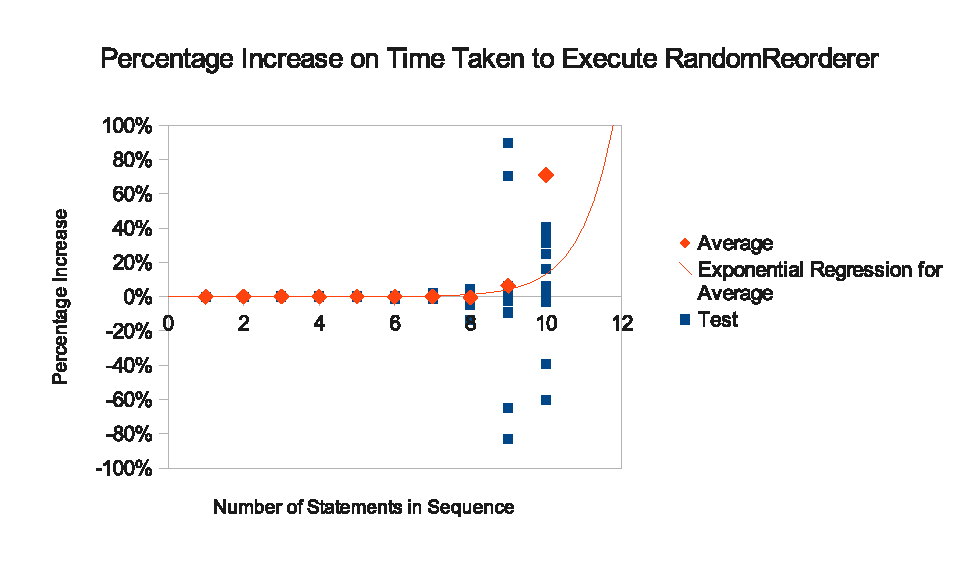
\includegraphics{../images/randomreorderperf.eps}}
\end{figure}

While we can attribute the extra time taken in randomising output to the increasing work undertaken, the sudden increase once statement length
reaches nine could be attributed to Python's garbage collector starting to clean up the extra memory being used. We will now ignore the
\texttt{RandomReorderer} and focus on the effects of a normal reordering using \texttt{Reorderer}.

As we would expect, the average total number of permutations for each sequence length is proportionate to the average time taken to calculate these permutations.
This is shown in the following graph

\begin{figure}[h]
\centering
\scalebox{0.75}
{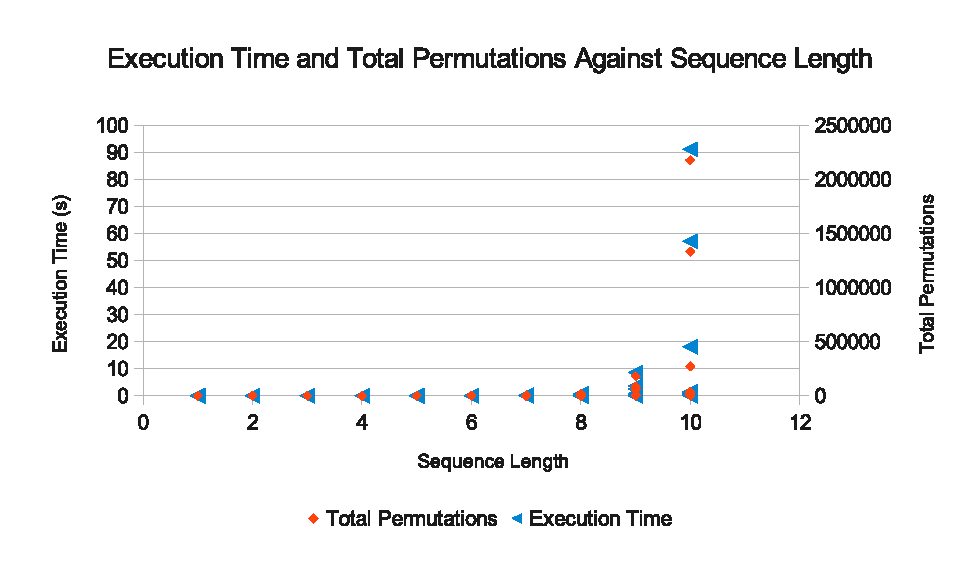
\includegraphics{../images/lengthperf.eps}}
\end{figure}

An unexpected result however is the total number of permutations available on average for each sequence size. If there were no data dependencies, visible statements
or breaking statements we would expect a sequence of length $n$ to yield $n!$ different permutations. As we see in the following graph, the number of permutations
calculable from our generated statement lists are not even close to this limit.

\begin{figure}[h]
\centering
\scalebox{0.75}
{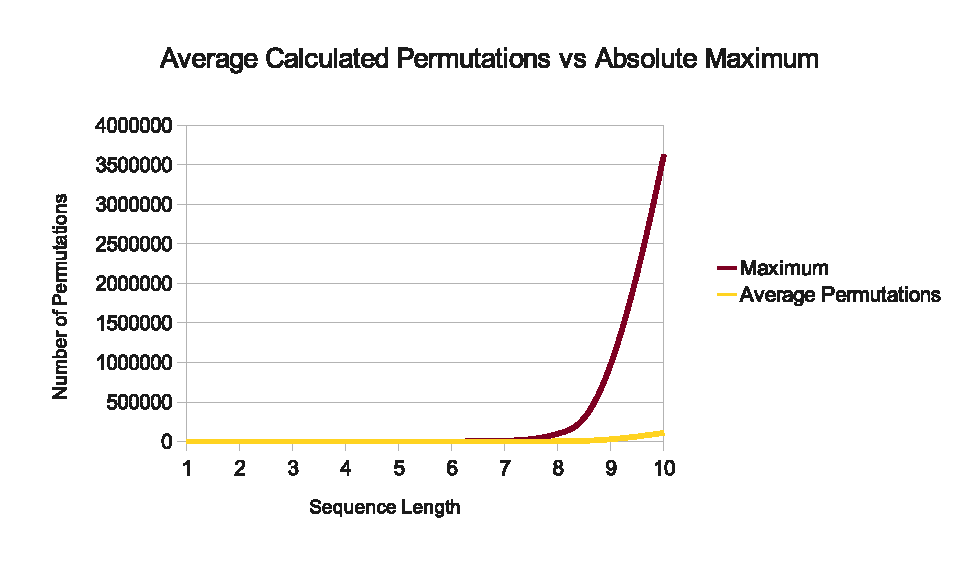
\includegraphics{../images/maxperms.eps}}
\end{figure}

This is likely due to the choice of each of the variables used to generate the statement list. From the following graphs we can see the large
difference that changes in visibility, breaking, read, or write probabilities make.

\begin{figure}[h]
\centering
\subfloat{\scalebox{0.55}{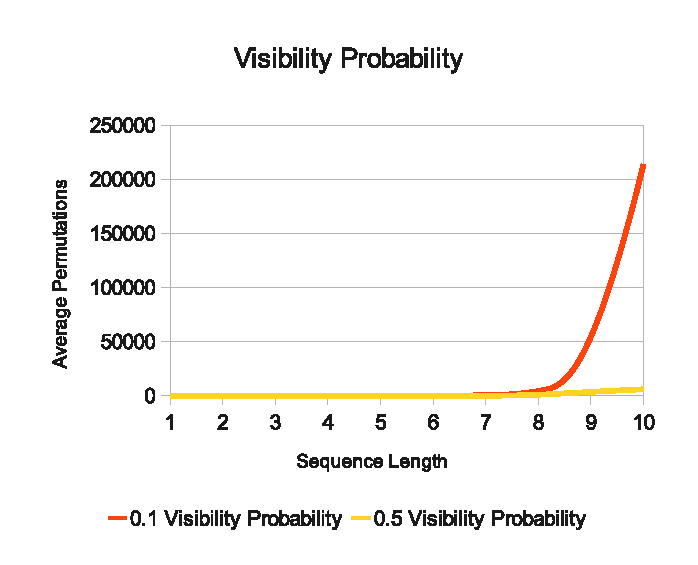
\includegraphics{../images/visprob.eps}}}
\subfloat{\scalebox{0.55}{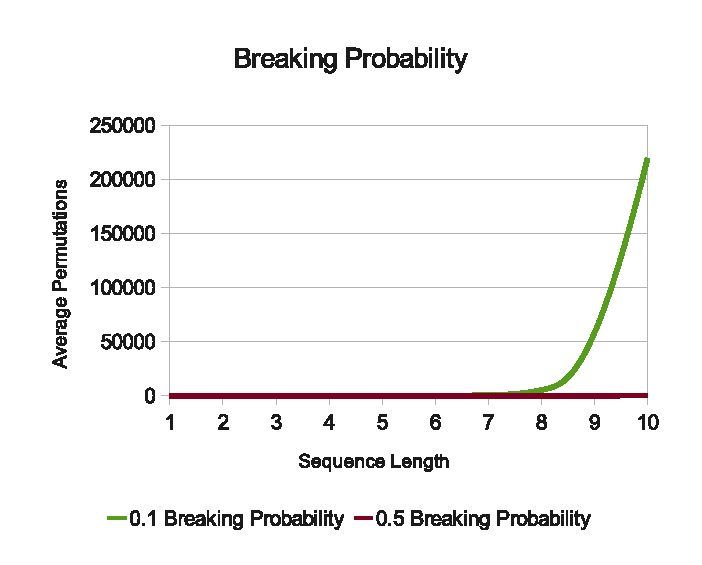
\includegraphics{../images/breakprob.eps}}}
\end{figure}

As we can see, more that a minimal amount of either breaking statements or visible statements severely limits the number of legal permutations we may
generate from a sequence. Of the two types of statements, those that break flow are slightly more effective. This effect means that code with more
visible or breaking statements will be much faster to reorder and have less flexibility in the legal orders available. Similarly the next two graphs show
the effect that differences in the number of reading and writing statements make.

\begin{figure}[h]
\centering
\subfloat{\scalebox{0.55}{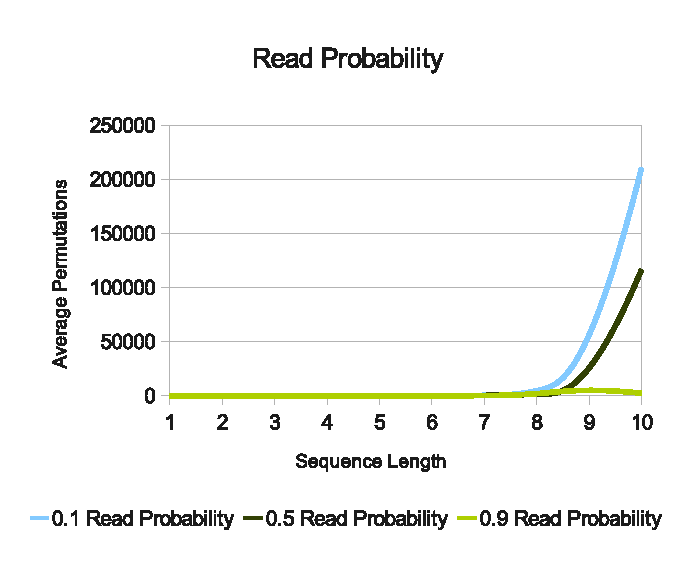
\includegraphics{../images/readprob.eps}}}
\subfloat{\scalebox{0.55}{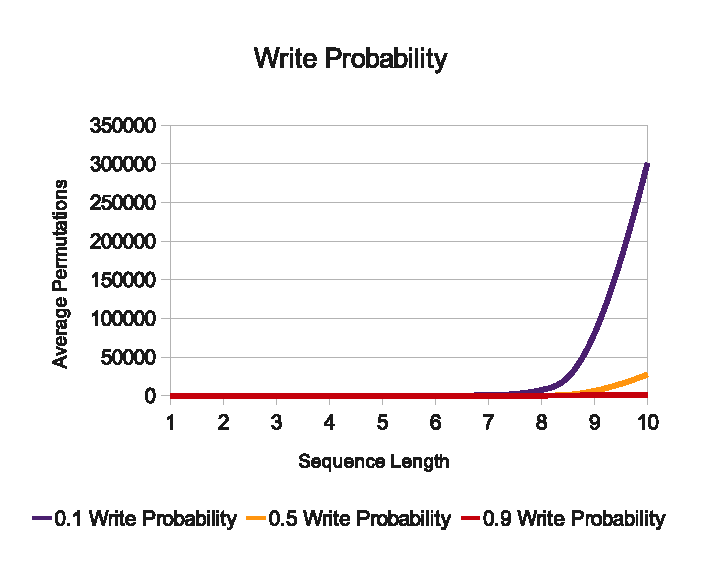
\includegraphics{../images/writeprob.eps}}}
\end{figure}

We see a similar result here to the previous two graphs. The only real difference being that not having many writes inside a sequence of statements
has a greater effect than any of the other variables we have inspected, causing many more legal permutations to become available.

Overall we see that the the maximum number of legal permutations and therefore the maximum expected execution time of a reordering grows exponentially
with the number of statements in the sequence. We tested up to $10$ statements due to the time that testing any more could take, but we can already see
that average number of legal permutations does not grow nearly as fast as it could do. At $10$ statements we see that that execution time maxed at around
$90$ seconds, but averaged only around $3.5$. In a separate test of $10$ independent statements we found that execution time rested at around $120$ seconds,
so most reordering take only a fraction of the maximum time to compute.

By applying this knowledge to our discussion of the strength of our reordering obfuscation we can see that the actual strength depends hugely on the
particular program being obfuscated. If we remember that we can use \texttt{RandomReorderer} and limit its output to the a single permutation we can
create an obfuscation that will stand up to an analyser and possibly a human almost instantaneously. To choose an ideal ordering with the aim of
deobfuscation will depend on attributes we talked about above, and the more legal orderings that an obfuscator can allow, the harder this deobfuscation
will be to perform. Therefore
this obfuscation will be strongest when applied to a program without much visible output or many flow-breaking statements.

\subsection{Irrelevant Branching}

Our aim in inserting new branches into the target source code was to complicate the program and make it less readable or understandable to a human. We will
also confuse an analyser depending on the code inserted.

Other discussions on performing these types of transformations \cite{taxobftrans} tell us that the that the strength and resilience of the obfuscation relies
on the strength of the chosen opaque predicate. As we have not implemented any reverse transformation we cannot quantify the resilience of any particular
predicates. However we can assume that the same problems that have been caused by Python's flexibility during other parts of our implementation will help to thwart
any reversal efforts.

While we do require the user to build up a library of expressions and statements that can be used to insert these irrelevant branches, this allows extra
flexibility. Rather than being limited by what our obfuscator can perform automatically, a user is able to create and insert almost any form of opaque
predicate they like. Although this library may be slow to create initially, once a user has a large base of different examples the process of obfuscating using
them will become much quicker.

To give a very loose idea of how our irrelevant branches will stand up against analysis, we can create a very simple example and allow analysis by
other Python analysers. In fact by testing in all of PyDev \cite{pydev}, pylint \cite{pylint} and PyCharm \cite{pycharm} we see that even the very
simple case below is not recognised as an unreachable branch.

\lstinputlisting{../snippets/deadcode.py}

As such as simple code snippet evades the efforts of dead code analysis from these established tools, we can say with reasonable confidence that even a
simple opaque predicate will stand up to today's Python deobfuscators. Thus a user of our tool must only provide predicates sufficient to outwit a human
analysis.

\section{Conclusions}

We have developed software that allows a user to parse, transform and print any Python 3.x program. From our internal representation we can perform a static
semantic analysis on the program and manually edit or store our findings for future use. Following analysis, our internal representation may be transformed
by either reordering a subset of its statements or by extracting sections of the code into unnecessary and confusing user-defined branches. The transformed
source code may then be written back to file as an obfuscated but still correct version of the original source code.

Our implemented transformations are limited in scope and number. Initially, implementing a reordering operation was intended to be a simple introduction
to the parsing and analysis of Python source code. Instead this seemingly simple problem blossomed into a myriad of separate problems, requiring separate
solutions to implement. Some of these problems were solved by implementing an automatic AST marker for analysis, we use this for calculating which AST nodes
read and write variables or create visible output. Other problems were solved by careful reasoning and restriction of the problem until a `correct' solution
could be reached. This approach was used to restrict the sequences of statements that our reordering transformation could be applied to.

Many of the problems we faced eventually had to be solved by relying on the user's input. One such problem was our inability to resolve function calls to a
particular function definition. Automation of this may be possible to implement for very simple cases and usable during obfuscation, but we could use this
inability to resolve complex function calls to create another form of obfuscation.

The heavy reliance on user input will be a hindrance for using this tool in practice, but there is potential to automate the process and introduce other
tools to help with analysis. If this happens and other forms of obfuscating transformation are implemented then this software could be used successfully
in real situations.

\subsection{Future Work}

There are many possible avenues for extending this work. One of the more pressing issues is to finish the metamorphosis between OAT and GOAT, creating an entire
graphical interface. By doing this we would greatly ease the job of the user, allowing them to simultaneously edit and browse the AST while seeing the changes
made in the source code. The graphical user interface would also be helped by some level of automation, allowing a user to make one or two clicks and have the
entire source file obfuscated by performing different transformations until some level of complexity or time is reached. Once this is done it would be viable
for a user to work with this tool productively.

More technical goals include building a greater number of obfuscating transformations. The architecture or the software allows these to be easily
added to the program so long as they can be implemented at all. Two good candidates for implementation are removal or library calls and idioms and
parallelising code as described the the control-flow obfuscation background section. Removal of library calls would help as a barrier to human reverse
engineering and parallelisation will help greatly against both a machine \textit{and} a human. It would also be helpful to perform some layout obfuscation
by creating a new source writer.

For the ability to implement these new transformations we would also need to perform some more in depth analysis. This would involve developing the ability
to create control flow graphs as well as the ability to transform them back into an ASTs for writing to file. Analysis could then be performed on the CFG,
allowing us hopefully
to resolve function calls or to use constant propagation to break weak opaque predicates. We could use this ability to extend and automate our reordering
operation, removing the user's need to guide the analysis and marking process.

Another useful feature would be to enable the user to work on multiple files at once. This would be much simpler in a graphical interface and would allow
inter-module obfuscation. In allowing this we would enable functions and variables to be split between multiple files, making the job of deobfuscation much
harder. 

Finally it would be helpful to allow the user to automatically test their program following our transformations. This can be used to reassure them that we
have not broken their code. If the user has provided thorough \texttt{doctest}s for their software then these could be automatically performed following any
transformation.

\bibliographystyle{plain}
\bibliography{final}

\end{document}
